\documentclass[a4paper]{book}
\usepackage{notes-style}

%
% 默认情况下itemize的各项间的间距较大,占用文章空间较多,那么如何调整呢?
% https://blog.csdn.net/fandroid/article/details/54644966
% 在导言区进行全局设置,2018-07-05,添加
%
\usepackage{enumitem}
\setenumerate[1]{itemsep=0pt,partopsep=0pt,parsep=\parskip,topsep=5pt}
\setitemize[1]{itemsep=0pt,partopsep=0pt,parsep=\parskip,topsep=5pt}
\setdescription{itemsep=0pt,partopsep=0pt,parsep=\parskip,topsep=5pt}

%
% 每次需要在这里添加图片的路径目录,注意最后面需要有一个 / 2018-07-06 添加
%
\graphicspath{{./figures/chap01/}{./figures/chap02/}{./figures/chap03/}{./figures/chap04/}}  

\def\notesversion{0.01}

\hypersetup{%
  pdftitle={Notes},%
  pdfkeywords={Distributed System, Deep Learning, Neural Networks},
  pdfcreator={XeLaTeX with `ctex' package}
}

% 第四章用到的自定义算符
% \DeclareMathOperator{\argh}{argh}
% \DeclareMathOperator*{\nut}{Nut}
% 第四章的 \proofname 用原先的英文定义
% \def\proofname{Proof}

\makeindex

\begin{document}

\pagenumbering{Alph}

\pdfbookmark{标题页}{title}
\thispagestyle{empty}

\vspace*{\stretch{1}}
\noindent\begin{minipage}{\textwidth}
\raggedleft
{\huge \bfseries 个人学习笔记整理}
\noindent\rule[-1ex]{\textwidth}{5pt}\\[2.5ex]
\hfill\emph{\large 代码阅读笔记、论文阅读报告及一些零散知识点整理}
\end{minipage}

\vspace{\stretch{1}}
\noindent\rlap{%
  \begin{minipage}{\textwidth}
  \linespread{1.67}\selectfont\raggedleft
  {\bfseries 整理:} 刘冰\\
                    qiao.liubing@gmail.com \\[4ex]
  {\bfseries 开始时间:} 7 月 4 日,2018 年\\
  {\bfseries 最后一次更新时间:}~\zhdigits*{\the\year}年\zhnumber{\the\month}月 \\
  {\bfseries 版本:} Version~0.01
  \end{minipage}%
}

\vspace{\stretch{2}}

\newpage\thispagestyle{empty}
\begin{quote}\footnotesize
    Copyright \copyright{}  Bing, Liu. \\
    Permission is granted to copy, distribute and/or modify this document
    under the terms of the GNU Free Documentation License, Version 1.3
    or any later version published by the Free Software Foundation;
    with no Invariant Sections, no Front-Cover Texts, and no Back-Cover Texts.
    A copy of the license is included in the section entitled ``GNU
    Free Documentation License''.
\end{quote}

\frontmatter
% \chapter{中文版致谢}

\section*{5.05 中文版致谢}

对 lshort-zh-cn 的新一轮修订在 China\TeX\ 交流 QQ 群 (91940767) 的网友支持下完成。
参与此次修订的朋友包括:

\begin{center}
\begin{tabular}{lll}
 \toprule
 网友 ID & E-mail \\
 \midrule
 hello   & 312439151@qq.com \\
 $\varepsilon$       & 554502177@qq.com \\
 \bottomrule
\end{tabular}
\end{center}

\noindent\dotfill

\section*{4.20 中文版致谢}

中文 \TeX\ 学会启动的 lshort-zh-cn 修正计划!
本项计划历时八个月,参加的朋友有:

\begin{center}
\begin{tabular}{ll}
\toprule
\textbf{C\TeX 论坛 ID}  & \textbf{翻译章节}  \\
\midrule
zpxing    &   前言、第二章、第五章 1-2.4 {\&} 3、第六章 \\
Frogge    &   第一章  \\
liwenjun  &   第三章  \\
lijian605 &   第四章  \\
gprsnl    &   第五章 2.5-2.11 \\
\bottomrule
\end{tabular}
\end{center}

haginile 和 Frogge 通读了全篇,并给出了详细的勘误表。
blackold 对于第二章亦有所贡献。最后由 zpxing 统筹全书。

\noindent\dotfill

\section*{3.20 中文版致谢}

本文档的翻译工作由 C\TeX{} 版主“经典问题”倡议,历经近十个月才得以完成。
期间参与翻译工作的朋友有:

\begin{center}
\begin{tabular}{lll}
\toprule
\textbf{C\TeX 论坛 ID}  & \textbf{翻译章节}  & \textbf{源文件名} \\
\midrule
经典问题    &   前言    &   overview.tex  \\
高原之狼    &   第一章  &   things.tex   \\
controlong  &   第二章  &   typeset.tex  \\
cxterm      &   第三章  &   math.tex, lssym.tex \\
aloft       &   第四章  &   spec.tex   \\
ganzhi      &   第五章  &   custom.tex \\
\bottomrule
\end{tabular}
\end{center}

\vspace{20pt}

\begin{flushright}
\large\textbf{在此特向这些奉献者表示感谢!}
\end{flushright}

\chapter{英文版致谢}

\noindent Much of the material used in this introduction comes from an
Austrian introduction to \LaTeX\ 2.09 written in German by:
\begin{verse}
\contrib{Hubert Partl}{partl@mail.boku.ac.at}%
{Zentraler Informatikdienst der Universit\"at f\"ur Bodenkultur Wien}
\contrib{Irene Hyna}{Irene.Hyna@bmwf.ac.at}%
   {Bundesministerium f\"ur Wissenschaft und Forschung Wien}
\contrib{Elisabeth Schlegl}{no email}%
   {in Graz}
\end{verse}

If you are interested in the German document, you can find a version
updated for \LaTeXe{} by J\"org Knappen at
\CTAN|info/lshort/german|

\newpage \noindent 
The following individuals helped with corrections, suggestions and
material to improve this paper. They put in a big effort to help me
get this document into its present shape. I would like to
sincerely thank all of them. Naturally, all the mistakes you'll find
in this book are mine. If you ever find a word that is spelled
correctly, it must have been one of the people below dropping me a
line.

\begin{flushleft}\small
Eric~Abrahamsen,        % <eric@ericabrahamsen.net>
Lenimar~Nunes~de~Andrade, % <lenimar@mat.ufpb.br> 12 Nov 1999
Eilinger~August,        % <eaugust@student.ethz.ch>
Rosemary~Bailey,        % <r.a.bailey@qmw.ac.uk> 0.2
Barbara~Beeton,         % <bnb@ams.org>
Marc~Bevand,            % <bevand_m@epita.fr>
Connor~Blakey,          % it's Ligatures!
Salvatore~Bonaccorso,   % <bonaccos@ee.ethz.ch>
Pietro~Braione,         % <braione@elet.polimi.it>
Friedemann~Brauer,      % <fbrauer@is.dal.ca> 3.4
Markus~Br\"uhwiler,     % <m.br@switzerland.org>
Jan~Busa,               % <busaj@ccsun.tuke.sk>
David~Carlisle,         % GONE <carlisle@cs.man.ac.uk> 1.0
Neil~Carter,            % <n.carter@Swansea.ac.uk>
Carl~Cerecke,           % <cdc@cosc.canterbury.ac.nz>
Mike~Chapman,           % <chapman@eeh.ee.ethz.ch> 3.16
Pierre~Chardaire,       % <pc@sys.uea.ac.uk>
Xingyou~Chen,           % <niatlantice@gmail.com> 5.04
Christopher~Chin,       % <chris.chin@rmit.edu.au> 3.1
Diego~Clavadetscher,    % <dc@clavatax.ch>
Wim~van~Dam,            % GONE <wimvdam@cs.kun.nl> 2.2
Benjamin~Deschwanden    % <vdeschwb@student.ethz.ch>
Jan~Dittberner,         % <jan@jan-dittberner.de> 3.15
Michael~John~Downes,    % <mjd@ams.org> 14 Oct 1999
Matthias~Dreier,        % <dreier@ostium.ch>
David~Dureisseix,       % <dureisse@lmt.ens-cachan.fr> 1.1
Hans~Ehrbar,            % <ehrbar@econ.utah.edu>
Elliot,                 % GONE <enh-a@minster.york.ac.uk> 1.1
Rockrush~Engch,         % <niatlantice@gmail.com>
William~Faulk,          % <wfaulk@webassign.net>
Robin~Fairbairns,       % <robin.fairbairns@cl.cam.ac.uk> 0.2 1.0
Johan~Falk,             % <johan@vaxjonexus.com> 5.0.1
J\"org~Fischer,         % <j.fischer@xpoint.at> 3.16
Frank~Fischli,          % <fischlifaenger@gmx.ch>
Daniel~Flipo,           % <daniel.flipo@univ-lille1.fr>
Frank,                  % <frank@freezone.co.uk> 11 Feb 2000
Mic~Milic~Frederickx,   % <mic.milic@web.de>
David~Frey,             % <david@eos.lugs.ch> 2.2
Erik~Frisk,             % <frisk@isy.liu.se> 3.4
Hans~Fugal,             % <hans@fugal.net>
Robert~Funnell,         % <robert.funnell@mcgill.ca> 5.1
Greg~Gamble,            % <gregg@maths.uwa.edu.au> 2.2
Andy~Goth,              % <unununium@openverse.com>
Cyril~Goutte,           % <goutte@ei.dtu.dk> 2.1 2.2
Kasper~B.~Graversen,    % <kbg@dkik.dk>
Arlo~Griffiths,         % <a.griffiths@let.leidenuniv.nl>
Alexandre~Guimond,      % <guimond@iro.umontreal.ca> 0.9
Neil~Hammond,           % <nfh@dmu.ac.uk> 0.3
Christoph~Hamburger,    % <ch.hamburger@gmail.com>
Rasmus~Borup~Hansen,    % GONE <rbhfamos@math.ku.dk> 0.2 0.9 0.91 0.92 1.9.9
Joseph~Hilferty,        % <hilferty@fil.ub.es>
Daniel~Hirsbrunner,     % <dhirsbrunner1@gmail.com>
Martien~Hulsen,         % <m.a.hulsen@Wbmt.tudelft.nl> 1.0 1.1
Bj\"orn Hvittfeldt,     % <bjorn@hvittfeldt.com> 3.13
Morten~H\o gholm,       % <morten.hoegholm@latex-project.org>
Werner~Icking,          % <werner.icking@gmd.de> 3.1
Eric~Jacoboni,          % GONE <jacoboni@enseeiht.fr> 0.1 0.9
Jakob,                  % <diness@get2net.dk>
Alan~Jeffrey,           % <alanje@cogs.sussex.ac.uk> 0.2
Martin~Jenkins,         % xqp.ltd@gmail.com 5.04
Byron~Jones,            % <bj@dmu.ac.uk> 1.1
David~Jones,            % GONE <djones@ca.mcmaster.dcss.insight> 1.1
Johannes-Maria~Kaltenbach, % <kaltenbach@zeiss.de> 3.01
Nils~Kanning,           % <nils@kanning.de>
Andrzej~Kawalec,        % GONE <akawalec@prz.rzeszow.pl> 1.9.9
Christian~Kern,         % <ck@unixen.hrz.uni-oldenburg.de> 2.1
Alain~Kessi,            % <alain_kessi@hotmail.com> 2.2
Axel~Kielhorn,          % <a.kielhorn@web.de>
Sander~de~Kievit,       % <Skievit@ucu.uu.nl>
Kjetil~Kjernsmo,        % <kjetil.kjernsmo@astro.uio.no> 3.2
Tobias~Klauser,		% <tklauser@access.unizh.ch> 4.17
J\"org~Knappen,         % <knappen@vkpmzd.kph.uni-mainz.de> 0.1
Michael~Koundouros,     % <mkoundouros@hotmail.com>
Matt~Kraai,             % <matt.kraai@amo.abbott.com>
Tobias~Krewer,          % <tobias.krewer@googlemail.com>
Flori~Lambrechts,       % <f.lambrechts@softhome.net>
Mike~Lee,               % <rmrstar@gmail.com>
Maik~Lehradt,           % <greek@uni-paderborn.de> 0.1
R\'emi~Letot,           % <r_letot@yahoo.com>
Axel~Liljencrantz,	% <axel.liljencrantz@byv.kth.se>
Jasper~Loy,             % <jasper.loy@gmail.com>
Johan~Lundberg,         % <p99jlu@physto.se>
Martin~Maechler,        % <maechler@stat.math.ethz.ch> 2.2
Alexander~Mai,          % <alexander.mai@physik.tu-darmstadt.de> 3.8
Claus~Malten,           % GONE <asi138%bitnet.djukfa11@bitnet.cearn> 1.1
Kevin~Van~Maren,        % <vanmaren@fast.cs.utah.edu> 24 Nov 1999
Pablo~Markin,
I.~J.~Vera~Mar\'un,     % <i.j.veramarun@ewi.utwente.nl>
Hendrik~Maryns,         % <hendrik.maryns@ugent.be>
Chris~McCormack,        % GONE <chrismc@eecs.umich.edu> 0.1
Aleksandar~S.~Milosevic, % <aleksandar.milosevic@yale.edu>
Henrik~Mitsch,          % <henrik.mitsch@gmx.at>
Stefan~M.~Moser,        % <stefan.moser@ieee.org>
Philipp~Nagele,         % <philipp.nagele@t-systems.com>
Richard~Nagy,           % <r.nagy@nameshield.net>
Manuel~Oetiker,         % <manuel@oetiker.ch>
Urs~Oswald,             % <osurs@bluewin.ch>
Hubert~Partl,           % <partl@mail.boku.ac.at> 0.2 1.1
Marcelo~Pasin,          % <pasin@di.fc.ul.pt>
Martin~Pfister,		% <m@rtinpfister.ch>
Lan~Thuy~Pham,          % <lan.thuy.pham@gmail.com>
Breno~Pietracci,        % <bpietracci@gmail.com>
Demerson~Andre~Polli,   % <polli@linux.ime.usp.br>
Maksym~Polyakov,        % <polyama@myrealbox.com>
Nikos~Pothitos,		% <n.pothitos@di.uoa.gr>
John~Refling,           % <refling@sierra.lbl.gov> 0.1 0.9
Mike~Ressler,           % <ressler@cougar.jpl.nasa.gov> 0.1 0.2 0.9 1.0 1.9.9
Brian~Ripley,           % <ripley@stats.ox.ac.uk> 2.1
Kurt~Rosenfeld,		% <kurt@isis.poly.edu>
Bernd~Rosenlecher,      % <9rosenle@informatik.uni-hamburg.de> 10 Feb 2000
Chris~Rowley,           % <c.a.rowley@open.ac.uk> 0.91
Young~U.~Ryu,           % <ryoung@utdallas.edu> 2.1
Risto~Saarelma,         % <risto.saarelma@cs.helsinki.fi>
Andr{\'a}s~Salamon,     % <andras.salamon@comlab.ox.ac.uk>
Jos\'e~Carlos~Santos,   % <jcsantos@fc.up.pt>
Christopher~Sawtell,    % <csawtell@xtra.co.nz> 1 Sep 1999
Gilles~Schintgen,       % <gschintgen@internet.lu>
Craig~Schlenter,        % <cschle@lucy.ee.und.ac.za> 0.1 0.2 0.9
Hanspeter~Schmid,       % <schmid@isi.ee.ethz.ch>
Baron~Schwartz,         % <bps7j@cs.virginia.edu>
Jordi~Serra~i~Solanich, % <solanich@gmail.com>
Miles~Spielberg,        % <zeibach@hotmail.com>
Susan~Stewart,
Matthieu~Stigler,
Geoffrey~Swindale,      % <geofftswin@ntlworld.com>
Laszlo~Szathmary,       % <szathml@delfin.klte.hu>
Boris~Tobotras,         % <tobotras@jet.msk.su>
Josef~Tkadlec,          % <tkadlec@math.feld.cvut.cz> 2.0 2.2
Scott~Veirs,            % <scottv@ocean.washington.edu>
Didier~Verna,           % <verna@inf.enst.fr> 2.2
Carl-Gustav~Werner,     % <carl-gustav.werner@math.lu.se> 11 Oct 1999, 3.16
Fabian~Wernli,          % <wernli@iap.fr> 3.2
Matthew~Widmann,        % <mtwdmn@gmail.com>
David~Woodhouse,        % <dwmw2@infradead.org> 3.16
Chris~York,             % <c.s.york@Cummins.com> 21 Nov 1999
Rick~Zaccone,           % <zaccone@bucknell.edu> 2.2
Fritz~Zaucker,          % <zaucker@ee.ethz.ch> 3.0
and Mikhail~Zotov.      % <zotov@eas.npi.msu.su> 3.1
\end{flushleft}

\endinput
% \chapter{前言}

\LaTeX\ \cite{manual} 是一个文档准备系统(Document Preparing System),它非常适用于生成高印刷质量
的科技类和数学类文档。它也能够生成所有其他种类的文档,小到简单的信件,大到完整的书籍。
\LaTeX~使用 \TeX\ \cite{texbook} 作为它的排版引擎。%

这份短小的手册描述了 \LaTeXe\ 的使用,对 \LaTeX 的大多数应用来说应该是足够了。
参考文献 \cite{manual,companion} 对 \LaTeX\ 系统提供了完整的描述。%

\bigskip
本手册在英文版 lshort 的基础上进行了适当的重新编排,共有八章和两篇附录:%
\begin{description}%
\item[第一章] 讲述 \LaTeX\ 的来源,源代码的基本结构,以及如何编译源代码生成文档。
\item[第二章] 讲述在 \LaTeX\ 中如何书写文字,包括中文。%
\item[第三章] 讲述文档排版的基本元素——标题、目录、列表、图片、表格等等。结合前一章的内容,你应当能够制作内容较为丰富的文档了。%
\item[第四章] \LaTeX\ 排版公式的能力是众人皆知的。本章的内容涉及了一些排版公式经常用到的命令、环境和符号。
              章节末尾提供了 \LaTeX\ 常见的数学符号。%
\item[第五章] 介绍了如何修改文档的一些基本样式,包括字体、段落、页面尺寸、页眉页脚等。
\item[第六章] 介绍了 \LaTeX\ 的一些扩展功能:排版参考文献、排版索引、排版带有颜色和超链接的电子文档。
\item[第七章] 介绍了如何在 \LaTeX\ 里使用 \TikZ\ 绘图。作为入门手册,这一部分点到为止。
\item[第八章] 当你相当熟悉前面几章的内容,需要自己编写命令和宏包扩展 \LaTeX\ 的功能时,本章介绍了一些基本的命令满足你的需求。
\end{description}%
\begin{description}
\item[附录A] 介绍了如何安装 \TeX\ 发行版和更新宏包。
\item[附录B] 当新手遇到错误和需要寻求更多帮助时,本章提供了一些基本的参考。
\end{description}

\bigskip
这些章节是循序渐进的,建议刚刚熟悉 \LaTeX\ 的读者按顺序阅读。一定要认真阅读例子的源代码,它们贯穿全篇手册,包含了很多的信息。%

\bigskip
如果你已经对 \LaTeX\ 较为熟练,本手册的资源已不足够解决你的问题时,请访问``Comprehensive
\TeX\ Archive Network'' (\texttt{CTAN}) 站点,主页是 \url{www.ctan.org}。
所有的宏包也可以从 \url{mirrors.ctan.org} 和遍布全球的各个镜像站点中获得。

在本书中你会找到其他引用 \texttt{CTAN} 的地方,形式为 \texttt{CTAN://} 和之后的树状结构。
引用本身是一个超链接,点击后将打开内容在 \texttt{CTAN} 上相应位置的页面。

要在自己的电脑上安装 \TeX\ 发行版,请参考附录 \ref{app:install} 中的内容。
各个操作系统下的 \TeX\ 发行版位于 \CTAN|systems|。

\bigskip
如果你有意在这份文档中增加、删除或者改变一些内容,请通知作者。作者对 \LaTeX\ 
初学者的反馈特别感兴趣,尤其是关于这份介绍哪些内容很容易理解,哪些内容可能需要更好地解释,
而哪些内容由于太过难以理解、非常不常用而不适宜放在本手册。

\bigskip
\begin{flushright}
鲁尚文 \\
\mailto|louisstuart96@gmail.com|
\end{flushright}

\vfill

\noindent\begingroup\small lshort 的的最新中文版本位于 \CTAN|info/lshort/chinese|。
如果用户对其他语言的版本感兴趣,请浏览 \CTAN|info/lshort|。\endgroup

\endinput
\tableofcontents
%\listofsources

\mainmatter
\chapter{大规模机器学习框架}\label{chap:large-scale-distributed-deep-learning}
\addtocontents{los}{\protect\addvspace{10pt}}

\begin{intro}
本章内容主要是对知乎上\textit{carbon zhang}的专栏文章\textbf{大规模机器学习框架的四种境界}%
\footnote{https://zhuanlan.zhihu.com/p/29968773}%
进行的总结与整理。
\end{intro}

\section{背景}\label{sec:background}

自从 Google 发表著名的 GFS%
\footnote{The Google File System}、%
MapReduce%
\footnote{MapReduce: Simplified Data Processing on Large Clusters}、%
Big Table% 
\footnote{Bigtable: A Distributed Storage System for Structured Data}%
三篇 paper 以后,互联网正式迎来了大数据时代。

有了 GFS,即分布式文件系统,我们有能力积累海量的数据样本,比如在线广告的曝光和点击数据,天然具有正负样本的特性,
积累一两个月往往就能轻松获得百亿、千亿级的训练样本。这样海量的样本如何存储?用什么样的模型可以学习海量样本中有用
的模式(patterns)?这些问题不止是工程问题,也值得每个做算法的同学去深入思考。

\begin{newnote}[GFS]
Google 在 2003 年发表 GFS 论文,对其中的 Falut Tolerance 有很深刻的印象(第一遍看 GFS 论文的时候)。
\end{newnote}

\begin{newnote}[BigTable]
BigTable 是什么?那篇论文我还没有看过。
\end{newnote}

\subsection{简单模型 or 复杂模型}\label{subsec:simple-or-complex}

在深度学习概念提出之前,我们大都使用的是传统的机器学习算法,例如 LR(逻辑回归)、SVM(支持向量机)、感知机等,这些算法种类很少且相对固定;
那时候要解决一个实际的问题,更多的工作主要集中在\textbf{特征工程}方面。而特征工程本身并没有很系统化的指导理论
(至少目前没有看到系统介绍特征工程的书籍),所以很多时候特征的构造技法显得光怪陆离,是否有用也取决于问题本身、数据样本、模型以及\textbf{运气}。

如果给这种方式起一个名字的话,大概是简单模型+复杂特征;简单模型说的是算法比如 LR、SVM 本身并不复杂,参数和表达能力基本呈现一种线性关系,
易于理解;复杂特征则是指特征工程方面不断尝试使用各种奇技淫巧构造的可能有用、可能没用的特征。这部分特征的构造方式可能会有各种 trick,
比如窗口滑动、离散化、归一化、开方、平方、笛卡尔积、多重笛卡尔积等等;因为特征工程本身并没有特别系统的理论和总结,因此需要大量阅读和自己
业务场景一样或类似的 paper,从里面学习作者分析、理解数据的方法以及对应的构造特征的技法,久而久之,有望形成自己的知识体系。

深度学习概念提出以后,人们发现通过深度神经网络可以进行一定程度的表示学习(representation learning),例如在图像领域,通过 CNN 提取
图像特征(feature) 并在此基础上进行分类,此方法(AlexNet%
\footnote{ImageNet Classification with Deep Convolutional Neural Networks}%
)一举打破了之前算法的天花板,而且是以极大的差距打破。这给所有算法工程师带来了新的思路,既然深度学习本身有提取特征的能力,
干嘛还要苦苦的自己去做人工特征设计呢?

\begin{newnote}[AlexNet]
AlexNet
\end{newnote}

深度学习虽然一定程度上缓解了特征工程的压力,但这里要强调两点:
\begin{enumerate}
\item 缓解并不等于彻底解决。除了图像这种特定领域,在个性化推荐等领域,深度学习目前还没有完全取得绝对的优势;究其原因,可能还是数据自身
内在结构的问题,使得在其他领域目前还没有发现类似图像 + CNN 这样的完美 CP。
\item 深度学习在缓解特征工程的同时,也带来了模型复杂、不可解释的问题。算法工程师在网络结构设计方面一样要花很多心思来提升效果。
\end{enumerate}
概括起来,深度学习代表的简单特征+复杂模型是解决实际问题的另一种方式。

两种模式孰优孰劣还难有定论,以点击率预测为例,在计算广告领域往往以海量特征 + LR 为主流,根据 VC 维理论,LR 的表达能力和特征个数成正比,因此
海量的 feature 也完全可以使 LR 拥有足够的描述能力。而在个性化推荐领域,深度学习刚刚萌芽,目前 google play 采用了 WDL 的结构
\footnote{Wide~\& Deep Learning for Recommender Systems},
YouTube 采用了双重 DNN 的结构\footnote{Deep Neural Networks for YouTube Recommendations}。

\begin{newnote}[VC 维理论]
待补充
\end{newnote}

不管是哪种模式,当模型足够庞大的时候,都会出现模型参数一台机器无法存放的情况。比如百亿级 feature 的 LR 对应的权重 $w$ 有好几十个 G,
这在很多单机上存储都是困难的,大规模神经网络则更复杂,不仅难以单机存储,而且参数和参数之间还有逻辑上的强依赖,要对超大规模的模型进行训练势必
要借用分布式系统的技法,本文主要是系统总结这方面的一些思路。

\begin{newnote}[VGG16 每一层参数所占的空间大小]
待补充 https://zhuanlan.zhihu.com/p/31558973
\end{newnote}

\subsection{数据并行 vs 模型并行}\label{subsec:data-vs-model}

数据并行和模型并行是理解大规模机器学习框架的基础概念,这两个概念在知乎问题『谈谈你对“GPU/CPU 集群下做 Data/Model Parallelism 的区别”的理解?%
\footnote{https://www.zhihu.com/question/31999064}%
』中沐帅给出了一个非常直观且经典的解释:
\begin{quotation}
举个栗子。假设我准备盖一座双子楼,我有两个选择:一个是把人分成两组,每组建一栋楼然后装修好,最后把两个连起来。二是仍然分两组,
第一组先把楼盖好,第二组负责装修。

第一个方案的好处是并行度高。但要求每个组又要懂建房又要懂装修。第二方案要求低点,一个组会建,一个组会装修就行了。坏处是,一个组在干活的时候
另外一个组可能在赋闲。

换成“data/model parallelism”, 这里一个组是一个 cpu 或者一个 gpu。第一个方案是 data parallelism,第二方案是 model parallelism。
技能要求可以简单看成是对内存的需求。当模型很大不能 fit 进单机内存或者单 GPU 内存(这个可能性高多了)的时候,我们一般用 model parallelism,
不然用 data parallelism,因为通常快一些。但某些情况下,model parallelism 的并行程度也没那么低,例如 deep neural network。
换回到那个栗子,每一层楼就是 neural network 的一层。这时候我可以流水盖楼:

第一天:一组盖第一层

第二天:一组盖第二层,二组装修第一层

第三天:一组盖第三层,二组装修第二层$\cdots$

或者只要楼高,可以基本接近2倍加速。
\end{quotation}
第一个方案和数据并行类似,第二个方案则道出了模型并行的精髓。

数据并行理解起来比较简单,当样本比较多的时候,为了使用所有样本来训练模型,不妨把数据分布到不同的机器上,然后每台机器都来对模型参数进行迭代,如图
\ref{fig:data-parallelism} 所示:

\begin{figure}[!hbtp]
\centering
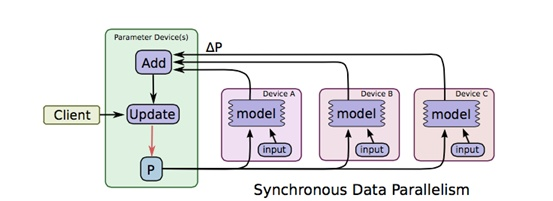
\includegraphics[width=0.85\textwidth]{data-parallelism}
\caption{数据并行}
\label{fig:data-parallelism}
\end{figure}

图片取材于 TensorFlow 的 paper%
\footnote{TensorFlow:Large-Scale Machine Learning on Heterogeneous Distributed Systems},
图中 ABC 代表三台不同的机器,上面存储着不同的样本,模型 P 在各台机器上计算对应的增量 $\Delta$P,然后在参数存储的机器上进行汇总和更新,这就是数据并行。先忽略 synchronous,这是同步机制相关的概念,在第 \ref{subsec:ps-synchronous} 节会有专门介绍。

数据并行概念简单,而且不依赖于具体的模型,因此数据并行机制可以作为框架的一种基础功能,对所有算法都生效。与之不同的是,模型并行因为参数间存在依赖关系
(其实数据并行中参数更新也可能会依赖所有的参数,但区别在于往往是依赖于上一个迭代的全量参数。而模型并行往往是同一个迭代内的参数之间有强依赖关系,比如
DNN 网络的不同层之间的参数依照 BP 算法形成的先后依赖),无法类比数据并行这样直接将模型参数分片而破坏其依赖关系,所以模型并行不仅要对模型分片,
同时需要调度器来控制参数间的依赖关系。而每个模型的依赖关系往往不同,所以模型并行的调度器因模型而异,较难做到完全通用。关于这个问题,CMU 的 Erix Xing 在这里%
\footnote{https://www.jianshu.com/p/00736aa21dc8}
有所介绍,感兴趣的可以参考。

\begin{newnote}[CMU Erix Xing 的分享]
待补充,有文字版整理以及演讲的 PPT
\end{newnote}

\begin{newnote}[现在模型并行的必要性]
ResNet50 模型的整个参数是 100M 左右?现在没有模型并行的需求?全连接层的去除?大家都是在使用着数据并行?

必要性?
\end{newnote}

\begin{newnote}[对于模型并行的调研或相关论文可以推后]
先考察一下现在模型并行的必要性,再开始接触这方面的论文。
\end{newnote}

\noindent\rule[0.25\baselineskip]{\textwidth}{1pt}

模型并行的问题定义可以参考 Jeff Dean 这篇 paper
\footnote{Large Scale Distributed Deep Networks}
,其作为 TensorFlow 的前身,其中图:

\begin{figure}[hbtp]
\centering
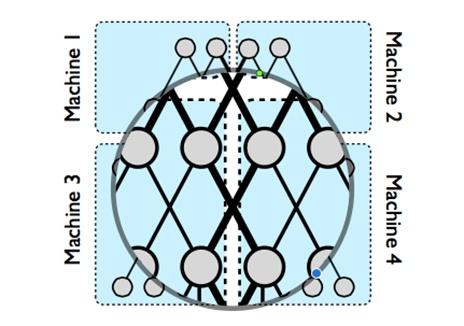
\includegraphics[width=0.6\textwidth]{model-parallelism}
\caption{模型并行}
\label{fig:model-parallelism}
\end{figure}

解释了模型并行的物理图景,当一个超大神经网络无法存储在一台机器上时,我们可以切割网络存到不同的机器上,但是为了保持不同参数分片之间的依赖,
如图中粗黑线的部分,则需要在不同的机器之间进行 concurrent 控制;同一个机器内部的参数依赖,即图中细黑线部分在机器内即可完成控制。

黑线部分如何有效控制呢?如下图所示:

\begin{figure}[hbtp]
\centering
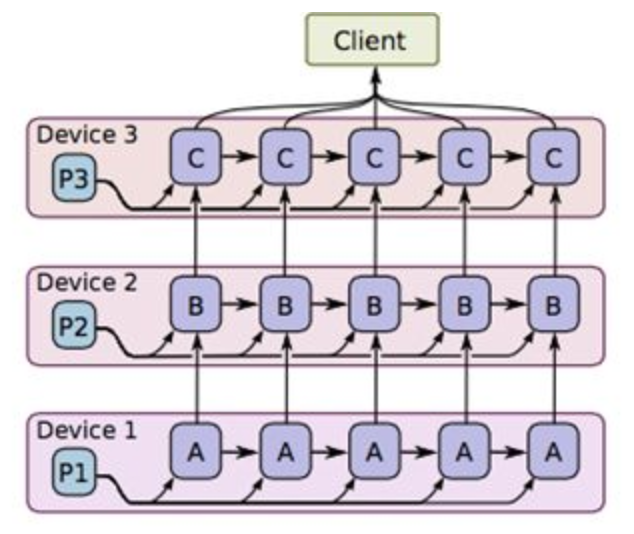
\includegraphics[width=0.6\textwidth]{model-parallelism-training}
\caption{模型并行中的训练过程}
\end{figure}

在将模型切分到不同机器以后,我们将参数和样本一起在不同机器间流转,图中 ABC 代表模型的不同部分的参数;假设 C 依赖 B,B 依赖 A,机器 1 上得到 A 的一个迭代后,
将 A 和必要的样本信息一起传到机器 2,机器 2 根据 A 和样本对 P2 更新得到,以此类推;当机器 2 计算 B 的时候,机器 1 可以展开 A 的第二个迭代的计算。
了解 CPU 流水线操作的同学一定感到熟悉,是的,模型并行是通过数据流水线来实现并行的。想想那个盖楼的第二种方案,就能理解模型并行的精髓了。

\begin{figure}[hbtp]
\centering
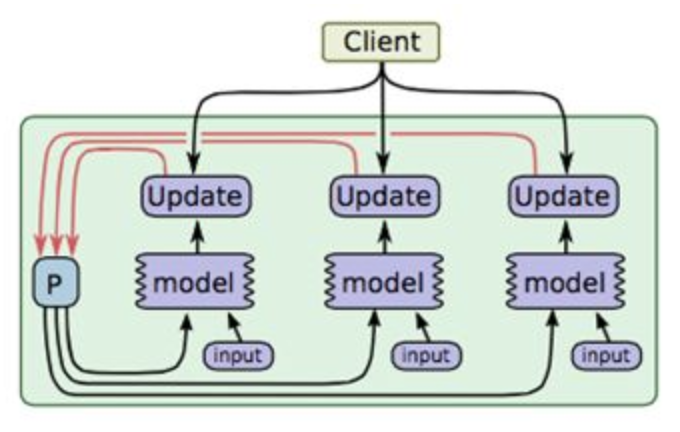
\includegraphics[width=0.65\textwidth]{concurrent-step}
\caption{Concurrent 控制}
\end{figure}

上图则是对控制模型参数依赖的调度器的一个示意图,实际框架中一般都会用 DAG(有向无环图)调度技术来实现类似功能,未深入研究,以后有机会再补充说明。

理解了数据并行和模型并行对后面参数服务器的理解至关重要,但现在让我先荡开一笔,简单介绍下并行计算框架的一些背景信息。

\noindent\textbf{待消化之后补充:}

GPU 上的数据/模型并行与 CPU 集群上的并没有本质区别。从 Fundamental 的角度来说,都是要解决几个问题:
\begin{enumerate}
  \item 通过并行化来做性能加速
  \item 把不可行变为可行(单机内存无法 hold 的 huge model size)
\end{enumerate}

从手段上来说,抽象来看都是这几种:
\begin{enumerate}
  \item 将计算与通信开销overlap以后,提高计算资源的utilization rate[1]
  \item 结合具体的的算法业务场景,对网络的拓扑结构进行优化,在不明显损失精度的情况下,减少并行计算的同步过程所需要传输的数据量
  (典型的例子就是 CNN 里卷积层的 local connectivity,weight sharing,以及 pooling 的设计理念[7])
  \item 将算法与系统相结合,在不明显损失精度的情况下,改善计算资源的utilization rate
  (典型的例子就是Hogwild为代表的ASGD算法[2]以及Eric Xing的团队提出的SSP[3])
\end{enumerate}

具体到操作层面,因为CPU与GPU在计算特点上的差异,还是会引入一些区别: 
\begin{enumerate}
  \item 相较于 CPU 而言,GPU 更强大的『naive』浮点算术能力(这里提到『naive』是为了突出 GPU 硬件设计上忽略复杂的控制结构,
  而把更多的芯片资源用于 computation intensive 的计算逻辑并辅之以 high latency/high bandwidth[8] 的显存资源,来获取到
  浮点计算吞吐能力的显著提升 --- no free lunch 的又一个典型 use case)使得它跟通信的性能 gap 要更为突显,也就使得 GPU 集群上,
  因为计算与通信的 gap 导致的性能 degradation 会更显著。在 GPU 集群里,引入高速通信链路(InfiniBand)以及特定的硬件技术支持
  (GPU Direct  RDMA[11])也都是为了缓解计算与通信的 gap(对于 GPU 与 CPU 计算能力的差异,既不能低估,也不应该过分高估,
  参见 Intel 发在 ISCA10 上的这篇文章[5])。
  \item GPU 的访存特点也使得 GPU 计算平台上能 hold 的有效模型尺寸通常来说是远小于 CPU 平台上的(以比较主流的 Nvidia Tesla K40M[6]为例,
  显存 12GiB),这也使得 GPU 平台上在处理比较大的模型的时候,会比 CPU 平台更早地遇到模型尺寸的瓶颈,需要考虑model parallelism。
  而 GPU 异构计算的复杂性和非黑盒特性也使得 GPU 平台上做 model parallelism 需要考虑更多的 constraint( global memory/shared memory/register file
  这些不同存储单元的延迟及带宽差异),相应会要求更为精巧的设计。
\end{enumerate}

总的来说,我个人以为 GPU 和 CPU 集群上的分布式机器学习系统的搭建并不存在本质上的差异,但是存在操作层面的区别。这些区别的有效
handle 非常依赖于强工程能力,特别是良好的体系结构背景与机器学习 common sense 的有效结合。具体来说,结合硬件的具体指标,
有效平衡好计算与通信的耗时比例,以及 CGMA(Computation to Global Memory Access) ratio[14],对于保证 GPU 集群上的程序性能
是有着重要帮助的。即便是有了 CUDA-Aware MPI[10](OpenMPI 从 1.7.4[12] 开始就已经既支持 InfiniBand 也支持 GPU Direct了),
让编程界面变得跟开发常规 MPI 程序更像了,但是对底层硬件性能指标的精确把握才可能让我们真正用好这些编程 API 完成分布式机器学习系统的开发工作。

再从一个更大的picture来看,分布式机器学习系统,本质上跟常规的分布式系统并没有差异。虽然在Eric Xing的文章[9]里提到了pure-system或pure-algorithm的视角看待分布式学习系统的limitation。但实际上从工业界应用的角度来看mitigate这个limitation所需要的代价其实并不会非常之高(我个人以为Xing教授在Large Scale Learning方面关于异步更新场景下收敛性证明的一些理论性工作对于分布式机器学习系统的未来演进有着方向性的重要意义和价值,但是仅从工业应用的角度来看还并没有构成严格的必要前提条件,有则更佳,欠乏其实并不会影响实际的业务推进和应用)。所以我还是会更愿意把分布式机器学习系统看成分布式系统在特定业务场景下的一个use case。有扎实的分布式系统经验的人,加以专门的Machline Learning相关的培训,其实并不难成长为分布式机器学习系统的专家(五年前,能够用MPI实现并行LR算法,可能还算是相当不错的技术成绩。而现在,一个基础扎实的应届生,给他合适的mentorship,其实花两三个月的时间也就能够实现一个可用于支持线上生产训练任务的版本了)。

现在,因为技能本身的diversity,拥有分布式机器学习系统开发经验的工程师还是稀缺资源,但是我会有这样一种感觉,随着时间的推移,人才的流动,会有更多的人能够掌握相关的经验技能,这个技能的稀缺性也会渐渐地下降到一个稳定值。大规模机器学习系统的Cross-domain性质所带来的固有难度还是存在一个固有的门坎,但是在我看来,这些门坎更多是一些know-how性质的门坎,而不是fundamental的门坎,是可以通过建立有效的培养机制来解决掉的。举例来说,不理解L1和L2正则为什么一个对应于Laplace先验,另一个对应于高斯先验,并不会影响我们去实现相应的分布式L1/L2 LR算法;同样,对矩阵分解理论缺乏精细的理解和把控,也不会构成我们去实现一个SVDFeature或是Tensor Decomposition算法的本质障碍;没有办法把EM算法的原理推敲得很清楚,也不会影响我们去实现一个并行版的PLSA主题模型。从工程实现的角度去完成一个academia community设计出来的大规模机器学习算法和自已从头设计一个大规模机器学习算法所需要的背景知识还是不一样的。前者更适合工业界的同学来完成,后者则更适合academia的同学来担当。(注意,我上面说的都是大规模算法的实现,而不是大规模算法的应用,我个人的观点,真正要把这些算法有效地应用到业务场景里,难度反而更大,不是仅仅靠良好的engineering practice和machline learning common sense就可以做到的,而会需要更扎实的数理统计以及数据挖掘/机器学习的专业背景)

个人来说,我更期待学术界能够从更fundamental的层面为large scale learning提供支持。因为现在的large scale learning系统在工业界的应用,我觉得还更多是一种以embarrassingly parallel为代表的暴力式方法带来性能优化。data parallelism/model parallelism不外如是,ASGD也算是一个“暴力”性质的例子(异步SGD虽然看起来很美,但是从实际的implementation上来看,在不同数据集上保证良好的收敛性并不是件容易的事情,在带来计算资源的更有效utilization rate的同时,ASGD固有的随机性其实让达到相同收敛点所需耗费的时间更长,变数也更多。G家的Paper[4]虽然claim说在non-convex, non-sparse场景下,他们使用ASGD+Adagrad也能够获得不错的收敛效果,但是缺失了严格的理论证明总会让人猜测有一些论文中没有透露的tricks才使得他们保证了ASGD在不同数据集上的收敛能力)。这种”暴力美学“性质的优化工业界有足够的能力去handle,而工业界因其自身定位特别是业务压力,未必有能力和精力handle的则是一些通过算法设计改良将算法时间复杂度或空间复杂度大幅降下来的case,典型的例子就是Newton法之于Gradient Descent,LBFGS算法之于原生的BFGS算法。以及对算法改良的theory justification,比如Eric Xing的团队在bounded delay场景下异步更新收敛性证明方面做过的一些工作。

最后简单summarize一下:
\begin{enumerate}
  \item GPU与CPU集群上Model/Data Parallelism不存在本质上的区别,更多是存在工程细节上的区别。对这些工程细节的有效handle依赖于强体系结构背景和机器学习 common sense的有机结合。
  \item 大规模机器学习系统本质上可以视为分布式系统的一个特例。虽然现在从事大规模机器学习系统开发还算是稀缺能力,但是开发大规模机器学习系统所需的技能经验是可以通过有效的培养机制加以养成的。
  \item 为了担心误导,特地加入对2的补充。只是开发出可以用于支持线上常规业务(CTR Prediction/搜索推荐/文本潜层语义挖掘,以及比较成熟的Deep Learning应用场景—Speech and CV)的大规模机器学习系统的技能经验是不难培养的,但是真正顶尖的相关能力则是不太容易培养的(似乎任何行当都是如此)。在资讯发达,行业交流频繁的年代,只是写一个可以work并支持线上业务基本需求的大规模并行算法并不存在本质困难(就算是一些现在不知道应该怎么做的算法,随着时间推移也不难从别人那里听说个大概,自然也就可以完成相应的实现了),但是结合业务场景,进行算法定制,来帮助业务建立起技术壁垒,就需要在engineering practice, machline learning common sense之外,对domain knowledge(既指代技术知识,也包括业务知识)建立起更深刻的理解和把握了,这种能力是需要通过长时间的思考,沉淀,持续地追踪最新的学术进展,同时touch多个domain才可能建立起来的,非量产品。
\end{enumerate}

\begin{itemize}
  \item [Alex2014] One Weird Trick for Parallelizing CNN
  \item [Niu2011] Hogwild!: A lock-free approach to parallelizing stochastic gradient descent 
  \item [Qirong2013] More Effective Distributed ML via a Stale Synchronous Parallel Parameter Server
  \item [Jeff2012]Large scale distributed deep networks 
  \item [Victor2010]Debunking the 100X GPU vs. CPU Myth: An Evaluation of Throughput Computing on CPU and GPU
  \item [Nvidia官网]http://www.nvidia.com/content/PDF/kepler/nvidia-tesla-k40.pdf
  \item [Jarret2009]What is the Best Multi-Stage Architecture for Object Recognition? 
  \item [Patterson]Why Latency Lags Bandwidth, and What it Means to Computing 
  \item [Eric2014]http://www.cs.cmu.edu/~epxing/talks/IEEE2014-BigData-Tutorial.pdf
  \item [Nvidia官网]NVIDIA GPUDirect https://developer.nvidia.com/gpudirect
  \item [Nvidia官网]http://on-demand.gputechconf.com/gtc/2013/presentations/S3047-Intro-CUDA-Aware-MPI-NVIDIA-GPUDirect.pdf
  \item [OpenMPI GitHub]https://github.com/open-mpi/ompi/
  \item [David B.Kirk2013]Programming Massively Parallel Processors, 2nd Edition, Chapter 5, Section 5.1
\end{itemize}

整理自:https://www.zhihu.com/question/31999064/answer/54185461

\begin{newnote}[模型并行带来的两方面益处]
对神经网络进行划分,比如水平、垂直划分等等,模型并行带来了两方面的益处
\begin{itemize}
  \item 能处理更大规模的模型,因为单机内存有限,特别是 GPU 内存
  \item 带来了流水线优化,提升了计算效率。
\end{itemize}
但也有缺点,比如在水平划分模型时,中间的某一层计算需要上一层所有的数据都计算完毕,如果有数据未完成,整个计算都会延迟,也就是木桶效应
(计算效率由最慢的计算决定,而水平模型划分加剧了这类风险)。这里就可以用体系结构的方法来处理这些问题了。

但数据并行和模型并行,二者本质上没有区别,都是为了提高并行度,增加计算效率,最大化利用计算资源。但是模型并行还能够带来对更大规模的
神经网络的处理能力。

整理自:https://www.zhihu.com/question/31999064/answer/106715799
\end{newnote}

\begin{newnote}[GPU 内存]

\end{newnote}

\noindent\rule[0.25\baselineskip]{\textwidth}{1pt} %% TODO


\section{并行算法演进}\label{sec:para-algorithms}

\subsection{MapReduce 路线}\label{subsec:mapreduce}

从函数式编程中的受到启发,Google 发布了 MapReduce 的分布式计算框架,通过将任务切分成多个叠加的 Map+Reduce 任务,来完成复杂的计算任务,示意图如下

\begin{figure}[!hbtp]
\centering
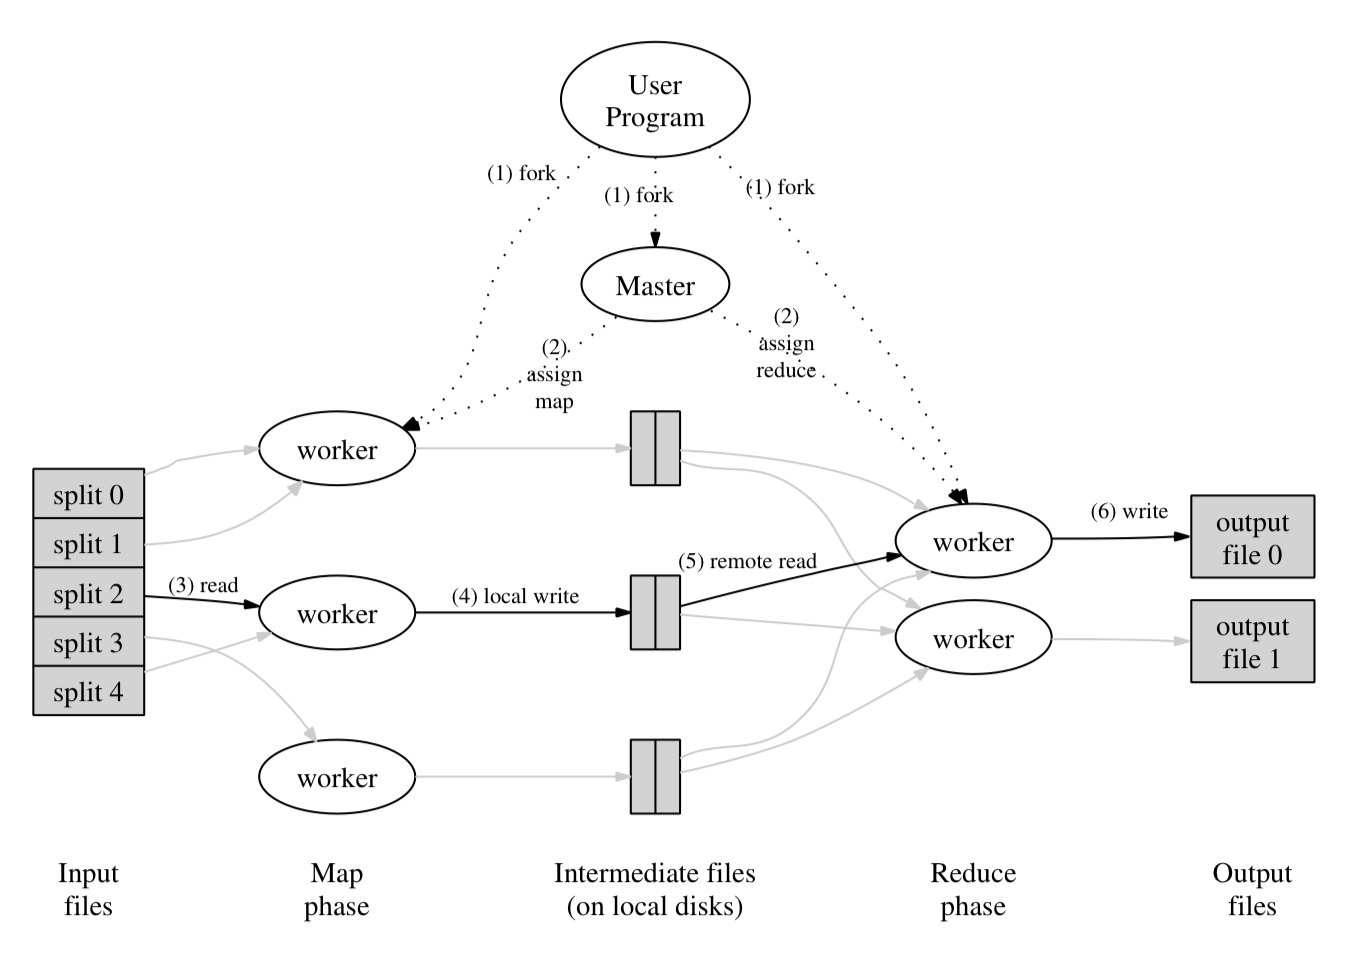
\includegraphics[width=0.85\textwidth]{map-reduce}
\caption{MapReduce 的整个流程}
\end{figure}

\begin{newnote}[MapReduce]
MapReduce 是一种编程模型。\textbf{阅读 MapReduce 论文,写阅读笔记。}  %% TODO
\end{newnote}

MapReduce 的主要问题有两个:
\begin{enumerate}
  \item 原语的语义过于低级,直接使用其来写复杂算法,开发量比较大;
  \item 依赖于磁盘进行数据传递,性能跟不上业务需求。
\end{enumerate}

为了解决 MapReduce 的两个问题,Matei 提出了一种新的数据结构 RDD%
\footnote{},
并构建了 Spark 框架。Spark 框架在 MapReduce 语义之上封装了 DAG 调度器,极大降低了算法使用的门槛。

\begin{newnote}[RDD]
RDD 弹性数据集。\textbf{阅读 Spark 论文,写阅读笔记。}  %% TODO
\end{newnote}

较长时间内 Spark 几乎可以说是大规模机器学习的代表,直至后来沐帅的参数服务器进一步开拓了大规模机器学习的领域以后,Spark 才暴露出一点点不足。如下图:

\begin{figure}[hbtp]
\centering
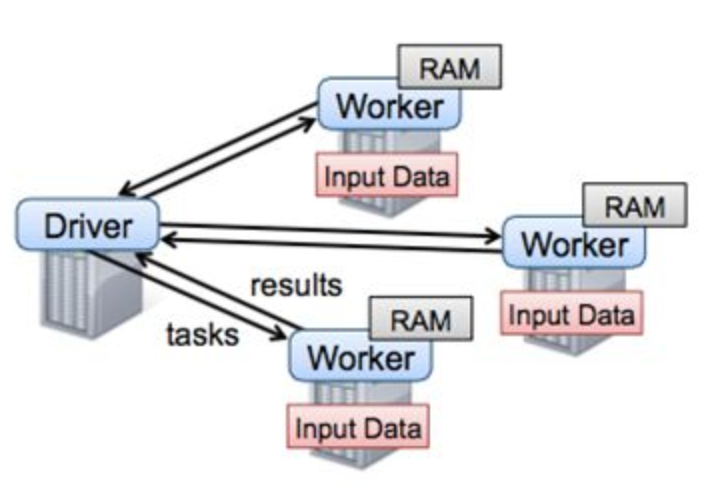
\includegraphics[width=0.65\textwidth]{spark-architecture}
\caption{Spark 的架构}
\end{figure}

从图中可以看出,Spark 框架以 Driver 为核心,任务调度和参数汇总都在 Driver,而 Driver 是单机结构,所以 Spark 的瓶颈非常明显,就在 Driver 这里。
当模型规模大到一台机器存不下的时候,Spark 就无法正常运行了。所以从今天的眼光来看,Spark 只能称为一个中等规模的机器学习框架。腾讯开源的 Angel 通过修改 Driver 的底层协议将 Spark 扩展到了一个高一层的境界。后面还会再详细介绍这部分。

\begin{newnote}[Spark]
Spark 是一个内存计算框架。
\end{newnote}

MapReduce 不仅是一个框架,还是一种思想,Google 开创性的工作为我们找到了大数据分析的一个可行方向,时至今日,仍不过时。
只是逐渐从业务层下沉到底层语义应该处于的框架下层。


\subsection{MPI技术}\label{subsec:mpi}

沐帅在知乎问题『MPI 在大规模机器学习领域的前景如何?%
\footnote{https://www.zhihu.com/question/55119470}』%
中对MPI的前景做了简要介绍:
\begin{quotation}
这个取决于场景,如果要在超算(super computer)上跑机器学习,用 MPI 是不错的选择。但在云上,不管是公有云的例如 AWS/Azure/GCP 或者私有云,MPI
没有太多必要。

MPI 定义的是接口,具体用的时候我们是用某个特定的实现,例如 openmpi 或者 mpich2。 为了简单,这里统一叫 MPI。

用  MPI 实现机器学习是没问题的,不管是对高维稀疏模型还是深度学习。MPI 的接口在一些算法的实现上很方便,另外一些地方(例如异步)绕一绕也是可以的。
例如虽然 MXNet 没有用 MPI,不过使用 MPI 来实现个 kvstore 的 backend 也是可行的。

MPI 的一大优势是支持各种网络硬件,例如 infiniband 和 Intel Omni Path,或者网络拓扑结构,例如 cray 的 dragonfly。通常 MPI 会做各种针对性的优化从而得到不错的性能。

这个优势主要体现在超算上。而对于云,通常使用常见的网络硬件(例如Ethernet)和连接结构(multi-rooted tree),MPI 做的优化通常不会有太大效果。
在云上,MPI 的一大问题是容灾。任何一个节点出问题会导致整个任务失败,会导致运营成本增加。(回答里面有提到百度有 MPI 集群。我当年是最大的用户,
一度使用超过50\% 的节点。对于这一点我是深有体会,例如凌晨 3 点起来重启任务。)

所以结论是,如果要在云上跑机器学习的话,MPI 前景不大。但如果是使用 Top500 类似的超算,MPI 是不错的选择。
\end{quotation}

和 Spark 不同,MPI 是类似 socket 的一种系统通信 API,只是支持了消息广播等功能。因为对 MPI 研究不深入,这里简单介绍下优点和缺点吧。
优点是系统级支持,性能杠杠的;缺点也比较多,一是和 MapReduce 一样因为原语过于低级,用 MPI 写算法,往往代码量比较大。另一方面是基于 MPI 的集群,
如果某个任务失败,往往需要重启整个集群,而 MPI 集群的任务成功率并不高。阿里的鲲鹏系统%
\footnote{KunPeng:Parameter Server based Distributed Learning Systems and Its Applications in
Alibaba and Ant Financial}%
给出了下图:

\begin{figure}[hbtp]
\centering
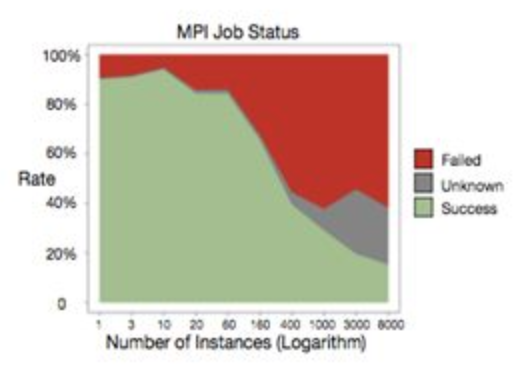
\includegraphics[width=0.85\textwidth]{mpi-task-success-rate}
\caption{MPI 集群的任务成功率}
\end{figure}

从图中可以看出,MPI 作业失败的几率接近五成。MPI 也并不是完全没有可取之处,正如沐帅所说,在超算集群上还是有场景的。对于工业届依赖于云计算、依赖于
commodity 计算机来说,则显得性价比不够高。当然如果在参数服务器的框架下,对单组 worker 再使用 MPI 未尝不是个好的尝试,鲲鹏系统正是这么设计的。

\begin{newnote}[MPI]
因为对 MPI 在之前基本就没有怎么了解过,考察一下,如果 MPI 现在使用的还比较广泛,这个可能需要整理成一个新的章节来。 %% TODO
\end{newnote}


\section{参数服务器演进}\label{subsec:ps-revolution}

\subsection{历史演进}\label{subsec:ps-history}

沐帅在 OSDI2014 的一篇文章%
\footnote{Scaling Distributed Machine Learning with the Parameter Server}% TODO 
中将参数服务器的历史划分为三个阶段,第一代参数服务器萌芽于沐帅的导师 Smola 的 paper%
\footnote{An Architecture for Parallel Topic Models}%
,如下图所示:

\begin{figure}[hbtp]
\centering
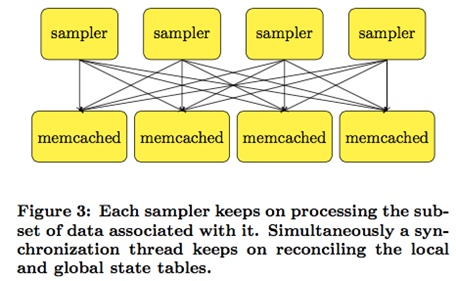
\includegraphics[width=0.85\textwidth]{topic-model}
\caption{xxxxxx待补充}
\end{figure}

这个工作中仅仅引入 memcached 来存放 key-value 数据,不同的处理进程并行对其进行处理。另一篇文章%
\footnote{Piccolo:Building fast, distributed programs with partitioned tables}%
中也有类似的想法。第二代参数服务器叫 application-specific 参数服务器,主要针对特定应用而开发,其中最典型的代表应该是 TensorFlow 的前身 DistBelief%
\footnote{Large Scale Distributed Deep Networks}。

第三代参数服务器,也即是通用参数服务器框架是由百度少帅李沐正式提出的,和前两代不同,第三代参数服务器从设计上就是作为一个通用大规模机器学习框架来定位的。
要摆脱具体应用、算法的束缚,做一个通用的大规模机器学习框架,首先就要定义好框架的功能;而所谓框架,往往就是把大量重复的、琐碎的、做了一次就不想再来第二次的脏活、累活
进行良好而优雅的封装,让使用框架的人可以只关注于自己的核心逻辑。第三代参数服务器要对哪些功能进行封装呢?沐帅总结了这几点,我照搬如下:

\begin{itemize}
  \item \textbf{高效的网络通信:}异步通信,计算与通信重叠(overlap);
  \item \textbf{灵活的一致性模型:}不同的一致性模型其实是在模型收敛速度和集群计算量之间做 tradeoff,要理解这个概念需要对模型性能的评价做些分析,
  暂且留到下节再介绍;
  \item \textbf{弹性可扩展:}新节点的加入不需要重启整个运行的框架;
  \item \textbf{容灾容错:}大规模集群协作进行计算任务的时候,出现Straggler或者机器故障是非常常见的事,因此系统设计本身就要考虑到应对;没有故障的时候,
  也可能因为对任务时效性要求的变化而随时更改集群的机器配置。这也需要框架能在不影响任务的情况下能做到机器的热插拔;
  \item \textbf{易用性:}主要针对使用框架进行算法调优的工程师而言,显然,一个难用的框架是没有生命力的。
\end{itemize}

在正式介绍第三代参数服务器的主要技术之前,先从另一个角度来看下大规模机器学习框架的演进。
 
\begin{figure}[hbtp]
\centering
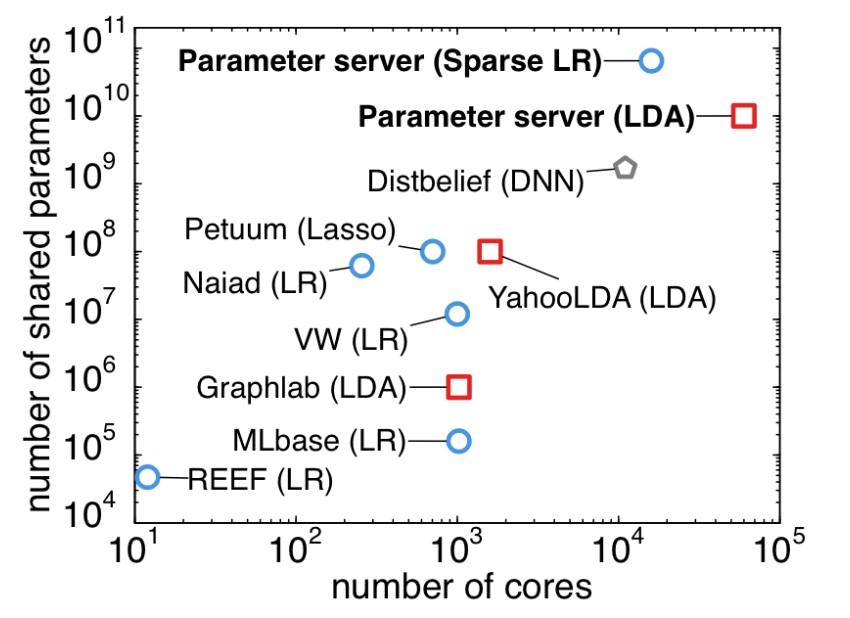
\includegraphics[width=0.65\textwidth]{ps-compare-with-others}
\caption{参数服务器与其他系统执行执行机器学习任务的比较}
\label{fig:ps-compare-with-others}
\end{figure}

这张图可以看出,在参数服务器出来之前,人们已经做了多方面的并行尝试,不过往往只是针对某个特定算法或特定领域,比如 YahooLDA 是针对 LDA 算法的。
当模型参数突破十亿以后,则可以看出参数服务器一统江湖,再无敌手。

\subsection{基础架构}\label{subsec:ps-architecture}

第三代参数服务器的基本架构

\begin{figure}[hbtp]
\centering
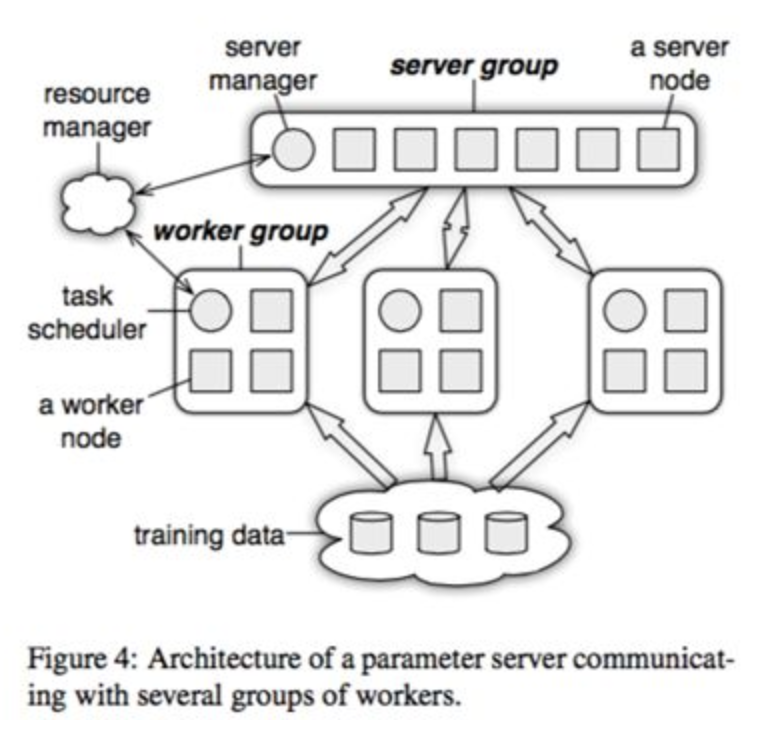
\includegraphics[width=0.85\textwidth]{ps-architecture}
\caption{xxxxxx待补充}
\end{figure}

上图的 resource manager 可以先放一放,因为实际系统中这部分往往是复用现有的资源管理系统,比如 yarn 或者 mesos;
底下的 training data 毋庸置疑的需要类似 GFS 的分布式文件系统的支持;剩下的部分就是参数服务器的核心组件了。

图中画了一个 server group 和三个 worker group;实际应用中往往也是类似,server group 用一个,而 worker group 按需配置;
server manager 是 server group 中的管理节点,一般不会有什么逻辑,只有当有 server node 加入或退出的时候,为了维持一致性哈希而做一些调整。

worker group 中的 task schedule 则是一个简单的任务协调器,一个具体任务运行的时候,task schedule 负责通知每个 worker 加载自己对应的数据,
然后去 server node 上拉取一个要更新的参数分片,用本地数据样本计算参数分片对应的变化量,然后同步给 server node;server node在收到本机负责的
参数分片对应的所有 worker 的更新后,对参数分片做一次 update。

\begin{figure}[hbtp]
\centering
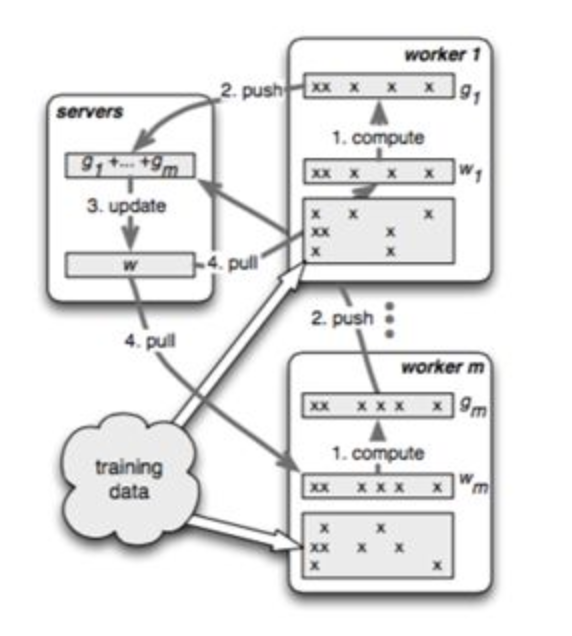
\includegraphics[width=0.65\textwidth]{ps-sub-sgd}
\caption{xxxxxx待补充}
\end{figure}

如图所示,不同的 worker 同时并行运算的时候,可能因为网络、机器配置等外界原因,导致不同的 worker 的进度是不一样的,如何控制 worker 的同步机制
是一个比较重要的课题。详见下节分解。

\textbf{ps-lite 代码详细解析}  %% TODO

\subsection{同步协议}\label{subsec:ps-synchronous}

本节假设读者已经对随机梯度优化算法比较熟悉,如果不熟悉的同学请参考吴恩达经典课程机器学习中对 SGD 的介绍,或者我之前多次推荐过的书籍
《{\color{red}最优化导论}》。

我们先看一个单机算法的运行过程,假设一个模型的参数切分成三个分片 k1,k2,k3;比如你可以假设是一个逻辑回归算法的权重向量被分成三段。我们将训练样本
集合也切分成三个分片 s1,s2,s3;在单机运行的情况下,我们假设运行的序列是(k1,s1)、(k2,s1)、(k3、s1)、(k1、s2)、(k2、s2)、(k3、s2)
$\dots$ 看明白了吗?就是假设先用 s1 中的样本一次对参数分片 k1、k2、k3 进行训练,然后换 s2;这就是典型的单机运行的情况,而我们知道这样的运行序列
最后算法会收敛。

现在我们开始并行化,假设 k1、k2、k3 分布在三个 server node 上,s1、s2、s3 分布在三个 worker node 上,这时候如果我们还要保持之前的计算顺序,
则会变成怎样?work1 计算的时候,work2 和 worker3 只能等待,同样 worker2 计算的时候,worker1 和 work3 都得等待,以此类推;可以看出这样的
并行化并没有提升性能;但是也算简单解决了超大规模模型的存储问题。

为了解决性能的问题,业界开始探索这里的一致性模型,最先出来的版本是前面提到的的ASP模式%
\footnote{An Architecture for Parallel Topic Models}% TODO 这篇文章在 TensorFlow 2016 年的文章中开始部分有提及到
,就是完全不顾 worker 之间的顺序,每个 worker 按照自己的节奏走,跑完一个迭代就 update,然后继续,这应该是大规模机器学习中的 freestyle 了,如图所示

\begin{figure}[hbtp]
\centering
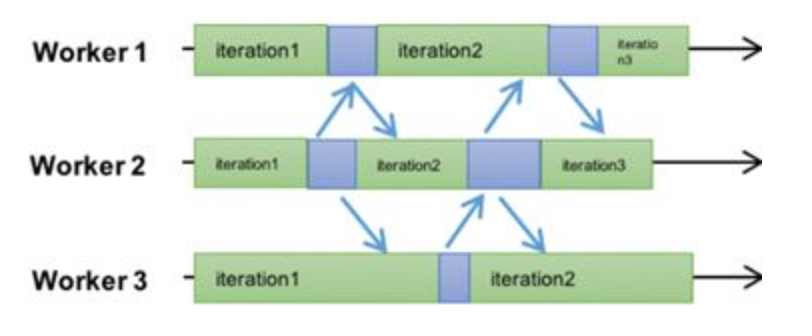
\includegraphics[width=0.85\textwidth]{asp}
\caption{ASP 模式}
\end{figure}

ASP 的优势是最大限度利用了集群的计算能力,所有的 worker 所在的机器都不用等待,但缺点也显而易见,除了少数几个模型,比如 LDA,ASP 协议可能导致模型无法收敛。
也就是 SGD 彻底跑飞了,梯度不知道飞到哪里去了。

在 ASP 之后提出了另一种相对极端的同步协议 BSP,Spark 用的就是这种方式,如图所示

\begin{figure}[hbtp]
\centering
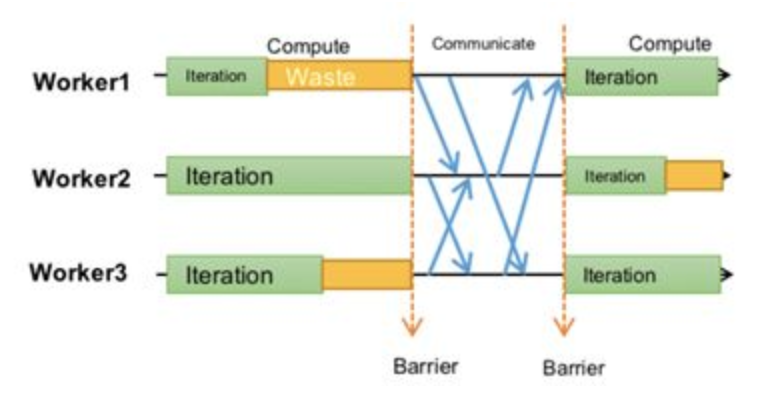
\includegraphics[width=0.85\textwidth]{bsp}
\caption{BSP 模式}
\end{figure}

每个 worker 都必须在同一个迭代运行,只有一个迭代任务所有的 worker 都完成了,才会进行一次 worker 和 server 之间的同步和分片更新。
这个算法和严格一致的算法非常类似,区别仅仅在于单机版本的 batch size 在 BSP 的时候变成了有所有 worker 的单个 batch size 求和
得到的总的 batch size 替换。毫无疑问,BSP 的模式和单机串行因为仅仅是 batch size 的区别,所以在模型收敛性上是完全一样的。同时,
因为每个 worker 在一个周期内是可以并行计算的,所以有了一定的并行能力。

以此协议为基础的 Spark 在很长时间内成为机器学习领域实际的霸主,不是没有理由的。此种协议的缺陷之处在于,整个 worker group 的性能由其中最慢的 worker 决定;这个 worker 一般称为 straggler。读过 GFS%
\footnote{The Google File System}%
文章的同学应该都知道 straggler 的存在是非常普遍的现象。

\begin{newnote}[GFS 中的 Straggler]
阅读 GFS 中的 Straggler 部分  %% TODO
\end{newnote}

能否将 ASP 和 BSP 做一下折中呢?答案当然是可以的,这就是目前我认为最好的同步协议 SSP;SSP 的思路其实很简单,既然 ASP 是允许不同 worker 之间的
迭代次数间隔任意大,而 BSP 则只允许为 0,那我是否可以取一个常数 s?如图所示

\begin{figure}[hbtp]
\centering
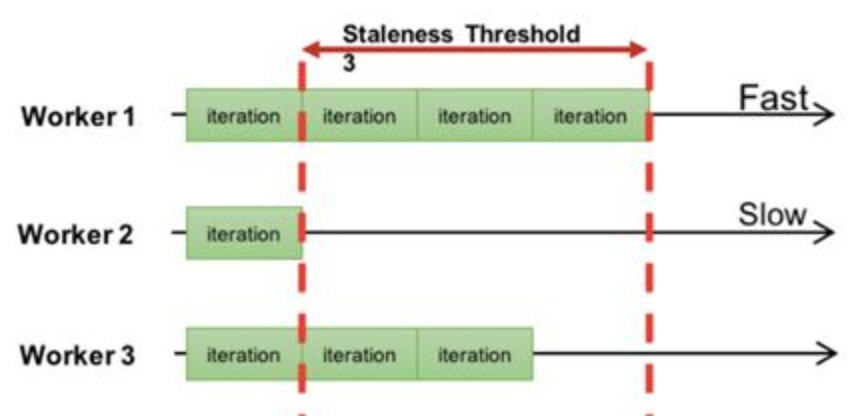
\includegraphics[width=0.85\textwidth]{ssp}
\caption{SSP 模式}
\end{figure}

不同的 worker 之间允许有迭代的间隔,但这个间隔数不允许超出一个指定的数值 s,图中 s=3.

SSP 协议的详细介绍参见%
\footnote{More Effective Distributed ML via a Stale Synchronous Parallel Parameter Server}%  TODO 这篇文章真是很有开创性啊!
,CMU 的大拿 Eric Xing 在其中详细介绍了 SSP 的定义,以及其收敛性的保证。理论推导证明常数 s 不等于无穷大的情况下,算法一定可以在若干次迭代以后进入收敛状态。
其实在 Eric 提出理论证明之前,工业界已经这么尝试过了:)

\begin{newnote}[从另一个角度看数据并行]
在随机梯度下降中,数据并行使用参数服务器(Parameter Server)来做同步,同步的策略就是我们上面提到的 ASP、BSP 以及 SSP。在 GeePS
中,提到同步策略对更新效率的影响,BSP 最好,SSP 次优,ASP 最差;但 BSP 每轮都需要同步,训练一批数据时间会最长,SSP 次优,ASP 最快。
所以这就是一个 tradeoff 的问题了:如何选择同步策略?

GeePS: Scalable deep learning on distributed GPUs with a GPU-specialized parameter server  %% TODO

整理自:https://www.zhihu.com/question/31999064/answer/106715799
\end{newnote}

\begin{figure}[hbtp]
\centering
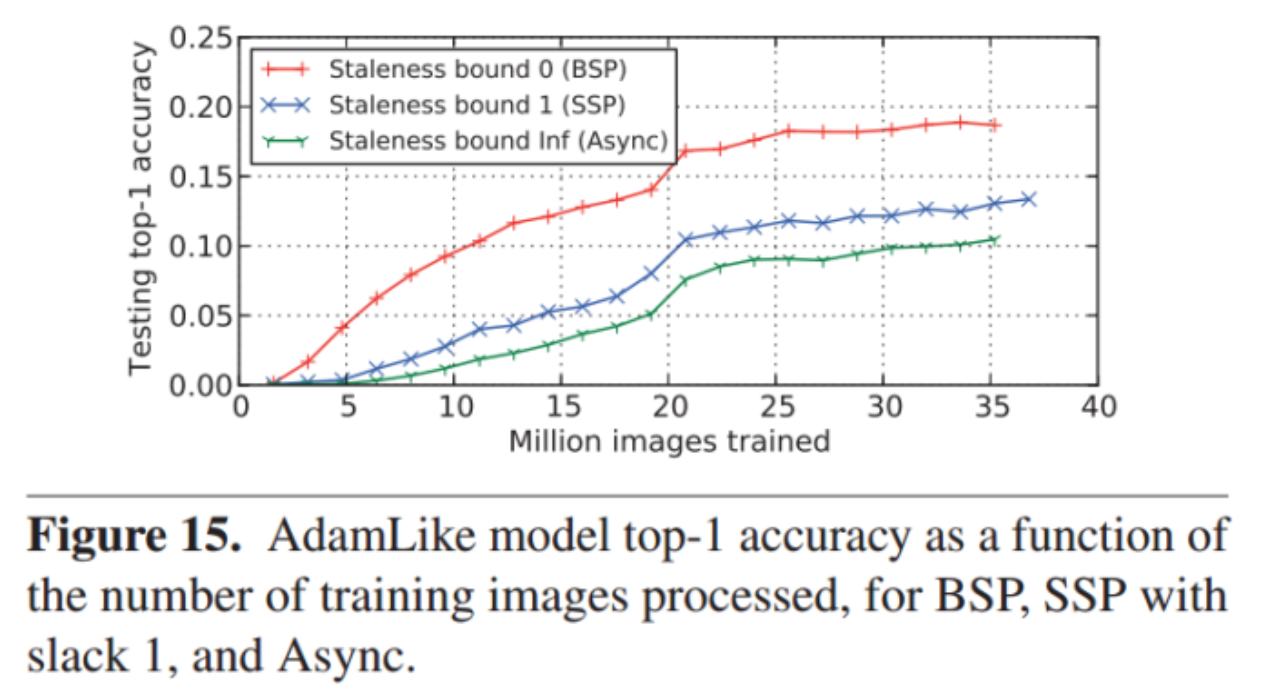
\includegraphics[width=0.85\textwidth]{asp-bsp-ssp}
\caption{ASP、BSP 以及 SSP 各同步策略对更新效率的影响}
\end{figure}

顺便提一句,考察分布式算法的性能,一般会分为 statistical performance 和 hard performance 来看。前者指不同的同步协议导致算法收敛需要的迭代次数的多少,
后者是单次迭代所对应的耗时。两者的关系和 precision/recall 关系类似,就不赘述了。有了 SSP,BSP 就可以通过指定 s=0 而得到。而 ASP 同样可以通过指定
s=$\infty$ 来达到。

\subsection{核心技术}\label{subsec:ps-cores}

除了参数服务器的架构、同步协议之外,本节再对其他技术做一个简要的介绍,详细的了解请直接阅读沐帅的博士论文和相关发表的论文% TODO
\footnote{http://www.cs.cmu.edu/\~muli/}。

热备、冷备技术:为了防止 server node 挂掉,导致任务中断,可以采用两个技术,一个是对参数分片进行热备,每个分片存储在三个不同的 server node 中,以 master-slave 的形式存活。如果 master 挂掉,可以快速从 slave 获取并重启相关 task。除了热备,还可以定时写入 checkpoint 文件到分布式文件系统来对参数分片及其状态进行备份。
进一步保证其安全性。

server node 管理:可以使用一致性哈希技术来解决 server node 的加入和退出问题,如图所示 
%% TODO 一致性哈希的方法,可以整理到第三章中,分布式系统中需要考虑的几个要素

\begin{figure}[hbtp]
\centering
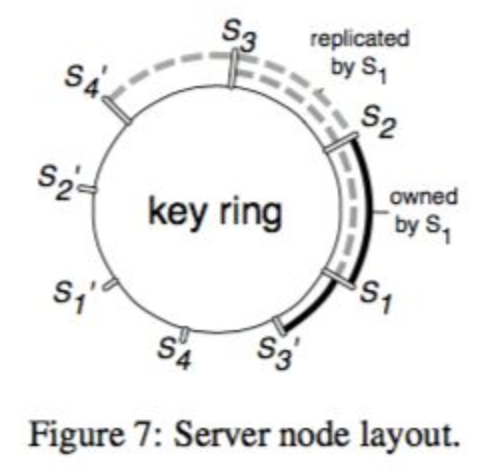
\includegraphics[width=0.65\textwidth]{server-node-layout}
\caption{Server node layout}
\end{figure}

当有 server node 加入或退出的时候,server manager 负责对参数进行重新分片或者合并。注意在对参数进行分片管理的情况下,一个分片只需要一把锁,
这大大提升了系统的性能,也是参数服务器可以实用的一个关键点。


\noindent\rule[0.25\baselineskip]{\textwidth}{1pt}

\section{大规模机器学习的四重境界}\label{sec:three-of-four}

到这里可以回到我们的标题了,大规模机器学习的四重境界到底是什么呢?这四重境界的划分是作者个人阅读总结的一种想法,并不是业界标准,仅供大家参考。

\subsection{境界 1}\label{subsec:first}

\noindent\textbf{参数可单机存储和更新}

此种境界较为简单,但仍可以使用参数服务器,通过数据并行来加速模型的训练。

\subsection{境界 2}\label{subsec:second}

\noindent\textbf{参数不可单机存储,可以单机更新}

此种情况对应的是一些简单模型,比如 sparse logistic regression;当 feature 的数量突破百亿的时候,LR 的权重参数
不太可能在一台机器上完全存下,此时必须使用参数服务器架构对模型参数进行分片。但是注意一点,SGD 的更新公式

\begin{equation*}
w^{\rq} = w - \alpha
\end{equation*}

其中可以分开到单个维度进行计算,但是单个维度的 $w_i = f(x)x_i$。

这里的 $f(w)$ 表示是全部参数 w 的一个函数,具体推导比较简单,这里篇幅所限就不赘述了。只是想说明 worker 在计算梯度的时候可能需要使用到
上一轮迭代的所有参数。而我们之所以对参数进行分片就是因为我们无法将所有参数存放到一台机器,现在单个 worker 有需要使用所有的参数
才能计算某个参数分片的梯度,这不是矛盾吗?可能吗?

答案是可能的,因为单个样本的 feature 具有很高的稀疏性(sparseness)。例如一个百亿 feature 的模型,单个训练样本往往只在其中很小
一部分 feature 上有取值,其他都为 0(假设 feature 取值都已经离散化了)。因此计算 $f(w)$ 的时候可以只拉取不为 0 的 feature 对应的
那部分 w 即可。有文章统计一般这个级别的系统,稀疏性往往在0.1\%(or 0.01\%,记得不是很准,大致这样)以下。这样的稀疏性,
可以让单机没有任何阻碍的计算 $f(w)$。

目前腾讯开源的 Angel 和 AILab 正在做的系统都处于这个境界。而原生 Spark 还没有达到这个境界,只能在中小规模的圈子里厮混。

\subsection{境界 3}\label{subsec:third}

\noindent\textbf{参数不可单机存储,不可单机更新,但无需模型并行}

境界 3 顺延境界 2 而来,当百亿级 feature 且 feature 比较稠密的时候,就需要计算框架进入到这层境界了,此时单个 worker 的能力有限,
无法完整加载一个样本,也无法完整计算 $f(w)$。怎么办呢?其实很简单,学过线性代数的都知道,矩阵可以分块。向量是最简单的矩阵,自然可以切成
一段一段的来计算。只是调度器需要支持算符分段而已了。

\subsection{境界 4}\label{subsec:fourth}

\noindent\textbf{参数不可单机存储,不可单机更新,需要模型并行}

进入到这个层次的计算框架,可以算是世界一流了。可以处理超大规模的神经网络。这也是最典型的应用场景。此时不仅模型的参数不能单机存储,
而且同一个迭代内,模型参数之间还有强的依赖关系,可以参见姐夫对 Distbelief 的介绍里的模型切分。

此时首先需要增加一个 coordinator 组件来进行模型并行的 concurrent 控制。同时参数服务器框架需要支持 namespace 切分,coordinator
将依赖关系通过 namespace 来进行表示。

一般参数间的依赖关系因模型而已,所以较难抽象出通用的 coordinator 来,而必须以某种形式通过脚本 parser 来生产整个计算任务的 DAG 图,然后通过 DAG 调度器来完成。对这个问题的介绍可以参考Erix Xing的分享\footnote{https://www.jianshu.com/p/00736aa21dc8}。

\subsection{TensorFlow}\label{subsec:tensorflow}

目前业界比较知名的深度学习框架有 Caffe、MXNet、Torch、Keras、Theano等,但目前最炙手可热的应该是 Google 发布的 TensorFlow。这里单独拿出来稍微分解下。

前面不少图片引自此文%
\footnote{TensorFlow:Large-Scale Machine Learning on Heterogeneous Distributed Systems}%
,从 TF 的论文来看,TF 框架本身是支持模型并行和数据并行的,内置了一个参数服务器模块,但从开源版本所曝光的 API 来看,TF 无法用来 10B 级别 feature
的稀疏 LR 模型。原因是已经曝光的 API 只支持在神经网络的不同层和层间进行参数切分,而超大规模 LR 可以看做一个神经单元,TF 不支持单个神经单元参数
切分到多个参数服务器 node 上。

当然,以 Google 的实力,绝对是可以做到第四重境界的,之所以没有曝光,可能是基于其他商业目的的考量,比如使用他们的云计算服务。

综上,个人认为如果能做到第四重境界,目前可以说的上是世界一流的大规模机器学习框架。仅从沐帅的 ppt 里看他曾经达到过,Google 内部应该也是没有问题的。
第三重境界应该是国内一流,第二充应该是国内前列吧。


\section{其他}\label{sec:other}

\subsection{资源管理}\label{subsec:resource-management}

本文没有涉及到的部分是资源管理,大规模机器学习框架部署的集群往往资源消耗也比较大,需要专门的资源管理工具来维护。这方面 yarn 和 mesos 都是佼佼者,
细节这里也就不介绍了

\subsection{设备}\label{subsec:devices}

除了资源管理工具,本身部署大规模机器学习集群本身对硬件也还是有些要求的,虽然理论上来说,所有 commodity 机器都可以用来搭建这类集群,但是考虑到性能,
我们建议尽量用高内存的机器+万兆及以上的网卡。没有超快速的网卡,玩参数传递和样本加载估计会比较苦逼。


\section{结语}\label{sec:another}

从后台转算法以来,长期沉浸于算法推理的论文无法自拔,对自己之前的后台工程能力渐渐轻视起来,觉得工程对算法的帮助不大。直到最近一个契机,
需要做一个这方面的调研,才豁然发现,之前的工程经验对我理解大规模机器学习框架非常有用,果然如李宗盛所说,人生每一步路,都不是白走的。

在一个月左右的调研中,脑子每天都充斥这各种疑问和困惑,曾经半夜4点醒来,思考同步机制而再也睡不着,干脆起来躲卫生间看书,而那天我一点多才睡。
当脑子里有放不下的问题的时候,整个人会处于一种非常亢奋的状态,除非彻底想清楚这个问题,否则失眠是必然的,上一次这种状态已经是很多年前了。
好在最后我总算理清了这方面的所有关键细节。以此,记之。Carbonzhang 于 2017 年 8 月 26 日凌晨!


\section*{致谢}

感谢 wills、janwang、joey、roberty、suzi 等同学一起讨论,特别感谢 burness 在 TF 方面的深厚造诣和调研。因为本人水平所限,错漏难免,
另外还有相当多的细节因为篇幅限制并未一一展开,仅仅是从较高抽象层面上简述了下大规模机器学习框架的关键思路,其他如分片向量锁、通信协议、时钟逻辑、
DAG 调度器、资源调度模块等均为展开来讲,希望以后有机会能补上。

\endinput

\chapter{分布式系统论文阅读}\label{chap:papers}
\addtocontents{los}{\protect\addvspace{10pt}}

\begin{intro}
整理阅读的分布式系统以及大数据处理方面的论文。
\end{intro}


\section{论文阅读要求}\label{sec:suggestions}

Cornell University CS6453%
\footnote{http://www.cs.cornell.edu/courses/cs6453/2017sp/index.html}%
给的阅读 paper 和准备 presentation 的建议

\textbf{Paper Reviews:} Please write constructive reviews. Here is a rough outline.
\begin{itemize}
	\item Summary of problem being solved (1-2 lines)
	\item Why is the problem interesting? Perhaps, its a new problem? Perhaps, its an old problem but with a new twist (e.g., new workloads, new environment, new hardware)? Perhaps, its just an old classical problem? (1-2 lines)
	\item What are the main insights in the proposed solution? What is the main technical contribution? How does the solution advance the state-of-the-art? (4-5 lines)
	\item Can you think of cases where the proposed solution may not work well? (4-5 lines)
	\item What are the next few problems that you would solve in this space? What do you think is the holy grail in this direction? (5-10 lines)
\end{itemize}

\textbf{Paper Presentations:} Please plan for 30 minutes. Here is a rough outline.
\begin{itemize}
	\item What is the problem being solved? (2-3 slides)
	\item Why is the problem interesting? Perhaps, its a new problem? Perhaps, its an old problem but with a new twist (e.g., new workloads, new environment, new hardware)? Perhaps, its just an old classical problem? (1-2 slides)
	\item What is the most related work and how is this paper different? (3-4 slides)
	\item What is the main technical contribution? What are the main insights used to build the proposed solution? How does the solution advance the state-of-the-art? (2-3 slides)
	\item Techniques used in the paper to solve the problem (4-5 slides)
	\item Can you think of cases where the proposed solution may not work well? (2-3 slides)
	\item What are the next few problems that you would solve in this space? What do you think is the holy grail in this direction? (4-5 slides)
\end{itemize}

所选择阅读并记录的论文参考自 Cornell CS6453 Spring2017%
\footnote{http://www.cs.cornell.edu/courses/cs6453/2017sp/schedule.html}%
和 MIT 6.824 Spring2018%
\footnote{https://pdos.csail.mit.edu/6.824/schedule.html}%

%
% 将各论文进行一个大的分类,在同一个 section 下
% 各论文讨论的东西作为 subsection 下
% 记录下阅读论文每个部分以及重读的时间,使用 【】 进行标记
%


\section{分布式存储}\label{sec:papers:storage}

\subsection{GFS}\label{paper:gfs}

\begin{itemize}
	\item [-] \textbf{The Google File System}
\end{itemize}

\begin{itemize}
	\item 【20180707】阅读了 Abstract \& Introduction 部分
	\item 
\end{itemize}

2003 年 Google 发表这篇论文,文中详细介绍了 Google 使用的分布式文件系统,其支持大规模分布式的数据密集型应用。那时候的计算机硬件特别昂贵且性能很差
(相较于现在,性价比应该是很低的),因此需要特别关注错误容忍(容错性,Fault Tolerance),集群中的任何一个节点可能在任何一个时间点宕机。

GFS 吸取了在其之前的众多分布式文件系统的特性,包括性能、可扩展性、可靠性、可用性(performance, scalability, reliability, and availability),
同时也根据 Google 具体的应用负载(application workloads)和应用环境(technological environment)进行了适配,重新审视了
传统分布式文件系统设计上的选择(choices),并提出了不同的系统设计考量。
\begin{enumerate}
	\item 集群中的组件故障(failures)是正常情况。在部署的分布式集群环境中,使用了成百上千台廉价的机器作为存储节点,这些组件宕掉是很正常的情况,
	因此所构建的系统需要满足(每一点都需要在之后补充上): %% TODO 
	\begin{itemize}
		\item constant monitoring
		\item error detection
		\item fault tolerance
		\item automatic recovery
	\end{itemize}
	\item 存储的文件非常大,比如 TB、PB 级别的数据
	\item 文件极少更新,更确切地说,文件作为某些计算的数据读入,并且不时有额外的数据追加到文件尾部
	\item 将文件系统的 API 与应用程序协同设计,以增加整个系统的灵活性
\end{enumerate}

\begin{newnote}[GFS 中为实现容错做了哪些手段?]
待补充 %% TODO Assign 20180707
\end{newnote}


\section{分布式计算}\label{sec:papers:computing}


\subsection{MapReduce}\label{paper:mapreduce}

\begin{itemize}
	\item [-] \textbf{MapReduce: Simplified Data Processing on Large Clusters}
\end{itemize}

\begin{itemize}
	\item %阅读 【20180707】
	\item 
\end{itemize}




\subsection{Spark}\label{paper:spark-and-rdd}

\begin{itemize}
	\item [-] \textbf{Spark: Cluster Computing with Working Sets}
	\item [-] \textbf{Resilient Distributed Datasets: A Fault-Tolerant Abstraction for In-Memory Cluster Computing}
\end{itemize}

\begin{itemize}
	\item %阅读 【20180707】 BSP
	\item 
\end{itemize}



\section{参数服务器}\label{sec:papers:ps}

\subsection{ASP}\label{paper:asp}

\begin{itemize}
	\item [-] \textbf{An Architecture for Parallel Topic Models}
\end{itemize}

\begin{itemize}
	\item %阅读 【20180707】
	\item 
\end{itemize}

2010 年的一篇文章,提出了参数服务器的概念,比较有开创性。

\subsection{SSP}\label{paper:ssp}

\begin{itemize}
	\item [-] \textbf{More Effective Distributed ML via a Stale Synchronous Parallel Parameter Server}
\end{itemize}

\begin{itemize}
	\item 【20180703】全文阅读,但跳过收敛性证明
	\item 【20180707】重读 \& 整理,同样跳过收敛性证明
\end{itemize}

这是分布式机器学习一个里程碑式的文章,提出了一个很 generic 的算法,提供了在某些合理假设下的收敛性证明(优化),并且在这个基础上
提出了一个合理的编程模型,最后给了一个系统实现。%
\footnote{https://zhuanlan.zhihu.com/p/29032307}%

在 Spark/Hadoop 中每个 worker 的新一次迭代都需要等待所有 workers 上一次迭代的结束,要用到上一次迭代的结果(BSP);
而对于 ASP,每一个 worker 执行调度器分配给自己的那部分任务,不用等待其他 workers 的执行。一个很直接的想法就是能否寻找一个折衷的
同步策略,即不是像 BSP 那样每次迭代都强制所有 workers 对上一次迭代进行同步,也不是像 ASP 那样各 workers 随意执行,而是每个 worker
都按照自己的节奏执行程序,但要求执行最快的那个 worker 与执行最慢的那个 worker 之间不能超过所指定的迭代数,例如 3 个迭代,如图
\ref{fig:paper-ssp} 所示。 

\begin{figure}[hbtp]
\centering
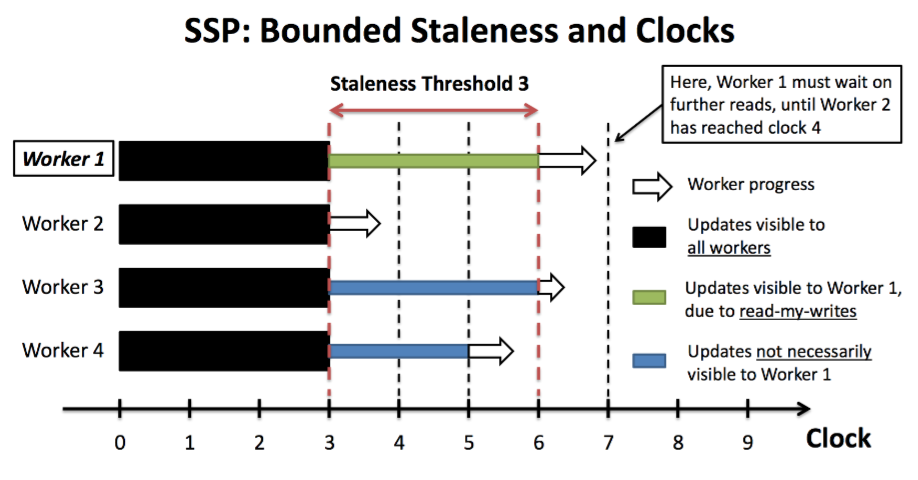
\includegraphics[width=0.65\textwidth]{paper-ssp}
\caption{SSP 模型示例}
\label{fig:paper-ssp}
\end{figure}

\begin{newnote}[摘录 SSP 论文中的描述]
We begin with an informal explanation of SSP: assume a collection of $P$ workers, each of which makes
additive updates to a shared parameter $x \gets x + \mu$ at regular intervals called \textit{clocks}.
Clocks are similar to iterations, and represent some unit of progress by an ML algorithm. Every worker
has its own integer-valued clock $c$, and workers only commit their updates at the end of each clock.
Updates may not be immediately visible to other workers trying to read $x$ --- in other words, workers
only see effects from a “stale” subset of updates. The idea is that, with staleness, workers can retrieve
updates from caches on the same machine (fast) instead of querying the parameter server over
the network (slow). Given a user-chosen staleness threshold $s \ge 0$, SSP enforces the following
bounded staleness conditions:

\begin{itemize}
	\item The slowest and fastest workers must be $\le s$ clocks apart --- otherwise, the fastest worker
	is forced to wait for the slowest worker to catch up.
	\item When a worker with clock $c$ commits an update $\mu$, that $\mu$ is timestamped with time $c$.
	\item When a worker with clock $c$ reads $x$, it will always see effects from all $\mu$ with timestamp
	$\le c - s - 1$. It may also see some $\mu$ with timestamp $> c - s - 1$ from other workers.
	\item Read-my-writes: A worker $p$ will always see the effects of its own updates up.
\end{itemize}
\end{newnote}


\subsection{Parameter Server}\label{paper:ps-osdi2014}

% http://chuansong.me/n/2161528 参数服务器——分布式机器学习的新杀器

\begin{itemize}
	\item [-] \textbf{Scaling Distributed Machine Learning with the Parameter Server}
	\item [-] \textbf{Communication Efficient Distributed Machine Learning with the Parameter Server}
\end{itemize}

\begin{itemize}
	\item 【20180625】阅读过好几遍了,打印纸质版、MarginNote 上,在笔记上手写了笔记
	\item 【20180707】重读 \& 整理
	\item 【20180708】整理,差论文 2.2 3.4 的理解与整理,可能需要看过 ps-lite 代码之后才能理解的更清晰
\end{itemize}

沐帅在 OSDI 2014 上发表这篇工作,引出第三代参数服务器框架,在 worker 节点上分布式存放数据和工作负载,server 节点上保存着
全局共享的参数,各节点之间异步通信,支持灵活的一致性模型,可扩展并且容错性很好(continuous fault tolerance 是什么意思)。

当处理大规模的机器学习(深度学习)模型时,会面临这样一个问题:多台机器节点之间需要共享一些状态信息,包括参数、集群信息,用户 profiles
以及其他一些需要在各节点之间进行交流的信息。另外,单机已经解决不了目前快速增长的数据和参数了,在实际的系统中训练的数据量已经达到 TB、PB
级别,训练过程中可能会产生 $10^9 \sim 10^{12}$ 的参数量(这两个数据是在 2014 年年初时候的数据,现在需要更新了)。%% TODO
模型参数被所有的 worker 节点所共享并且会被频繁访问到,这就会带来很多问题和挑战:
\begin{enumerate}
	\item 访问这些巨量的参数,需要大量的网络带宽支持
	\item 很多机器学习算法是连续型的(顺序的),只有上一次迭代完成(各个 worker 上都完成)之后,才能进行下一次迭代,这导致如果
	各机器之间的性能差距太大(木桶效应),就会造成性能的极大损失(因为系统整体的性能由性能最差的那台机器所决定)
	\item 在分布式系统中容错能力是非常重要的,在真实环境的部署下,算法最终是在云上(云计算)运行的(这种环境下,机器是不可靠的,
	并且所提交的 job 可能会被其他任务抢占)
\end{enumerate}

沐帅将参数服务器的发展分为三个阶段:
\begin{itemize}
	\item [第一代] 缺少灵活性和性能 --- 仅使用 memcached 分布式 (key, value) 存储,来作为同步机制。YahooLDA
	通过改进这一机制,增加了一个专门的服务器,提供用户能够自定义的更新操作(set/get/update)
	\item [第二代] Petuum 使用 bounded delay 模型来改进 YahooLDA,但是却限制了 worker 的线程模型
	\item [第三代] 即在这篇 paper 中提出来,能够解决这些局限性
\end{itemize}

参数服务器与通用的分布式系统有什么区别呢?通用的分布式系统通常是每次迭代都强制同步,在十几个节点上它们的性能可以表现的很好,但是
在大规模集群中,这样的每次迭代强制同步的机制(BSP)会因为木桶效应变得很慢。Mahout 基于 Hadoop,MLI 基于 Spark,它们
(MLI 和 Spark)采用的都是 Iterative MapReduce 架构,能够保持迭代之间的状态,并且执行策略也更加优化了,但是由于这两种方法
均采用了同步迭代的通信方式,使得它们很容易因为个别机器的低性能导致全局性能的降低。为了解决这个问题,GraphLab 采用图形抽象的方式
进行异步通信,但是它缺少以 MapReduce 为基础架构的弹性扩展性,并且它使用粗粒度的 snapshots 来进行恢复,这两点都会阻碍到可扩展性。

参数服务器正是吸取了两者的优点,1)MLI 和 Spark 保持各个迭代之间的状态信息,2)GraphLab 异步通信,并且解决了 GraphLab 在
可扩展性方面的劣势。

\noindent\textbf{Distributed Subgradient Descent} 论文的 2.2 节 %% TODO 待整理

\noindent\textbf{架构}

一个参数服务器的实例可以同时运行多个算法。参数服务器的节点以 group 进行分组,包含一个 server group 和多个 worker group,
如图 \ref{fig:paper-ps-architecture} 所示。

\begin{figure}[hbtp]
\centering
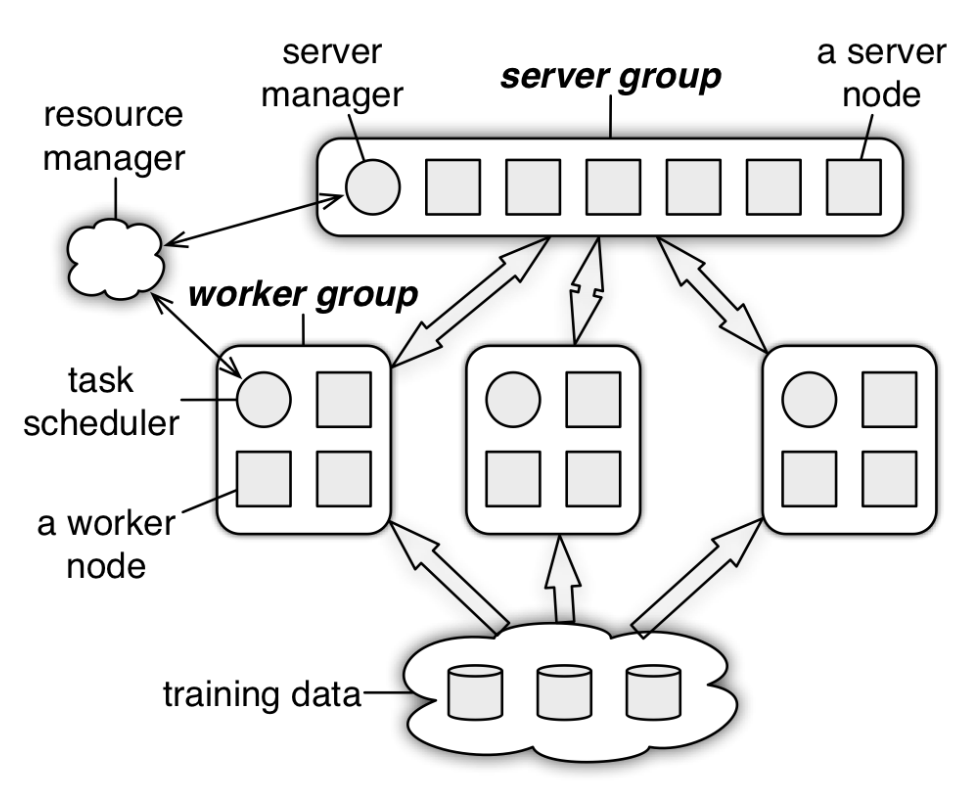
\includegraphics[width=0.65\textwidth]{paper-ps-architecture}
\caption{参数服务器的架构}
\label{fig:paper-ps-architecture}
\end{figure}

在 server group 中的每一个 server 节点保存着部分全局共享的参数,每个 server 节点之间会进行通信,以进行备份或者迁移节点上的参数,
这是为了整个系统的容错性和可扩展性考虑。在 server group 中有一个节点的角色是 server manager,保存各 server 节点的元数据信息
(包括节点是否存活,分配在其上的共享参数的范围),需要考虑如何保持一致性。

每一个 worker group 上都运行着一个应用。每一个 worker 节点上都本地保存着部分的训练数据,用来计算一个本地的梯度值。worker 节点
将计算得到的梯度值 push 给 server 节点,或者从 server 节点上 pull 下已更新的参数;各 worker 节点之间不进行通信。每一个 worker
group 中同样有一个 task scheduler 节点,负责分配任务给 group 中的所有 worker 节点,并监测各 worker 的执行进度,在新的 worker
节点添加进该 group 或有 worker 节点被移除时,scheduler 节点负责重新调度未完成的任务。

参数服务器支持独立的参数命名空间(namespace)。

沐帅提出的第三代参数服务器包含以下几个要点:
\begin{itemize}
	\item 所有共享参数的形式都是 (key, value) vectors --- 假设 keys 是有序的,不存在的 key 对应的 value 值为 0
	\item 基于 range 的 push/pull 操作,这样 worker 节点每次与 server 节点进行通信时可以选择性的仅传递少量需要更新的参数,
	更可控也更灵活
	\item server 节点用于聚集各 worker 节点发送过来的各子梯度值,同时,server 节点也支持执行用户指定的操作。支持这样的操作是很有
	好处的,因为 server 节点通常保存有更完整并且更 up-to-date 的共享参数信息
	\item 异步操作,回调的实现 %% TODO
	\item 各 worker 节点异步的执行任务,各节点之间可能会出现数据不一致,从而使得算法的收敛过程变慢。然而,有一些算法对数据的一致性
	要求没有那么严格,即有一些算法在数据出现不一致时,也能够在最终收敛并得到准确的结果。

	对一致性协议的考量,需要在系统性能跟算法收敛速率之间做一个 tradeoff,同时考虑:
	\begin{enumerate}
		\item 算法对于参数非一致性的敏感程度
		\item 训练数据的特征之间的关联度
		\item 硬件设备的能力
	\end{enumerate}

	考虑到用户使用的时候会有不同的情况,参数服务器为用户提供了多种任务依赖方式,1)Sequential,2)Eventual,3)Bounded delay
	\item 用户可自定义的过滤器。对于机器学习优化问题来说,比如梯度下降,并不是每次计算的梯度对于最终优化都是有价值的,用户可以通过
	自定义的规则过滤一些不必要的通信,再进一步压缩带宽耗费:
	\begin{enumerate}
		\item 发送很小的梯度值是低效的 --- 因此可以自定义设置,只在梯度值很大的时候发送
		\item 更新接近最优情况的值是低效的 --- 因此只在非最优情况下发送,可通过 KKT 条件来判断
	\end{enumerate}
\end{itemize}

%% 待补充什么呢?


\subsection{GeePS}\label{paper:geeps}

\begin{itemize}
	\item [-] \textbf{GeePS: Scalable deep learning on distributed GPUs with a GPU-specialized parameter server}
\end{itemize}

\begin{itemize}
	\item %【20180707】阅读
	\item 
\end{itemize}



% \section{}\label{sec:papers:}

% \subsection{}\label{}

% \subsection{}\label{}

% \subsection{}\label{}


\endinput

\chapter{深度学习框架}\label{chap:framework}
\addtocontents{los}{\protect\addvspace{10pt}}

\begin{intro}
本章内容主要是对博客\textbf{The Anatomy of Deep Learning Frameworks}%
\footnote{https://medium.com/@gokul\_uf/the-anatomy-of-deep-learning-frameworks-46e2a7af5e47}%
的总结与整理。

可以考虑看看这个课程 CSE 599W: Systems for ML%
\footnote{http://dlsys.cs.washington.edu/}%
\end{intro}

许多初学者觉得深度学习框架抽象,虽然调用了几个函数/方法,计算了几个数学难题,
但始终不能理解这些框架的全貌。

为了更好地认识深度学习框架,也为了给一些想要自己亲手搭建深度学习框架的朋友提供
一些基础性的指导,日前来自苏黎世联邦理工学院计算机科学系的硕士研究生
Gokula Krishnan Santhanam在博客上撰文,概括了大部分深度学习框架都会包含
的五大核心组件,为我们详细剖析了深度学习框架一般性的内部组织结构。%
本文为雷锋网编译% TODO 在进行理解时,需要大量参考原英文博客,给了很多链接资料
\footnote{https://www.leiphone.com/news/201701/DZeAwe2qgx8JhbU8.html}%
。

Gokula Krishnan Santhanam认为,大部分深度学习框架都包含以下五个核心组件:
\begin{enumerate}
	\item 张量(Tensor)
	\item 基于张量的各种操作
	\item 计算图(Computation Graph)
	\item 自动微分工具(Automatic Differentiation)
	\item BLAS、cuBLAS、cuDNN 等扩展包
\end{enumerate}

\section{张量}\label{sec:tensor}

张量是所有深度学习框架中最核心的组件,因为后续的所有运算和优化算法都是基于张量进行的。
几何代数中定义的张量是基于向量和矩阵的推广,通俗一点理解的话,我们可以将标量视为零阶
张量,矢量视为一阶张量,那么矩阵就是二阶张量。

举例来说,我们可以将任意一张 RGB 彩色图片表示成一个三阶张量(三个维度分别是图片的高度、
宽度和色彩数据)。如图 \ref{} 所示,是一张普通的水果图片,按照 RGB 三原色表示,其
可以拆分为三张红色、绿色和蓝色的灰度图片,如果将这种表示方法用张量的形式写出来,就是
图中最下方的那张表格。

\begin{figure}[hbtp]
\centering
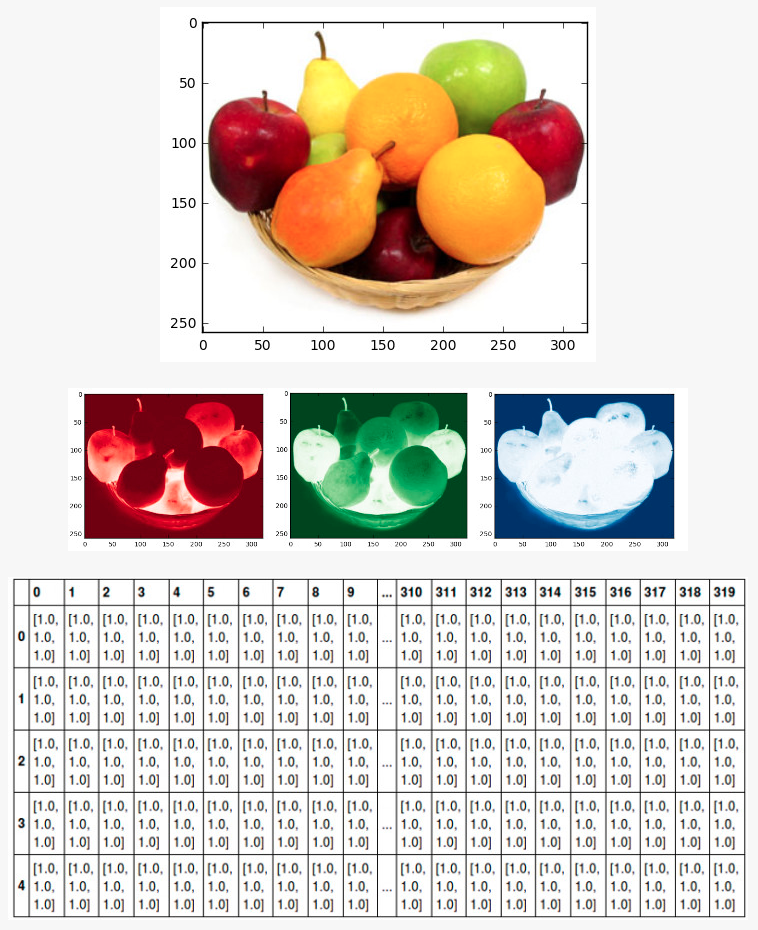
\includegraphics[width=0.45\textwidth]{framework-fruit-three-tensor}
\caption{水果的三种表示}
\label{fig:framework-fruit-three-tensor}
\end{figure}

图中只显示了前 5 行、320 列的数据,每个方格代表一个像素点,其中的数据 [1.0, 1.0, 1.0]
即为颜色。假设用[1.0, 0, 0]表示红色,[0, 1.0, 0]表示绿色,[0, 0, 1.0]表示蓝色,
那么前面5行的数据则全是白色。

将这一定义进行扩展,我们也可以用四阶张量表示一个包含多张图片的数据集,其中的四个维度分别是:
图片在数据集中的编号,图片高度、宽度,以及色彩数据。

将各种各样的数据抽象成张量表示,然后再输入神经网络模型进行后续处理是一种非常必要且高效的策略。
因为如果没有这一步骤,我们就需要根据各种不同类型的数据组织形式定义各种不同类型的数据操作,
这会浪费大量的开发者精力。更关键的是,当数据处理完成后,我们还可以方便地将张量再转换回
想要的格式。例如 Python Numpy 包中 numpy.imread 和 numpy.imsave 两个方法,分别
用来将图片转换成张量对象(即代码中的 Tensor 对象),和将张量再转换成图片保存起来。


\section{基于张量的各种操作}\label{sec:tensor-operations}

有了张量对象之后,下面一步就是一系列针对这一对象的数学运算和处理过程。如图 \ref{} 所示。

\begin{figure}[hbtp]
\centering
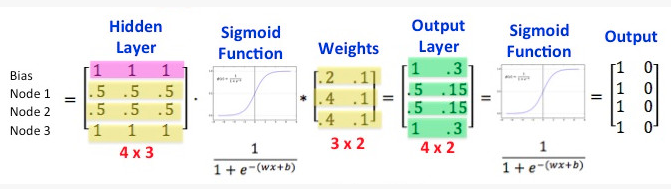
\includegraphics[width=0.85\textwidth]{framework-tensor-operations}
\caption{基于张量的各种操作}
\label{fig:framework-tensor-operations}
\end{figure}

其实,整个神经网络都可以简单视做为了达到某种目的,针对输入张量进行的一系列操作的过程。而所谓的
“学习”就是不断纠正神经网络的实际输出结果和预期结果之间误差的过程。这里的一系列操作包含的范围很宽,
可以是简单的矩阵乘法,也可以是卷积、池化和 LSTM 等稍复杂的运算。而且各框架支持的张量操作通常
也不尽相同,详细情况可以查看其官方文档。

需要指出的是,大部分的张量操作都是基于类实现的(而且是抽象类),而并不是函数(这一点可能要归功于
大部分的深度学习框架都是用面向对象的编程语言实现的)。这种实现思路一方面允许开发者将各种类似的操作
汇总在一起,方便组织管理。另一方面也保证了整个代码的复用性、扩展性和对外接口的统一。总体上让整个
框架更灵活和易于扩展,为将来的发展预留了空间。


\section{计算图}\label{sec:computation-graph}

有了张量和基于张量的各种操作之后,下一步就是将各种操作整合起来,输出我们需要的结果。

但不幸的是,随着操作种类和数量的增多,有可能引发各种意想不到的问题,包括多个操作之间应该并行还是
顺次执行,如何协同各种不同的底层设备,以及如何避免各种类型的冗余操作等等。这些问题有可能拉低整个
深度学习网络的运行效率或者引入不必要的Bug,而计算图正是为解决这一问题产生的。

计算图首次被引入人工智能领域是在 2009 年的论文《Learning Deep Architectures for AI》。
当时的示意图如下图 \ref{} 所示,作者用不同的占位符(*,+,sin)构成操作结点,以字母 x、a、b
构成变量结点,再以有向线段将这些结点连接起来,组成一个表征运算逻辑关系的清晰明了的“图”型数据结构,
这就是最初的计算图。

\begin{figure}[hbtp]
\centering
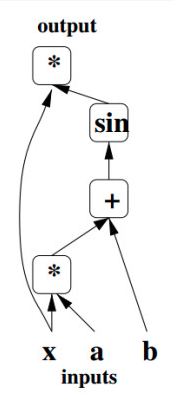
\includegraphics[width=0.25\textwidth]{framework-computation-graph}
\caption{最初的计算图}
\label{fig:framework-computation-graph}
\end{figure}

将计算图作为前后端之间的中间表示(Intermediate Representations)可以带来良好的交互性,
开发者可以将 Tensor 对象作为数据结构,函数/方法作为操作类型,将特定的操作类型应用于特定的
数据结构,从而定义出类似 MATLAB 的强大建模语言。

需要注意的是,通常情况下开发者不会将用于中间表示得到的计算图直接用于模型构造,因为这样的计算图
通常包含了大量的冗余求解目标,也没有提取共享变量,因而通常都会经过依赖性剪枝、符号融合、内存共享等
方法对计算图进行优化。

目前,各个框架对于计算图的实现机制和侧重点各不相同。例如 Theano 和 MXNet 都是以隐式处理的方式
在编译中由表达式向计算图过渡。而 Caffe 则比较直接,可以创建一个 Graph 对象,然后以类似
Graph.Operator(xxx) 的方式显示调用。

因为计算图的引入,开发者得以从宏观上俯瞰整个神经网络的内部结构,就好像编译器可以从整个代码的角度
决定如何分配寄存器那样,计算图也可以从宏观上决定代码运行时的 GPU 内存分配,以及分布式环境中不同
底层设备间的相互协作方式。除此之外,现在也有许多深度学习框架将计算图应用于模型调试,可以实时输出
当前某一操作类型的文本描述。


\section{自动微分工具}\label{sec:automatic-differentiation}

计算图带来的另一个好处是让模型训练阶段的梯度计算变得模块化且更为便捷,也就是自动微分法。

正如前面提到的,因为我们可以将神经网络视为由许多非线性过程组成的一个复杂的函数体,而计算图则以模块化
的方式完整表征了这一函数体的内部逻辑关系,因此微分这一复杂函数体,即求取模型梯度的方法就变成了在计算图
中简单地从输入到输出进行一次完整遍历的过程。与自动微分对应,业内更传统的做法是符号微分。

符号微分即常见的求导分析。针对一些非线性过程(如修正线性单元 ReLU)或者大规模的问题,使用符号微分法的
成本往往非常高昂,有时甚至不可行(即不可微)。因此,以上述迭代式的自动微分法求解模型梯度已经被广泛采用。
并且由于自动微分可以成功应对一些符号微分不适用的场景,目前许多计算图程序包
(例如Computation Graph Toolkit)都已经预先实现了自动微分。

另外,由于每个节点处的导数只能相对于其相邻节点计算,因此实现了自动微分的模块一般都可以直接加入任意的
操作类中,当然也可以被上层的微分大模块直接调用。


\section{BLAS/cuBLAS/cuDNN 等扩展包}\label{sec:blas-extension}

现在,通过上述所有模块,我们已经可以搭建一个全功能的深度学习框架:将待处理数据转换为张量,针对张量施加
各种需要的操作,通过自动微分对模型展开训练,然后得到输出结果开始测试。这时还缺什么呢?答案是运算效率。

由于此前的大部分实现都是基于高级语言的(如 Java、Python、Lua 等),而即使是执行最简单的操作,高级语言
也会比低级语言消耗更多的 CPU 周期,更何况是结构复杂的深度神经网络,因此运算缓慢就成了高级语言
的一个天然的缺陷。

目前针对这一问题有两种解决方案。

第一种方法是模拟传统的编译器。就好像传统编译器会把高级语言编译成特定平台的汇编语言实现高效运行一样,这种
方法将高级语言转换为 C 语言,然后在 C 语言基础上编译、执行。为了实现这种转换,每一种张量操作的实现代码
都会预先加入 C 语言的转换部分,然后由编译器在编译阶段将这些由 C 语言实现的张量操作综合在一起。目前
pyCUDA 和 Cython 等编译器都已经实现了这一功能。

第二种方法就是前文提到的,利用脚本语言实现前端建模,用低级语言如 C++ 实现后端运行,这意味着高级语言和
低级语言之间的交互都发生在框架内部,因此每次的后端变动都不需要修改前端,也不需要完整编译(只需要通过修改
编译参数进行部分编译),因此整体速度也就更快。

除此之外,由于低级语言的最优化编程难度很高,而且大部分的基础操作其实也都有公开的最优解决方案,因此另一个
显著的加速手段就是利用现成的扩展包。例如最初用 Fortran 实现的 BLAS(基础线性代数子程序),
就是一个非常优秀的基本矩阵(张量)运算库,此外还有英特尔的 MKL(Math Kernel Library)等,
开发者可以根据个人喜好灵活选择。

\begin{figure}[hbtp]
\centering
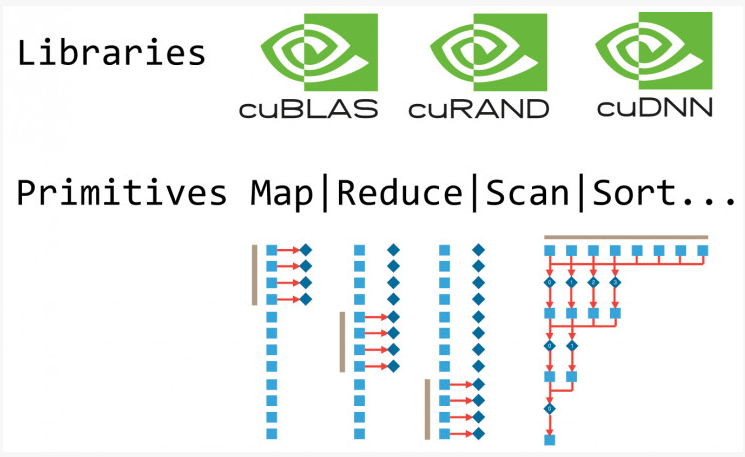
\includegraphics[width=0.5\textwidth]{framework-blas-extension}
\caption{BLAS/cuBLAS/cuDNN 等扩展包}
\label{fig:framework-blas-extension}
\end{figure}

值得一提的是,一般的 BLAS 库只是针对普通的 CPU 场景进行了优化,但目前大部分的深度学习模型都已经开始采用
并行 GPU 的运算模式,因此利用诸如 NVIDIA 推出的针对 GPU 优化的 cuBLAS 和 cuDNN 等更据针对性
的库可能是更好的选择。

运算速度对于深度学习框架来说至关重要,例如同样训练一个神经网络,不加速需要 4 天的时间,加速的话可能只要
4 小时。在快速发展的人工智能领域,特别是对那些成立不久的人工智能初创公司而言,这种差别可能就会决定谁是
先驱者,而谁是追随者。


\section{总结}\label{sec:framework-conclusion}

原文作者在文末指出:为了向开发者提供尽量简单的接口,大部分深度学习框架通常都会将普通的概念抽象化,这可能
是造成许多用户感知不到上述五点核心组件的重要原因。

而这也正是作者写本文的初衷:他希望开发者能够通过了解不同框架之间的一些相似特性,更好地认识和使用一个深度
学习框架。另一方面,对于那些不仅对学会使用深度学习框架感兴趣,还打算亲手搭建一个深度框架的朋友,作者认为
了解各框架的内部组成和一些共性的特征也是迈向成功的重要一步。他真诚地相信,一个优秀的工程师不仅应该
“知其然”,更应该“知其所以然”。


\endinput
\chapter{分布式系统的基本要素}\label{chap:distributed-system}
\addtocontents{los}{\protect\addvspace{10pt}}

\begin{intro}

\end{intro}

\section{Vector Clock}\label{sec:vector-clock}

\subsection{}

\subsection{}


\section{一致性哈希}\label{sec:consistent-hasing}

本节整理自博客『一致性哈希算法及其在分布式系统中的应用%
\footnote{http://blog.codinglabs.org/articles/consistent-hashing.html}%
』

本节将会从实际应用场景出发,介绍一致性哈希算法(Consistent Hashing)及其在分布式系统中的应用。首先本节会描述一个在日常开发中
经常会遇到的问题场景,借此介绍一致性哈希算法以及这个算法如何解决此问题;接下来会对这个算法进行相对详细的描述,并讨论一些如虚拟节点
等与此算法应用相关的话题。

\subsection{分布式缓存问题}

假设我们有一个网站,最近发现随着流量增加,服务器压力越来越大,之前直接读写数据库的方式不太给力了,于是我们想引入 Memcached
作为缓存机制。现在我们一共有三台机器可以作为 Memcached 服务器,如图 \ref{fig:system-memcached-deployment} 所示。

\begin{figure}[hbtp]
\centering
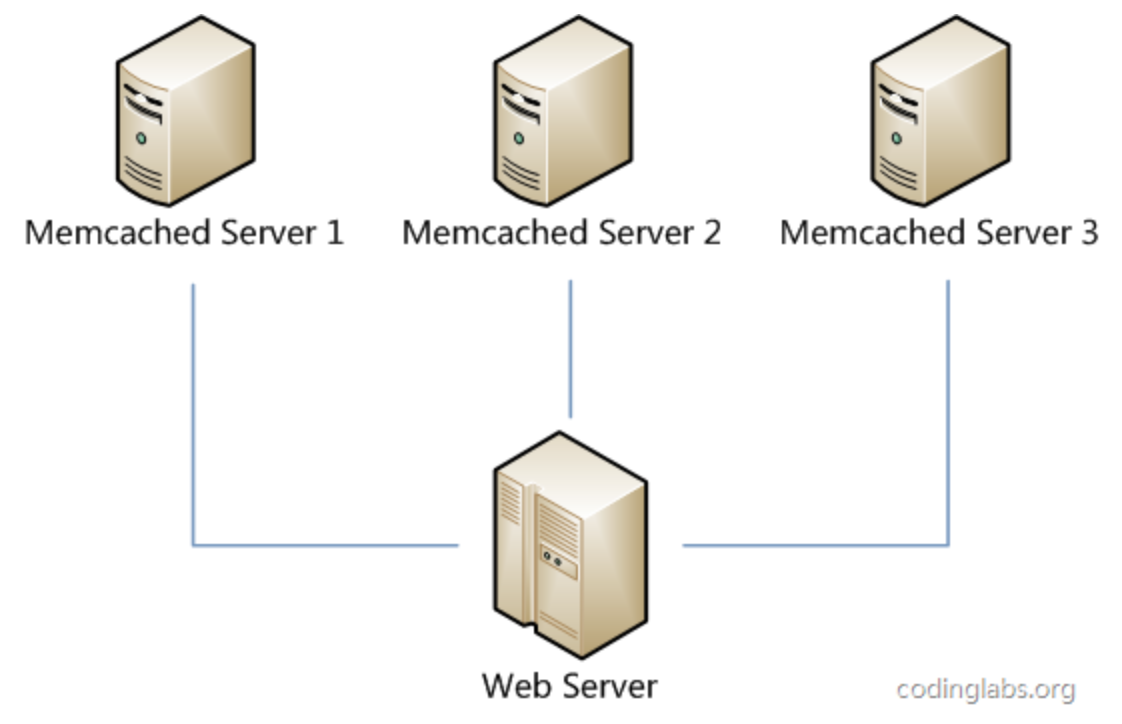
\includegraphics[width=0.45\textwidth]{system-memcached-deployment}
\caption{三台 Memcached 服务器}
\label{fig:system-memcached-deployment}
\end{figure}

很显然,最简单的策略是将每一次 Memcached 请求随机发送到一台 Memcached 服务器,但是这种策略可能会带来两个问题:
\begin{enumerate}
	\item 同一份数据可能被存在不同的机器上而造成数据冗余
	\item 有可能某数据已经被缓存但是访问却没有命中,因为无法保证对相同key的所有访问都被发送到相同的服务器
\end{enumerate}
因此,随机策略无论是时间效率还是空间效率都非常不好。

要解决上述问题只需做到如下一点:保证对相同 key 的访问会被发送到相同的服务器。很多方法可以实现这一点,最常用的方法是计算哈希。
例如对于每次访问,可以按如下算法计算其哈希值:
\begin{equation*}
h = Hash(key) \% 3
\end{equation*}
其中,Hash 是一个从字符串到正整数的哈希映射函数。这样,如果我们将 Memcached Server 分别编号为 0、1、2,那么就可以根据上式和
key 计算出服务器编号 h,然后去访问。

这个方法虽然解决了上面提到的两个问题,但是存在一些其它的问题。如果将上述方法抽象,可以认为通过:
\begin{equation*}
h = Hash(key) \% N
\end{equation*}
这个算式计算每个 key 的请求应该被发送到哪台服务器,其中,N 为服务器的台数,并且服务器按照 0 $\sim$ (N-1) 编号。这个算法的问题在于
容错性和扩展性不好。所谓容错性是指当系统中某一个或几个服务器变得不可用时,整个系统是否可以正确高效运行;而扩展性是指当加入新的
服务器后,整个系统是否可以正确高效运行。

现假设有一台服务器宕机了,那么为了填补空缺,要将宕机的服务器从编号列表中移除,后面的服务器按顺序前移一位并将其编号值减一,
此时每个 key 就要按 $h = Hash(key) \% (N-1)$ 重新计算;同样,如果新增了一台服务器,虽然原有服务器编号不用改变,但是
要按$h = Hash(key) \% (N+1)$重新计算哈希值。因此系统中一旦有服务器变更,大量的 key 会被重定位到不同的服务器从而造成大量的
缓存不命中。而这种情况在分布式系统中是非常糟糕的。

一个设计良好的分布式哈希方案应该具有良好的单调性,即服务节点的增减不会造成大量哈希重定位。一致性哈希算法就是这样一种哈希方案。


\subsection{一致性哈希算法}

\noindent\textbf{算法简述}

一致性哈希算法(Consistent Hashing)最早在这篇论文%
\footnote{Consistent Hashing and Random Trees: Distributed Caching Protocols for Relieving Hot Spots on the World Wide Web}%
中提出。简单来说,一致性哈希将整个哈希值空间组织成一个虚拟的圆环,如假设某哈希函数 H 的值空间为 $0 \sim 2^{32}-1$
(即哈希值是一个 32 位无符号整形),整个哈希空间环如图 \ref{fig:system-hashing-ring-1} 所示。
\begin{figure}[hbtp]
\centering
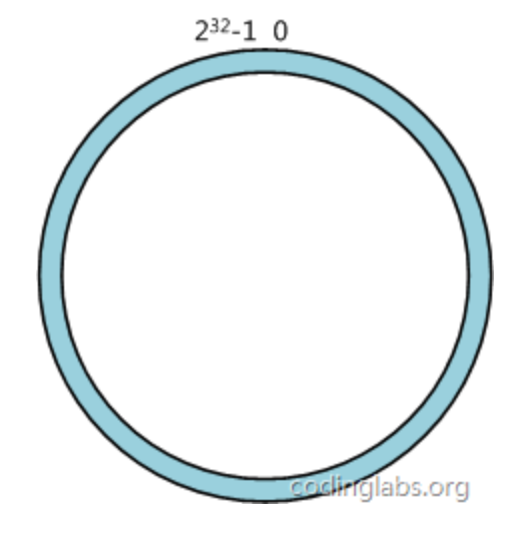
\includegraphics[width=0.3\textwidth]{system-hashing-ring-1}
\caption{哈希空间环}
\label{fig:system-hashing-ring-1}
\end{figure}
整个空间按顺时针方向组织。0 和 $2^{32}-1$ 在零点中方向重合。

下一步将各个服务器使用 H 进行一个哈希,具体可以选择服务器的 ip 或主机名作为关键字进行哈希,这样每台机器就能确定其在哈希环上的位置,
这里假设将上文中三台服务器使用 ip 地址哈希后在环空间的位置如图 \ref{fig:system-hashing-ring-2} 所示

\begin{figure}[hbtp]
\centering
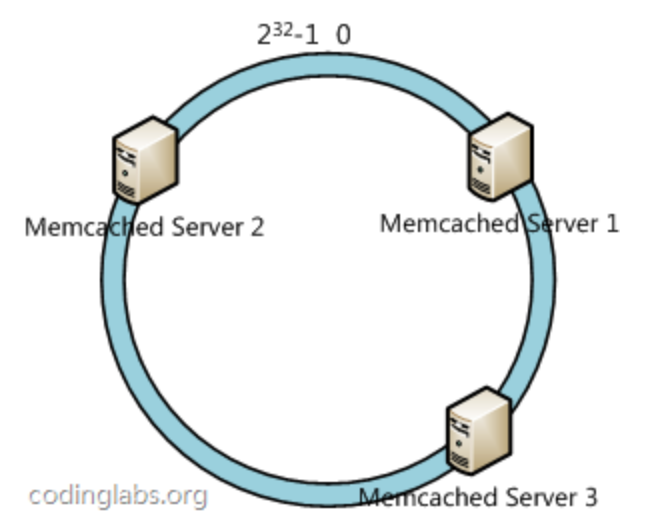
\includegraphics[width=0.3\textwidth]{system-hashing-ring-2}
\caption{三台服务器映射到哈希环上的位置}
\label{fig:system-hashing-ring-2}
\end{figure}

接下来使用如下算法定位数据访问到相应服务器:将数据 key 使用相同的函数 H 计算出哈希值 h,根据 h 确定此数据在环上的位置,从此位置
沿环顺时针『行走』,第一台遇到的服务器就是其应该定位到的服务器。

例如我们有 A、B、C、D 四个数据对象,经过哈希计算后,在环空间上的位置如图 \ref{fig:system-hashing-ring-3}

\begin{figure}[hbtp]
\centering
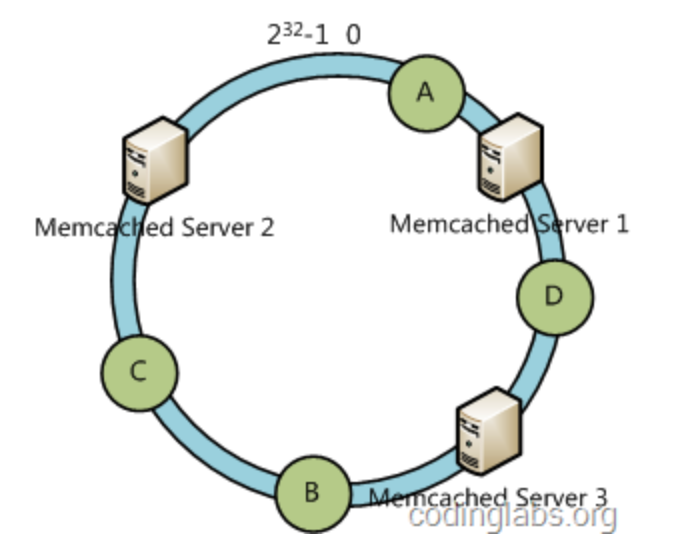
\includegraphics[width=0.3\textwidth]{system-hashing-ring-3}
\caption{四个数据对象映射到哈希环上的位置}
\label{fig:system-hashing-ring-3}
\end{figure}

根据一致性哈希算法,数据 A 会被定位到 Server 1 上,D 被定为到 Server 3 上,而 B、C 分别被定为到 Server 2 上。

\noindent\textbf{容错性与可扩展性分析}

下面分析一致性哈希算法的容错性和可扩展性。现假设 Server 3 宕机了:

\begin{figure}[hbtp]
\centering
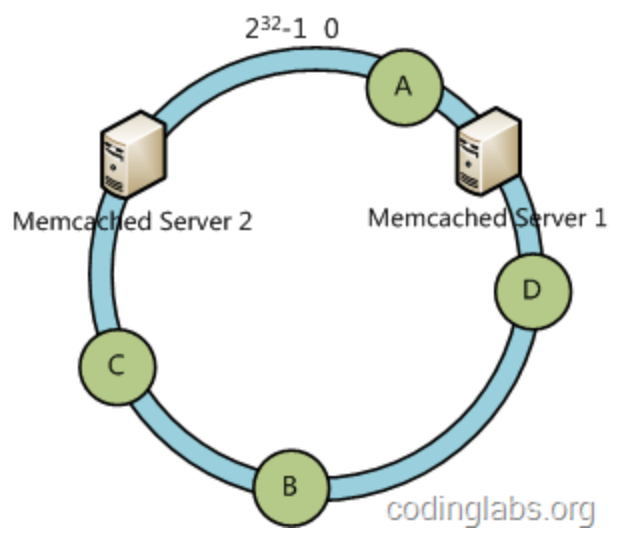
\includegraphics[width=0.3\textwidth]{system-hashing-ring-4}
\caption{Server3宕机}
\label{fig:system-hashing-ring-4}
\end{figure}

可以看到此时 A、C、B 不会受到影响,只有 D 节点被重定位到 Server 2。一般的,在一致性哈希算法中,如果一台服务器不可用,
则受影响的数据仅仅是此服务器到其环空间中前一台服务器(即顺着逆时针方向行走遇到的第一台服务器)之间数据,其它不会受到影响。

下面考虑另外一种情况,如果我们在系统中增加一台服务器 Memcached Server 4:

\begin{figure}[hbtp]
\centering
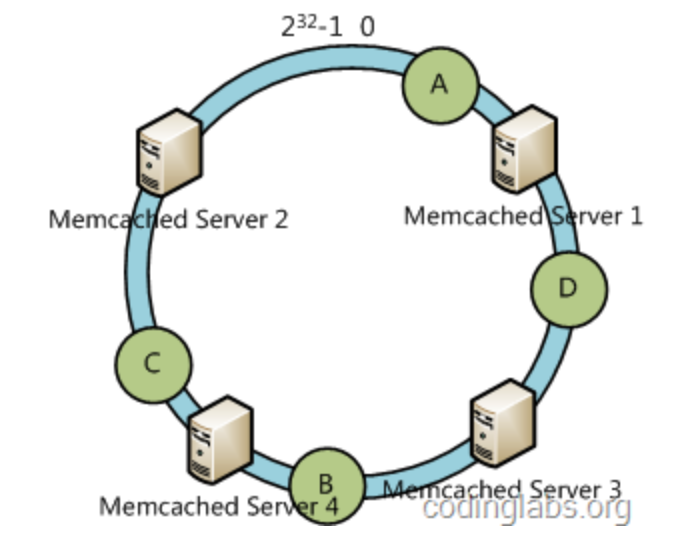
\includegraphics[width=0.3\textwidth]{system-hashing-ring-5}
\caption{增加Server4}
\label{fig:system-hashing-ring-5}
\end{figure}

此时 A、D、C 不受影响,只有 B 需要重定位到新的 Server 4。一般的,在一致性哈希算法中,如果增加一台服务器,则受影响的数据
仅仅是新服务器到其环空间中前一台服务器(即顺着逆时针方向行走遇到的第一台服务器)之间数据,其它不会受到影响。

综上所述,一致性哈希算法对于节点的增减都只需重定位环空间中的一小部分数据,具有较好的容错性和可扩展性。

\noindent\textbf{虚拟节点}

一致性哈希算法在服务节点太少时,容易因为节点分部不均匀而造成数据倾斜问题。例如我们的系统中有两台服务器,其环分布如图%
\ref{fig:system-hashing-ring-6}:

\begin{figure}[hbtp]
\centering
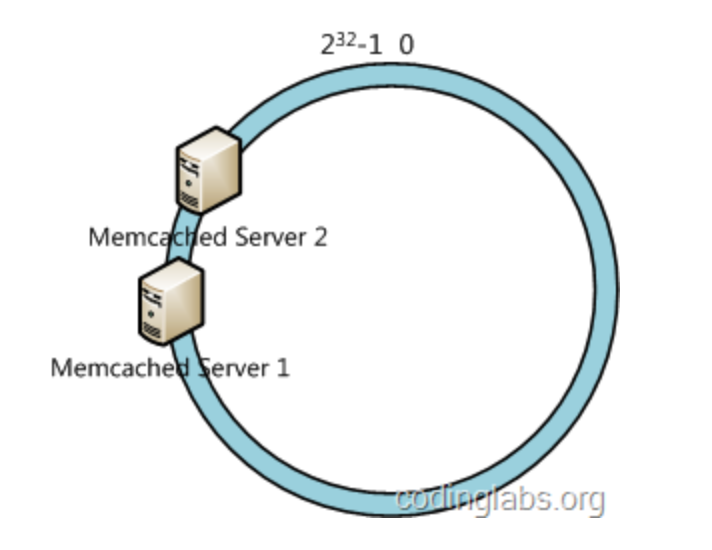
\includegraphics[width=0.3\textwidth]{system-hashing-ring-6}
\caption{节点太少造成的数据倾斜}
\label{fig:system-hashing-ring-6}
\end{figure}

此时必然造成大量数据集中到 Server 1 上,而只有极少量会定位到 Server 2 上。为了解决这种数据倾斜问题,一致性哈希算法引入了
虚拟节点机制,即对每一个服务节点计算多个哈希,每个计算结果位置都放置一个此服务节点,称为虚拟节点。具体做法可以在服务器 ip 或主机名
的后面增加编号来实现。例如上面的情况,我们决定为每台服务器计算三个虚拟节点,于是可以分别计算 “Memcached Server 1\#1”、
“Memcached Server 1\#2”、“Memcached Server 1\#3”、“Memcached Server 2\#1”、“Memcached Server 2\#2”、
“Memcached Server 2\#3” 的哈希值,于是形成六个虚拟节点:

\begin{figure}[hbtp]
\centering
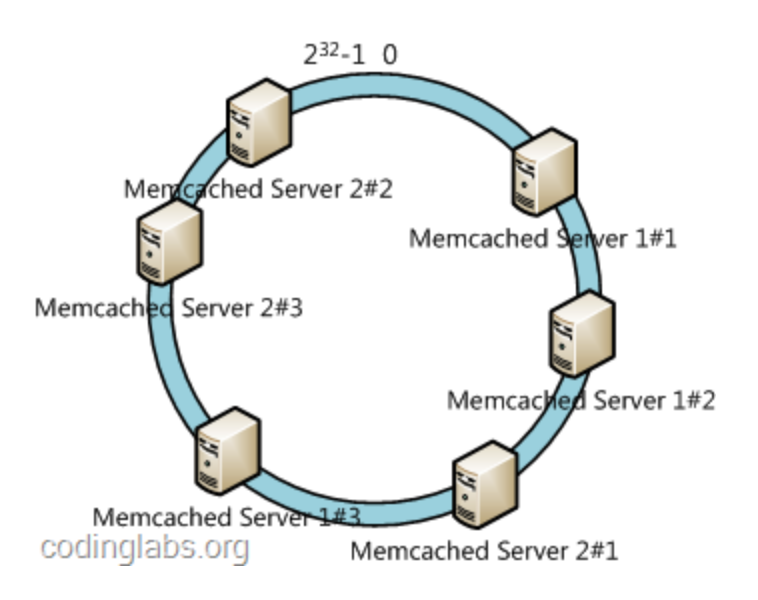
\includegraphics[width=0.3\textwidth]{system-hashing-ring-7}
\caption{使用虚拟节点来实现负载均衡}
\label{fig:system-hashing-ring-7}
\end{figure}

同时数据定位算法不变,只是多了一步虚拟节点到实际节点的映射,例如定位到 “Memcached Server 1\#1”、“Memcached Server 1\#2”、
“Memcached Server 1\#3” 三个虚拟节点的数据均定位到 Server 1 上。这样就解决了服务节点少时数据倾斜的问题。
在实际应用中,通常将虚拟节点数设置为 32 甚至更大,因此即使很少的服务节点也能做到相对均匀的数据分布。

\noindent\textbf{总结}

目前一致性哈希基本成为了分布式系统组件的标准配置,例如 Memcached 的各种客户端都提供内置的一致性哈希支持。本节只是简要介绍了这个算法,
更深入的内容可以参看原论文。














\endinput

\chapter{机器学习 \& 深度学习基础}\label{chap:deeplearning}
\addtocontents{los}{\protect\addvspace{10pt}}

\begin{intro}

\end{intro}

\section{梯度下降}\label{sec:gradient-descent}

\subsection{损失函数}\label{loss-function}

\subsection{过拟合}\label{overfit}

\subsection{正则化}\label{regularized}


\section{Inference \& Training}\label{sec:inference-training}

\subsection{}\label{}


\endinput
\chapter{RDMA 相关知识点整理}\label{chap:rdma}
\addtocontents{los}{\protect\addvspace{10pt}}

\begin{intro}

\end{intro}

\section{}

\subsection{}

\subsection{}


\endinput
\chapter{算法与数据结构}\label{chap:algorithms}
\addtocontents{los}{\protect\addvspace{10pt}}

\begin{intro}

\end{intro}

\section{基本数据结构}\label{sec:primary-data-structures}

\begin{itemize}
\item 算法第四版 C++ 实现
\item 浅谈算法和数据结构%
  \footnote{https://www.cnblogs.com/yangecnu/category/548373.html}%
\end{itemize}

\section{分而治之}\label{sec:divide-and-conquer}


\section{贪心}\label{sec:greedy}

\subsection{}

\subsection{}


\section{动态规划}\label{sec:dynamic-programming}

\begin{quotation}
以下内容整理自:

\begin{itemize}
  \item 知乎上问题『什么是动态规划?动态规划的意义是什么?』
  \item 算法导论 Chapter 15 % TODO
  \item 算法 Chapter 6 % TODO 
\end{itemize}
\end{quotation}

\subsection{动态规划的本质}

动态规划的本质,是对问题\textbf{状态的定义}和\textbf{状态转移方程的定义}。引用维基百科:
\begin{quotation}
\textbf{Dynamic programming} is a method for solving a complex problem by \textbf{breaking it down
into a collection of simpler subproblems.}
\end{quotation}
动态规划就是通过\textbf{拆分问题},定义问题状态和状态之间的关系,使得问题能够以递推(或者说分治)的方式去解决。
\textbf{如何拆分问题},才是动态规划的核心。而\textbf{拆分问题},靠的就是\textbf{状态的定义}和\textbf{状态转移方程的定义}。

\subsection{状态的定义}

首先来看一个动态规划的教学必备题:
\begin{quotation}
给定一个数列,长度为$N$,求这个数列的最长上升(递增)子序列(LIS)的长度。以 1\quad7\quad2\quad8\quad3\quad4 为例,这个数列的
最长递增子序列是 1\quad2\quad3\quad4,长度为 4;次长的为 3,包括 1\quad7\quad8、1\quad2\quad3、1\quad3\quad4。
\end{quotation}
要解决这个问题,首先要\textbf{定义这个问题}和\textbf{这个问题的子问题}。
有人可能会问了,题目都已经在这了,还需定义这个问题吗?需要,原因就是这个问题在字面上看,找不出子问题,而没有子问题,这个题目就
没办法解决。

所以,重新定义这个问题:
\begin{quotation}
给定一个数列,长度为$N$,设 $F_{k}$ 为:以数列中第 $k$ 项结尾的最长递增子序列的长度。求 $F_{1}, \cdots, F_{N}$ 中的最大值。
\end{quotation}
显然,这个新问题与原问题等价。而对于 $F_{k}$ 来讲,$F_{1}, \cdots, F_{k-1}$ 都是 $F_{k}$ 的子问题:因为以第 $k$ 项结尾的
最长递增子序列(以下称 LIS),包含着以第 $1, \cdots, k-1$ 中某项结尾的 LIS。

上述的新问题 $F_{k}$ 也可以叫做状态,定义中的『$F_{k}$ 为数列中第 $k$ 项结尾的 LIS 的长度』,就叫做对状态的定义。之所以把 $F_{k}$
叫做『状态』而不是『问题』,一是因为避免跟原原题中的『问题』混淆,二是因为这个新问题是数学化定义的。

对状态的定义只有一种吗?当然不是。我们甚至可以二维的,以完全不同的视角定义这个问题:
\begin{quotation}
给定一个数列,长度为$N$,设 $F_{i, k}$ 为:在前 $i$ 项中的长度为 $k$ 的最长递增子序列中,最后一位的最小值。其中 $1 \leq k \leq N$ 。
若在前 $i$ 项中,不存在长度为 $k$ 的最长递增子序列,则 $F_{i, k}$ 为正无穷。求最大的 $x$,使得 $F_{N, x}$ 不为正无穷。
\end{quotation}
上述的 $F_{i, k}$ 就是状态,定义中的『$F_{i, k}$ 为:在前 $i$ 项中的长度为 $k$ 的最长递增子序列中,最后一位的最小值』就是对
状态的定义。

\subsection{状态转移方程}

上述状态定义好之后,状态和状态之间的关系式,就叫做\textbf{状态转移方程}。

比如,对于 LIS 问题,第一种定义:
\begin{quotation}
设 $F_{k}$ 为:以数列中第 $k$ 项结尾的最长递增子序列的长度。
\end{quotation}
设 $A$ 为题中数列,状态转移方程为:
\begin{quotation}
$F_{1} = 1$(根据状态定义导出边界情况)

$F_{k} = max(F_{i} + 1 | A_{k} > A_{i}, i \epsilon (1\cdots k-1)) (k > 1)$
\end{quotation}
用文字解释一下是:以第 $k$ 项结尾的 LIS 的长度是,保证第 $i$ 项比第 $k$ 项小的情况下,以第 $i$ 项结尾的 LIS 长度加一的最大值,取遍 $i$
的所有值($i < k$)。

第二种定义:
\begin{quotation}
设 $F_{i, k}$ 为:在前 $i$ 项中的长度为 $k$ 的最长递增子序列中,最后一位的最小值。
\end{quotation}
设 $A$ 为题中数列,状态转移方程为:
\begin{quotation}
若 $A_{i} > F_{i-1, k-1}$,$F_{i, k} = min(A_{i}, F_{i-1, k})$;否则 $F_{i, k} = F_{i-1, k}$。
\end{quotation}
这里可以看出,状态转移方程,就是定义了问题和子问题之间的关系。可以看出,状态转移方程就是带有条件的递推式。

\subsection{动态规划迷思}

\noindent\textbf{缓存,重叠子问题,记忆化}

这三个名词,都是在阐述递推式求解的技巧。以 Fibonacci 数列为例,计算第 100 项的时候,需要计算第 99 项和第 98 项;在计算第 101 项的时候,需要第
100 项和第 99 项。这时候你还需要重新计算第 99 项吗?不需要,你只需要在第一次计算的时候把它记下来就可以了。上述的需要再次计算的『第 99 项』,就叫
『重叠子问题』。如果没有计算过,就按照递推式计算,如果计算过,直接使用,就像『缓存』一样,这种方法,叫做『记忆化』,这是递推式求解的技巧。这种技巧,
通俗的说叫『花费空间来节省时间』。\textbf{都不是动态规划的本质,不是动态规划的核心。}

\noindent\textbf{递归}

递归是递归是求解的方法,连技巧都算不上。

\noindent\textbf{无后效性,最优子结构}

上述的状态转移方程中,等式右边不会用到下标大于左边 $i$ 或者 $k$ 的值,这是『无后效性』的通俗上的数学定义,符合这种定义的状态定义,我们可以说她他具有
『最有子结构』的性质,在动态规划中我们要做的,就是找到这种『最优子结构』。

在对状态和状态转移方程的定义过程中,满足『最优子结构』是一个隐含条件(否则根本定义不出来)。对状态和和『最优子结构』的进一步理解\textbf{TODO}

\begin{newnote}[对状态和和『最优子结构』的进一步理解]
动态规划是对于\textbf{某一类问题}的解决方法!重点在于如何鉴定『某一类问题』是动态规划可解的,而不是纠结解决方法是递归还是递推!

怎么鉴定动态规划可解的一类问题,需要从计算机是怎么工作的说起。计算机的本质是一个状态机,内存里存储的所有数据构成了当前的状态,CPU 只能利用当前的状态
计算出下一个状态(不要纠结硬盘之类的外部存储,就算考虑它们也只是扩大了状态的存储容量而已,并不能改变下一个状态只能从当前状态计算出来这一条铁律)。
当你企图使用计算机解决一个问题是,其实就是在思考如何将这个问题表达成状态(用哪些变量存储哪些数据)以及如何在状态中转移(怎样根据一些变量计算出
另一些变量)。所以,所谓的空间复杂度就是为了支持你的计算所必需存储的状态最多有多少,所谓时间复杂度就是从初始状态到达最终状态中间需要多少步!
\end{newnote}

一个问题是该用递推、贪心、搜索还是动态规划,完全是由这个问题本身阶段间状态的转移方式决定的!
\begin{itemize}
	\item 每个阶段只有一个状态 $\rightarrow$ 递推;
	\item 每个阶段的最优状态都是由上一个阶段的最优状态得到的 $\rightarrow$ 贪心;
	\item 每个阶段的最优状态是由之前所有阶段的状态的组合得到的 $\rightarrow$ 搜索;
	\item 每个阶段的最优状态可以从之前某个阶段的某个或某些状态直接得到而不管之前这个状态是如何得到的 $\rightarrow$ 动态规划。
\end{itemize}

『每个阶段的最优状态可以从之前某个阶段的某个或某些状态直接得到』,这个性质叫做\textbf{最优子结构};而不管之前这个状态是如何得到的,这个性质
叫做\textbf{无后效性}。

需要注意的是,一个问题可能有多种不同的状态定义和状态转移方程定义,存在一个有后效性的定义,不代表该问题不适合动态规划。动态规划方法要寻找符合『最优子结构』
的状态和状态转移方程的定义,在找到之后,这个问题就亦可以以『记忆化地求解递推式』的方法来解决。而寻找到的定义,才是动态规划的本质。即,\textbf{动态规划
是寻找一个对问题的观察角度,让问题能够以递推(或者说分治)的方式去解决,寻找看问
题的角度,才是动态规划中最耀眼的宝石!}


\section{回溯法}\label{sec:back-tracking}



\section{分支限界法}\label{sec:branch-and-bound}




\endinput

\chapter{秋招准备}\label{chap:interviews}
\addtocontents{los}{\protect\addvspace{10pt}}

\begin{intro}
整理各面经上的经典面试题,将各个思路进行一个系统化的梳理。
\end{intro}

\section{算法题}

\subsection{判断是否有环?}

\begin{quotation}
{\color{red}如何判断一个链表是否有环?}
\end{quotation}

\begin{enumerate}
\item 最简单也是最直接的想法,从头遍历链表,将已经遍历过的节点信息保存起来,可以
  在遍历一个新节点时,查看该节点之前是否已经遍历过了,增加一个 tag 标记;或者将
  已经遍历过的节点信息使用 HashMap 保存起来,当遍历到一个新节点时,直接查表看之
  前是否已经遍历过该节点。
\item 使用两个指针 slow 和 fast,在刚开始时这两个指针均指向链表首节点,slow 每
  次向前走一步(slow = slow->next;),fast 每次向前走两步
  (fast = fast->next->next;),需要我们自己去判断是否 next 合法,比较 slow
  和 fast 指针指向的节点,如果相同,说明该链表有环;如果不同,继续进行下一次循环
  (slow 向前走一步,fast 向前走两步)。当链表中确实存在环的时候,slow 和 fast
  最终会指向同一个节点;若不存在环,可以通过 fast 达到链表结尾处来结束算法循环。
\end{enumerate}

环形链表的问题可以引申出更多的算法问题,比如:

\begin{enumerate}
  \item [问题一] 在一个有环链表中,如何知道环的长度?如何找出链表的入环点?
  \begin{itemize}
  \item slow 和 fast 第一次相遇可以用于判断链表是否有环,记录下该碰撞点 p,
    slow 和 fast 再次于节点 p 相遇即为环的长度。
  \item 碰撞点 p 到入环点的距离等于头节点到入环点的距离,因此,当 slow 和 fast
    第一次相遇得到碰撞点 p 之后,从碰撞点 p 和头节点开始走(每次走一步),相遇的
    那个点就是入环点。
  \end{itemize}
  \item [问题二] 判断两个单向链表是否相交,如果相交,求出交点。
  \item [问题三] 用于找到链表的中间元素。使用快慢指针(slow 和 fast)可以实现。
\end{enumerate}


\noindent\rule[0.25\baselineskip]{\textwidth}{1pt}

\begin{quotation}
{\color{red}一个有向图用邻接矩阵表示,并且是有权图,现在怎么判断图中有没有环?}
\end{quotation}

拓扑排序的思想可以借鉴。



\subsection{排序算法}\label{subsec:sort-algorithms}


\begin{quotation}
  {\color{red}各种排序算法总结}%
  \footnote{http://www.cnblogs.com/wxisme/p/5243631.html}%
\end{quotation}


\noindent\rule[0.25\baselineskip]{\textwidth}{1pt}

\begin{quotation}
{\color{red}实现快速排序?}
\end{quotation}

\textbf{TODO} 待整理


\noindent\rule[0.25\baselineskip]{\textwidth}{1pt}

\begin{quotation}
  {\color{red}被忽视的 partition 算法}%
  \footnote{https://selfboot.cn/2016/09/01/lost\_partition/}%
\end{quotation}



\subsection{二分查找}\label{subsec:binary-search}

\begin{quotation}
  {\color{red}实现最简单的二分查找,分析二分查找代码实现中需要注意的地方,另外整理可以使用二
  分查找思想来做的一系列题目。}
\end{quotation}


\section{C / C++}\label{sec:c-and-cplusplus}

\subsection{基础知识}

\begin{quotation}
  {\color{red}sizeof 运算符}
\end{quotation}

\verb|sizeof| 运算符返回一条表达式或一个类型名字所占的字节数。 \verb|sizeof| 运
算符满足右结合律,其所得的值是一个 \verb|size_t| 类型的常量表达式(在编译时即可
确定值)。 \verb|sizeof| 运算符的运算对象有两种形式:

\qquad \verb|sizeof (type)| \quad or \quad \verb|sizeof expr|

在第二种形式中, \verb|sizeof| 返回的是表达式结果类型的大小。与众不同的一点是,
\verb|sizeof| 并不实际计算其运算对象的值。

\verb|sizeof| 运算符的结果部分地依赖于其作用的类型:
\begin{itemize}
\item 对 \verb|char| 或者类型为 \verb|char| 的表达式执行 \verb|sizeof| 运算,结
  果得 1;
\item 对引用类型执行 \verb|sizeof| 运算符得到被引用对象所占空间的大小;
\item 对指针执行 \verb|sizeof| 运算得到指针本身所占空间的大小;
\item 对解引用指针执行 \verb|sizeof| 运算得到指针指向的对象所占空间的大小,指针
  不需有效;
\item 对数组执行 \verb|sizeof| 运算得到整个数组所占空间的大小。注意,
  \verb|sizeof| 运算不会把数组转换成指针来处理;
\item 对 \verb|string| 对象或 \verb|vector| 对象执行 \verb|sizeof| 运算只返回该
  类型固定部分的大小,不会计算对象中的元素占用了多少空间。
\end{itemize}


\noindent\rule[0.25\baselineskip]{\textwidth}{1pt}

\begin{quotation}
  {\color{red}C 的结构体和 C++ 结构体的区别}
\end{quotation}

\begin{itemize}
\item C 的结构体内不允许有函数存在,C++ 允许有内部成员函数,且允许该函数是虚函数。
  所以 C 的结构体是没有构造函数、析构函数、和 \verb|this| 指针的。
\item C 的结构体对内部成员变量的访问权限只能是 public,而 C++ 允许
  \verb|public| 、 \verb|protected| 、 \verb|private| 三种。
\item C 语言的结构体是不可以继承的,C++ 的结构体是可以从其他的结构体或者类继承过
  来的。
\end{itemize}

以上都是表面的区别,实际区别就是面向过程和面向对象编程思路的区别:

C 的结构体只是把数据变量给包裹起来了,并不涉及算法。而 C++ 是把数据变量及对这些
数据变量的相关算法给封装起来,并且给对这些数据和类不同的访问权限。C 语言中是没有
类的概念的,但是 C 语言可以通过结构体内创建函数指针实现面向对象思想。


\noindent\rule[0.25\baselineskip]{\textwidth}{1pt}

\begin{quotation}
  {\color{red}C++ struct 和 class 关键字}
\end{quotation}

\begin{itemize}
\item \verb|struct| 和 \verb|class| 都可以用来定义一个类;
\item \verb|struct| 和 \verb|class| 的默认访问权限不太一样;
\item 类可以在它的第一个访问说明符之前定义成员,对这种成员的访问权限依赖于类定义
  的方式。如果使用 \verb|struct| 关键字,则定义再第一个访问说明符之前的成员是
  \verb|public| 的;相反,如果使用 \verb|class| 关键字,则这些成员是
  \verb|private| 的。
\end{itemize}


\noindent\rule[0.25\baselineskip]{\textwidth}{1pt}

\begin{quotation}
  {\color{red}C++ 引用和指针}
\end{quotation}



\noindent\rule[0.25\baselineskip]{\textwidth}{1pt}

\begin{quotation}
  {\color{red}C 语言中的字符串}
\end{quotation}

\noindent 整理自 \textbf{C 程序设计语言(第2版)} 5.5 字符指针与函数,中文版页码 89

字符串常量 是一个字符数组,例如:

\verb|``hello, world\n'';|

\noindent 在字符串的内部表示中,字符数组以空字符 \verb|`\0'| 结尾,程序可以通过检查空字符
找到字符数组的结尾。字符串常量占据的存储单元数也因此比双引号内的字符数大 1。

字符串常量最常用的用法也许是作为函数参数,例如:

\verb|printf(``hello, world.\n'');|

\noindent 当类似于这样的一个字符串出现在程序中时,实际上是通过字符指针访问该字符串的。在上
述语句中, \verb|printf| 接受的是一个指向字符数组第一个字符的指针。也就是说,字符串常量
可通过一个指向其第一个元素的指针来访问。

除了作为函数参数外,字符串常量还有其他用法。假定指针 \verb|pmessage| 的声明如下:

\verb|char *pmessage;|

\noindent 那么,语句

\verb|pmessage = ``hello, world\n'';|

\noindent 将把一个指向该字符数组的指针赋值给 \verb|pmessage| 。该过程并没有进行字符串的复制,而只
是涉及到指针的操作。C 语言没有提供将整个字符串作为一个整体进行处理的运算符。下
面两个定义之间有很大的差别:

\verb|char amessage[] = ``hello, world\n'';  // 定义了一个数组|

\verb|char *pmessage = ``hello, world\n'';  // 定义了一个指针|

上述声明中, \verb|amessage| 是一个仅仅保存足以存放初始化字符串以及空字符
\verb|`\0'| 的一维数组。数组中的单个字符可以进行修改,但 \verb|amessage| 始终指向同一存
储位置。另一方面, \verb|pmessage| 是一个指针,其初值指向一个字符串常量,之后它可以被
修改以指向其他地址,但如果试图通过 \verb|pmessage| 指针修改字符串的内容,结果是没
有定义的(会出现段错误 \verb|Segment Fault| )。

另外,在页码 85 中有描述:

在函数定义中,形式参数 \verb|char s[]| 和 \verb|char *s| 是等价的。我们通常更习
惯于使用后一种形式,因为它比前者更直观地表明了这个参数是一个指针。如果将数组名传
递给函数,函数可以根据情况判定是按照数组处理还是按照指针处理,随后根据相应的方式
操作该参数。为了直观且恰当地描述函数,在函数中甚至可以同时使用数组和指针这两种表
示方法。

另外我们可以从汇编的角度来理解:

第一个字符串是用数组开辟的,它是可以改变的变量。

\begin{sourcecode}[hbtp]
\begin{Verbatim}
movq    L_main.amessage(%rip), %rax
movq    %rax, -22(%rbp)
movl    L_main.amessage+8(%rip), %ecx
movl    %ecx, -14(%rbp)
movw    L_main.amessage+12(%rip), %dx
movw    %dx, -10(%rbp)
movb    \$72, -22(%rbp)  %% TODO
\end{Verbatim}
\caption{amessage 数组表示的汇编代码}
\end{sourcecode}

而第二个字符串则是一个常量,也就是字面值。 \verb|pmessage| 只是指向它的指针而已,
而不能改变指向的内容。

\begin{sourcecode}[hbtp]
\begin{Verbatim}
leaq    L_.str(%rip), %rcx
\end{Verbatim}
\caption{pmessage 指针表示的汇编代码}
\end{sourcecode}

可见用数组和用指针是完全不相同的。

要想通过指针来改变常量是错误,正确的写法应该是用 \verb|const| 指针。

\verb|const char *pmessage = ``hello, world\n'';|

\noindent\rule[0.25\baselineskip]{\textwidth}{1pt}

\begin{quotation}
  {\color{red} C++ 中 string 的使用小结}
\end{quotation}

正是因为 C 风格字符串(以空字符结尾的字符数组)太过复杂难于掌握,不适合大程序的开
发,所以 C++ 标准库定义了一种 \verb|string| 类,定义在头文件 \verb|<string>|。

可以使用 C 风格字符串来初始化 C++ 中的 \verb|string| 对象实例,

\verb|string str(``hello, world\n'');  // correct|

\noindent 但是如果直接将 \verb|string| 类型的对象赋值给 C 风格的字符串的话,编译器会报错,

\verb|char *pstr = str;  // error|

\noindent 但是实际应用中这个问题也难以避免,很多时候还是需要将 \verb|string| 类型的转化为
\verb|char*| 来实现自定义的操作,C++ 标准库也为了和之前用 C 写的程序兼容,于是可
以用 \verb|string| 的 \verb|c_str()| 函数。

\verb|char *pstr = str.c_str();  // error|

\noindent\verb|c_str()| 为了防止意外地修改 \verb|string| 对象,返回的是 \verb|const|
指针,所以上面这段代码是不能被编译的。正确的应该是用 \verb|const| 指针。

\verb|const char *pstr = str.c_str();  // correct|

这个 \verb|c_str()| 方法在 C++ IO 流操作上也被广泛应用。在打开文件时,如果要指定
文件名,可以用 C 风格的字符串。如果用到 \verb|string| 类型的字符串作为文件名时,
就必须调用 \verb|c_str()| 方法将其转换为一个 C 风格字符串。

\begin{sourcecode}[hbtp]
\begin{Verbatim}
string   filename;  //定义文件名称
cin >> filename;
ifstream.open(filename.c_str());  //要使用 C 风格字符串
\end{Verbatim}
\caption{c\_str() 在 C++ IO 流操作上的应用}
\end{sourcecode}

对 \verb|string| 有一定了解后,C++ 标准库还定义的一系列丰富的字符串操作,均基于
\verb|string| 类型。从某一种程度上来说, \verb|string| 就是一种字符容器。

标准库为 \verb|string| 定义了很多方法,包括构造、插入( \verb|insert| )、替换(
\verb|assign| 和 \verb|replace| )、比较( \verb|compare| )、查找( \verb|find| )、
删除( \verb|erase| )、连接( \verb|append| )以及对子串的操作( \verb|substr| ),并
且每一类操作都有很多种重载。%
\footnote{http://www.cnblogs.com/gaojun/archive/2010/09/11/1824016.html}%

\noindent\rule[0.25\baselineskip]{\textwidth}{1pt}

\begin{quotation}
  {\color{red}\verb|std::endl| 与 \verb|`\n'| 有什么区别?在执行的功能上?}
\end{quotation}

\verb|std::endl| 是一个被称为\textbf{操纵符}(manipulator)的特殊值。写入 \verb|std::endl| 的效果是结束
当前行,并将与设备相关联的缓冲区(buffer)中的内容刷到设备中。缓冲刷新操作可以保
证到目前为止程序所产生的所有输出都真正写入输出流,而不是仅停留在内存中等待写入流。

在调试程序时,通常会添加打印语句。这类语句应该保证『一直』刷新流,否则,如果程序
崩溃,输出可能还留在缓冲区中,从而导致关于程序崩溃位置的错误推断。

\verb|`\n'| 为 C++ 语言规定的转义序列之一,\textbf{换行符}

\begin{newnote}[StackExchange 上一个 CodeReview 上的解释]
  The main difference in the two is that std::endl in addition to adding $\backslash$n to
  the stream will flush the stream. The stream will already auto flush at the
  optimal times and forcing a manual flush will only result in a degradation in
  performance.
\end{newnote}

\noindent 何时适用 \verb|std::endl| ,何时适用 \verb|`\n'| 呢?

由于流操作符 \verb|operator<<| 的重载,对于 \verb|`\n'| 和 \verb|``\n''| ,输出效果相同。

对于有输出缓冲的流(例如 \verb|std::cout| 、 \verb|std::clog| ),如果不手动进行缓冲区刷新操作,将在缓冲区
满后自动刷新输出。不过对于 \verb|std::cout| 来说(相对于文件输出流等),缓冲一般体现得并不明
显。但是必要情况下使用 \verb|std::endl| 代替 \verb|`\n'| 一般是个好习惯。

对于无缓冲的流(例如标准错误输出流 \verb|std::cerr| ),刷新是不必要的,可以直接
使用 \verb|`\n'| ,过多的 \verb|std::endl| 是影响程序执行效率低下的因素之一。

由于直接输入/输出和操作系统相关,可能需要切换内核态/用户态,需要一定的时间开销,
频繁地进行操作会极大地降低输入/输出的效率,所以标准库对流的输入/输出操作使用缓冲。
具体来讲,就是在内存中保存一个大小相对固定的区域(缓冲区)用来储存临时的输入或输
出。当必要时,才向系统设备复制缓冲区的内容并清空缓冲区,这个过程称为刷新。

\verb|std::cout << std::endl;|

is equivalent to

\verb|std::cout << `\n' << std::flush;|

So,
\begin{itemize}
\item Use \verb|std::endl| if you want to force an immediate flush to the output.
\item Use \verb|`\n'| if you are worried about performance (which is probably not the
  case if you are using the \verb|<<| operator).
\end{itemize}


\noindent\rule[0.25\baselineskip]{\textwidth}{1pt}

\begin{quotation}
  {\color{red}C++ 中的声明与定义的关系}
\end{quotation}

TODO


\noindent\rule[0.25\baselineskip]{\textwidth}{1pt}

\begin{quotation}
  {\color{red}C++ 中的四个关键字: const / extern / static / volatile }
\end{quotation}

\noindent\textbf{const}

\begin{itemize}
\item 修饰基本数据类型和类类型,说明其为常量,不能修改
\item 修饰指针 \textbf{从右向左进行定义的理解}
  \begin{itemize}
  \item [-] 指向常量的指针(pointer to const) \verb|const| 在 \verb|*| 左边,指
    针指向的是常量,不能使用此指针来改变其所指对象的值
  \item [-] 常量指针(const pointer) \verb|const| 在 \verb|*| 右边,指针本身为
    常量,即不变的是指针本身的值而非指向的那个值。常量指针必须初始化,而且一旦初
    始化完成,则它的值(也就是存放在指针中的那个地址)就不能再改变了
  \end{itemize}
\item 修饰函数参数和返回值,与上一 item 中的『修饰指针』描述相同
\item 修饰类中的数据成员,
\item 修饰类中的成员函数

  \begin{sourcecode}[hbtp]
    \begin{Verbatim}
      struct Sales_data {
        std::string isbn() const { return bookNo; }

        std::string bookNo;
      };
    \end{Verbatim}
    \caption{C++ Primer 上 Sales\_data 类的例子}
  \end{sourcecode}

  类中的成员函数在被调用时,成员函数通过一个名为 \verb|this| 的额外隐式函数来访
  问调用它的那个对象。当我们调用一个成员函数时,用请求该函数的对象地址初始化
  \verb|this| 。例如,如果调用 \verb|total.isbn();| ,则编译器负责把
  \verb|total| 的地址传递给 \verb|isbn| 的隐式形参 \verb|this| ,可以等价地认为
  编译器将该调用重写成了 \verb|Sales_data::isbn(&total);| ,其中,调用
  \verb|Sales_data| 的 \verb|isbn| 成员时传入了 \verb|total| 的地址。

  在成员函数内部,我们可以直接使用调用该函数的对象的成员,而无需通过成员访问运算
  符来做到这一点,因为 \verb|this| 所指的正是这个对象。任何对类成员的直接访问都
  被看作 \verb|this| 的隐式引用,也就是说,当 \verb|isbn| 使用 \verb|bookNo| 时,
  它隐式地使用 \verb|this| 指向的成员,就像写为 \verb|this->bookNo| 一样。

  \verb|this| 形参是隐式定义的,我们可以在成员函数体内部使用 \verb|this|

  \begin{sourcecode}[hbtp]
    \begin{Verbatim}
      struct Sales_data {
        std::string isbn() const { return this->bookNo; }

        std::string bookNo;
      };
    \end{Verbatim}
    \caption{C++ Primer 上 Sales\_data 类的例子,添加上 this}
  \end{sourcecode}

  因为 \verb|this| 总是指向『这个』对象,所以 \verb|this| 是一个常量指针,我们不
  允许改变 \verb|this| 中保存的地址。

  默认情况下, \verb|this| 的类型是指向类类型\textbf{非常量版本}的\textbf{常量指针}。例如在上面的
  \verb|Sales_data| 的成员函数中, \verb|this| 的类型是
  \verb|Sales_data *const| 。尽管 \verb|this| 是隐式的,它仍然需要遵循初始化规则,
  意味着(在默认情况下)我们不能把 \verb|this| 绑定到一个常量对象上。这一情况也
  就使得我们不能在一个常量对象上调用普通的成员函数。

  如果 \verb|isbh| 是一个普通函数而且 \verb|this| 是一个普通的指针参数,则我们应
  该把 \verb|this| 声明成

  \qquad \verb|const Sales_data *const|

  毕竟,在 \verb|isbn|
  的函数体内不会改变 \verb|this| 所指的对象,所以把 \verb|this| 设置为指向常量的
  指针有助于提高函数的灵活性。

  然而, \verb|this| 是隐式的并且不会出现在参数列表中,所以在哪里将 \verb|this|
  声明成指向常量的指针就是我们必须面临的问题。C++ 语言的做法是允许把
  \verb|const| 关键字放在成员函数的参数列表之后,此时,紧跟在参数列表后面的
  \verb|const| 表示 \verb|this| 是一个指向常量的指针。称为\textbf{常量成员函数}
  (const member function)。

  \begin{sourcecode}[hbtp]
    \begin{Verbatim}
      // 伪代码,说明隐式的 this 指针是如何使用的
      // 下面的代码是非法的:因为我们不能显式地定义自己的 this 指针
      // 谨记此处地 this 是一个指向常量的指针,因为 isbn 是一个常量成员
      std::string Sales_data::isbn(const Sales_data *const this) {
        return this->bookNo;
      }
    \end{Verbatim}
    \caption{C++ Primer 上 Sales\_data 类的 isbn 成员函数伪代码}
  \end{sourcecode}

  因为 \verb|this| 是一个指向常量的指针,所以常量成员函数不能改变调用它的对象的
  内容。在上面的例子中, \verb|isbn| 可以读取调用它的对象的数据成员,但是不能写
  入新值。
  
\end{itemize}

\noindent\textbf{extern}

\begin{itemize}
\item 引用其他文件中的 \verb|const| 变量

  当以编译时初始化的方式定义一个 \verb|const| 对象时,编译器将在编译过程中把用到
  该变量的地方都替换成对应的值。为了执行此替换,编译器必须知道变量的初始值。如果
  程序包含多个文件,则每个用了 \verb|const| 对象的文件都必须得能访问到它的初始值
  才行。要做到这一点,就必须在每一个用到变量的文件中都有对它的定义。为了支持这一
  用法,同时避免对同一变量的重复定义,默认情况下, \verb|const| 对象被设定为仅在
  文件内有效。当多个文件中出现了同名的 \verb|const| 变量时,其实等同于在不同文件
  中分别定义了独立的变量。

  某些时候有这样一种 \verb|const| 变量,它的初始值不是一个常量表达式,但又确实
  有必要在文件间共享。解决办法是,对于 \verb|const| 变量不管是声明还是定义都添加
  \verb|extern| 关键字,这样只需要定义一次就可以了:

  \begin{sourcecode}[hbtp]
    \begin{Verbatim}
      // example.cc 定义并初始化了一个常量,该常量能被其他文件访问
      extern const int bufSize = fcn();
      // example.h 头文件
      extern const int bufSize;  // 与 example.cc 中定义的 bufSize 是同一个
    \end{Verbatim}
    \caption{在多个文件之间共享 const 对象,必须在变量的定义之前添加 extern}
  \end{sourcecode}

\item C++ 程序有时候需要调用其他语言编写的函数,最常见的是调用 C 语言编写的函数。
  需使用 \verb|extern| 关键字
\end{itemize}

\noindent\textbf{static}

C++ 的 \verb|static| 有两种用法:面向过程程序设计中的 \verb|static| 和面向对象程
序设计中的 \verb|static| 。前者应用于普通变量和函数,不涉及类;后者主要说明
\verb|static| 在类中的作用。

\noindent\textbf{面向过程设计中的 static}
\begin{itemize}
\item [1] \textbf{静态全局变量}

  在全局变量前,加上关键字 \verb|static| ,该变量就被定义成为一个静态全局变量。
  静态全局变量有以下特点:
  \begin{itemize}
  \item 该变量在全局数据区分配内存;
  \item 未经初始化的静态全局变量会被程序自动初始化为 0(自动变量的值是随机的,除
    非它被显式初始化);
  \item 静态全局变量在声明它的整个文件都是可见的,而在文件之外是不可见的
  \end{itemize}

  静态变量都在全局数据区分配内存,包括后面将要提到的静态局部变量。对于一个完整的
  程序,在内存中的分布情况如下图:

  \qquad 代码区

  \qquad 全局数据区

  \qquad 堆区

  \qquad 栈区

  一般程序的由 \verb|new| 产生的动态数据存放在堆区,函数内部的自动变量存放在栈区。
  自动变量一般会随着函数的退出而释放空间,静态数据(即使是函数内部的静态局部变量)
  也存放在全局数据区。全局数据区的数据并不会因为函数的退出而释放空间。定义全局变
  量就可以实现变量在文件中的共享,但定义静态全局变量还有几个好处:1)静态全局变
  量不能被其它文件所用;2)其它文件中可以定义相同名字的变量,不会发生冲突。
  
\item [2] \textbf{静态局部变量}

  在局部变量前,加上关键字 \verb|static| ,该变量就被定义成为一个静态局部变量。
  通常,在函数体内定义了一个变量,每当程序运行到该语句时都会给该局部变量分配栈内
  存。但随着程序退出函数体,系统就会收回栈内存,局部变量也相应失效。但有时候我们
  需要在两次调用之间对变量的值进行保存。通常的想法是定义一个全局变量来实现。但这
  样一来,变量已经不再属于函数本身了,不再仅受函数的控制,给程序的维护带来不便。
  静态局部变量正好可以解决这个问题。静态局部变量保存在全局数据区,而不是保存在栈
  中,每次的值保持到下一次调用,直到下次赋新值。

  静态局部变量有以下特点:
  \begin{itemize}
  \item 该变量在全局数据区分配内存;
  \item 静态局部变量在程序执行到该对象的声明处时被首次初始化,即以后的函数调用不
    再进行初始化;
  \item 静态局部变量一般在声明处初始化,如果没有显式初始化,会被程序自动初始化为
    0;
  \item 它始终驻留在全局数据区,直到程序运行结束。但其作用域为局部作用域,当定义
    它的函数或语句块结束时,其作用域随之结束
  \end{itemize}
  
\item [3] \textbf{静态函数}

  在函数的返回类型前加上static关键字,函数即被定义为静态函数。静态函数与普通函数
  不同,它只能在声明它的文件当中可见,不能被其它文件使用。定义静态函数的好处:1)
  静态函数不能被其它文件所用;2)其它文件中可以定义相同名字的函数,不会发生冲突

\end{itemize}

\noindent\textbf{面向对象的 static 关键字(类中的 static 关键字)}
\begin{itemize}
\item [4] \textbf{静态数据成员}

  在类内数据成员的声明前加上关键字 \verb|static| ,该数据成员就是类内的静态数据
  成员。静态数据成员有以下特点:
  \begin{itemize}
  \item 对于非静态数据成员,每个类对象都有自己的拷贝。而静态数据成员被当作是类的
    成员。无论这个类的对象被定义了多少个,静态数据成员在程序中也只有一份拷贝,由
    该类型的所有对象共享访问。也就是说,静态数据成员是该类的所有对象所共有的。对
    该类的多个对象来说,静态数据成员只分配一次内存,供所有对象共用。所以,静态数
    据成员的值对每个对象都是一样的,它的值可以更新;
  \item 静态数据成员存储在全局数据区。静态数据成员定义时要分配空间,所以不能在类
    声明中定义。
  \item 静态数据成员和普通数据成员一样遵从 \verb|public| ,\verb|protected| ,
    \verb|private| 访问规则;
  \item 因为静态数据成员在全局数据区分配内存,属于本类的所有对象共享,所以,它不
    属于特定的类对象,在没有产生类对象时其作用域就可见,即在没有产生类的实例时,
    我们就可以操作它;
  \item 静态数据成员初始化与一般数据成员初始化不同。静态数据成员初始化的格式为:

    \qquad <数据类型><类名>::<静态数据成员名> = <值>
    
  \item 类的静态数据成员有两种访问形式:

    \qquad <类对象名>.<静态数据成员名> or <类类型名>::<静态数据成员名>

    如果静态数据成员的访问权限允许的话(即 \verb|public| 的成员),可在程序中,
    按上述格式来引用静态数据成员;
    
  \item 静态数据成员主要用在各个对象都有相同的某项属性的时候。比如对于一个存款
    类,每个实例的利息都是相同的。所以,应该把利息设为存款类的静态数据成员。这
    有两个好处,1)不管定义多少个存款类对象,利息数据成员都共享分配在全局数
    据区的内存,所以节省存储空间;2)一旦利息需要改变时,只要改变一次,则所
    有存款类对象的利息全改变过来了;
  \item 同全局变量相比,使用静态数据成员有两个优势:1)静态数据成员没有进入程
    序的全局名字空间,因此不存在与程序中其它全局名字冲突的可能性;2)可以实现
    信息隐藏。静态数据成员可以是 \verb|private| 成员,而全局变量不能
  \end{itemize}
  
\item [5] \textbf{静态成员函数}

  与静态数据成员一样,我们也可以创建一个静态成员函数,它是为类类型提供服务而不是
  为某一个类的具体对象服务。静态成员函数与静态数据成员一样,都是类的内部实现,属
  于类定义的一部分。普通的成员函数一般都隐含了一个 \verb|this| 指针,
  \verb|this| 指针指向类的对象本身,因为普通成员函数总是具体的属于某个类的具体对
  象的。通常情况下, \verb|this| 是缺省的。但是与普通函数相比,静态成员函数由于
  不是与任何的对象相联系,因此它不具有 \verb|this| 指针。从这个意义上讲,它无法
  访问属于类对象的非静态数据成员,也无法访问非静态成员函数,它只能访问其余的静态
  成员(包括静态成员变量和静态成员函数)。

  关于静态成员函数,可以总结为以下几点:
  \begin{itemize}
  \item 出现在类体外的函数定义不能指定关键字 \verb|static| ;
  \item 静态成员之间可以相互访问,包括静态成员函数访问静态数据成员和访问静态成员
    函数;
  \item 非静态成员函数可以任意地访问静态成员函数和静态数据成员;
  \item 静态成员函数不能访问非静态成员函数和非静态数据成员;
  \item 由于没有 \verb|this| 指针的额外开销,因此静态成员函数与类的全局函数相比
    速度上会有少许的增长;
  \item 调用静态成员函数,可以用成员访问操作符( \verb|.| )和( \verb|->| )为一个
    类的对象或指向类对象的指针调用静态成员函数,也可以直接使用如下格式:

    \qquad <类名>::<静态成员函数名>(<参数表>)

    调用类的静态成员函数
  \end{itemize}  
\end{itemize}

\verb|static| 关键字总结:
\begin{itemize}
\item 修饰局部变量,把局部变量从栈区移动到静态数据区,改变声明周期,不改变作用域
\item 修饰全局变量,改变作用域,由全工程可见变成本源文件可见
\item 修饰函数,与修饰全局变量相同
\item 修饰类变量,是类的一部分,只有唯一一份副本
\item 修饰类成员函数,没有 \verb|this| 指针,只能访问静态成员(包括静态成员变量
  和静态成员函数)
\end{itemize}

另外可以参看 C++ 中 \verb|static| 作用和使用方法%
\footnote{https://blog.csdn.net/artechtor/article/details/2312766}%


\noindent\textbf{volatile}

\begin{itemize}
\item 谈谈 C/C++ 中的 \verb|volatile| %
  \footnote{https://liam0205.me/2018/01/18/volatile-in-C-and-Cpp/}%
  \quad 在多线程环境下,不应该假设 \verb|volatile| 能够解决多线程中的某些问题,
  而应该选用 C++11 中的互斥量和条件变量,分别在头文件 \verb|mutex| 和
  \verb|condition_varialbe| 。

  \begin{sourcecode}[hbtp]
    \begin{Verbatim}
      // global shared data
      std::mutex m;                   // #include <mutex>
      std::condition_variable cv;     // #include <condition_variable>
      bool flag = false;
      
      thread1() {
        flag = false;
        Type* value = new Type(/* parameters */);
        thread2(value);
        std::unique_lock<std::mutex> lk(m);
        cv.wait(lk, [](){ return flag; });
        apply(value);
        lk.unlock();
        thread2.join();
        if (nullptr != value) { delete value; }
        return;
      }
      
      thread2(Type* value) {
        std::lock_guard<std::mutex> lk(m);
        // do some evaluations
        value->update(/* parameters */);
        flag = true;
        cv.notify_one();
        return;
      }
    \end{Verbatim}
    \caption{使用互斥锁和条件变量实现多线程之间的数据同步,伪代码}
  \end{sourcecode}
  
\item C/C++ 中 \verb|volatile| 关键字详解 %
  \footnote{https://www.cnblogs.com/yc\_sunniwell/archive/2010/07/14/1777432.html}%
\item 易变性:两条语句,如果存在变量重用的话下一条语句会重新从内存中读取;
\item 不可优化:保证含有 \verb|volatile| 的指令一定会被执行,而不会被激进的消除;
\item 顺序性:保证 \verb|volatile| 变量间的顺序性,编译器不会乱序优化,但 CPU 还
  是可能乱序发射执行。
\end{itemize}


\noindent\rule[0.25\baselineskip]{\textwidth}{1pt}

\begin{quotation}
  {\color{red}C++ 中的四种强制类型转换: static\_cast / dynamic\_cast / const\_cast / reinterpret\_cast }
\end{quotation}

一个命名的强制类型转换具有如下形式:

\verb|cast-name<type>(expression);|

\noindent 其中, \verb|type| 是转换的目标类型, \verb|expression| 是要转换的值。
如果 \verb|type| 是引用类型,则结果是左值。 \verb|cast-name| 是 \verb|static_cast| 、
\verb|dynamic_cast| 、 \verb|const_cast| 和 \verb|reinterpret_cast| 中的一种。
\verb|cast-name| 指定了执行的是那种转换。

\noindent\textbf{static\_cast}

\begin{itemize}
\item 允许执行任意的隐式转换和相反的转换动作(无论是否被允许)。也可以用于基础类
  型之间的标准转换;
\item 如类的指针,允许子类类型的指针转换成父类类型的指针(这是一个有效的隐式转
  换),同时,也能够执行相反动作,转换父类为它的子类。
\end{itemize}

\noindent\textbf{dynamic\_cast}

只用于对象的指针和引用。当用与多态类型时,它允许任意的隐式类型转换以及相反过程。
不过,与 \verb|static_cast| 不同,在后一种情况里(注:即隐式转换的相反过程),
\verb|dynamic_cast| 会检查操作是否有效。也就是说,它会检查转换是否会返回一个被
请求的有效的完整对象。 \verb|dynamic_cast| 支持运行时类型识别。 

\noindent\textbf{const\_cast}

操纵传递对象的 \verb|const| 属性,或者是设置或者是移除;一般用于强制消除对象的常
量性。一旦我们去掉了某个对象的 \verb|const| 性质,编译器就不再阻止我们对该对象进
行写操作了。如果对象本身不是一个常量,使用强制类型转换获得写权限是合法的行为。然
而如果对象是一个常量,再使用 \verb|const_cast| 执行写操作就会产生未定义的后果。

只有 \verb|const_cast| 能改变表达式的常量属性,使用其他形式的命名强制类型转换改
变表达式的常量属性都将引发编译器错误。

\noindent\textbf{reinterpret\_cast}

转换一个指针为其他类型的指针,或者转换一个指针为整数类型,操作结果是简单的从一个
指针到别的指针的值得二进制拷贝。

\noindent\textbf{注意:}强制类型转换干扰了正常的类型检查,因此我们强烈建议程序员
避免使用强制类型转换。

\subsection{C++ 语言特性}

\begin{quotation}
  {\color{red}STL}%
  \footnote{STL 源码剖析,侯捷 \quad 著}%
\end{quotation}

\noindent\textbf{各类容器的底层实现}

\begin{center}
  \begin{tabular}{lp{24em}}
    \hline
    容器 & 实现 \\
    \hline
    \textbf{\ttfamily vector} & 数组,支持快速随机访问 \\
    \textbf{\ttfamily deque}  & deque 是一个双端队列(double-ended queue),也是在堆中保存内容的。它的保存形式如下: [heap1] -> [heap2] -> [heap3] 每个堆保存好几个元素,然后堆与堆之间有指针指向,看起来像是 list 和 vector 的结合 \\
    \textbf{\ttfamily list}   & 双向链表,支持快速增删 \\
    \textbf{\ttfamily stack} & 用 list 或 deque 实现,封闭头部 \\
    \textbf{\ttfamily queue} & 用 list 或 deque 实现,封闭头部 \\
    \textbf{\ttfamily priority\_queue} & 底层数据结构一般为 vector 为底层容器,堆 heap 为处理规则来管理底层容器实现 \\
    \textbf{\ttfamily set} & 红黑树,有序,不重复 \\
    \textbf{\ttfamily multiset} & 红黑树,有序,可重复 \\
    \textbf{\ttfamily map} & 红黑树,有序,不重复 \\
    \textbf{\ttfamily multimap} & 红黑树,有序,可重复 \\
    \textbf{\ttfamily unordered\_set} & 拉链 hash 表,无序,不重复 \\
    \textbf{\ttfamily unordered\_multiset} & 拉链 hash 表,无序,可重复 \\
    \textbf{\ttfamily unordered\_map} & 拉链 hash 表,无序,不重复 \\
    \textbf{\ttfamily unordered\_multimap} & 拉链 hash 表,无序,可重复 \\ 
    \hline
  \end{tabular}
\end{center}

\begin{center}
  \textbf{注:}拉链 \verb|hash| 表,当桶内的链表过长影响性能时,将存储的结构由链
  表换为红黑树,来提高效率。
\end{center}

\begin{itemize}
\item [1] 顺序容器
  \begin{itemize}
  \item \textbf{\ttfamily vector}
    \begin{enumerate}
    \item 在内存中有连续的存储空间,支持快速随机访问,插入删除效率慢,空间分配以
      2 的倍数动态增长,每次内存空间不足需要先分配新的 2 倍大小的空间,然后把原
      先空间中的元素拷贝到新空间中;
    \item \verb|clear| 不会消除 \verb|vector| 在内存中的元素,可以改用
      \verb|swap| (临时变量)。
    \end{enumerate}
  \item \textbf{\ttfamily deque} \quad 支持两端插入数据,内存空间分布是小片的连续,小片之
    间用链表相连,重新分配空间不需要拷贝原有元素。
  \item \textbf{\ttfamily list} \quad 双向链表,内存空间不连续,通过指针进行数据访问,随机
    存储低效,插入删除低效。
  \end{itemize}
\item [2] 关联容器
  \begin{itemize}
  \item \textbf{\ttfamily set / multiset(允许重复)} \quad 内部有序,元素唯一,无法直接存储
    元素,只能通过迭代器间接存取。
  \item \textbf{\ttfamily map / multimap(允许重复)} \quad 内部有序,红黑树中的每个节点在不
    保存数据时,占用 16 个字(父指针、左右孩子指针、标识红黑色的枚举值),占内存
    较大。
  \end{itemize}
\item [3] 容器适配器
  \begin{itemize}
  \item \textbf{\ttfamily queue} \quad \verb|deque| 基础上封装,先进先出。
  \item \textbf{\ttfamily stack} \quad \verb|deque| 基础上封装,先进后出。
  \end{itemize}
\end{itemize}

\noindent\textbf{算法}

如 \verb|sort| 、 \verb|search| 等,模板函数, \verb|[first, last)| 的迭代器
区间。

\noindent\textbf{迭代器}

一种『范型指针』,所有容器都有自己的迭代器,只有容器本身知道如何遍历自己的元素,
对指针的 \verb|+| 、 \verb|*| 、 \verb|-| 、 \verb|->| 等操作进行重载。

迭代器失效的总结:
\begin{center}
  \begin{tabular}{lp{24em}}
    \hline
    容器 & 失效情况 \\
    \hline
    \textbf{\ttfamily vector} & vector 的迭代器在内存重新分配时失效(它所指向的元素在该操作的前后不再相同)。当把超过 capacity() - size() 个元素插入 vector 中时,内存会重新分配,所有的迭代器都将失效;否则,指向当前元素以后的任何迭代器都将失效。当删除元素时,指向被删除元素之后的任何元素的迭代器都将失效。 \\
    \textbf{\ttfamily deque}  & 增加任何元素都将使 deque 的迭代器失效。在 deque 的中间删除元素将使迭代器失效。在 deque 的头或尾删除元素时,只有指向该元素的迭代器失效。 \\
    \textbf{\ttfamily list}   & 增加任何元素都不会使迭代器失效。删除元素时,除了指向当前被删除元素的迭代器外,其他迭代器都不会失效。 \\
    \textbf{\ttfamily set} & 如果迭代器所指向的元素被删除,则该迭代器失效。其他任何增加、删除元素的操作都不会使迭代器失效。 \\
    \textbf{\ttfamily map} & 如果迭代器所指向的元素被删除,则该迭代器失效。其他任何增加、删除元素的操作都不会使迭代器失效。 \\
    \hline
  \end{tabular}
\end{center}

\noindent\textbf{仿函数}

仿函数是一种重载了 \verb|operator()| 的类,使类的行为类似函数。

\noindent\textbf{适配器}

用来修饰容器接口、迭代器接口或仿函数接口;如 \verb|stack| 、 \verb|queue| 用来修
饰 \verb|deque| 。

\noindent\textbf{空间适配器}

为容器进行空间配置和管理。


\noindent\rule[0.25\baselineskip]{\textwidth}{1pt}

\begin{quotation}
  {\color{red}虚函数}
\end{quotation}

虚函数是一种在基类定义为 \verb|virtual| 的函数,并在一个或多个派生类中再定义的函
数。

\noindent\textbf{实现}

\begin{itemize}
\item 通过 \verb|vtbl| 和 \verb|vptr| 来实现。每个声明或继承了虚函数的类,都有自
  己的 \verb|vtbl| ,该类的每个对象都有指向 \verb|vtbl| 的 \verb|vptr|
\item 继承:如果子类覆盖了父类的虚函数,将被放到虚函数表中原来父类虚函数的位置;在多
  继承的情况下,对于派生类,几重继承,就会有几个虚函数表,这些表按照派生的顺序依
  次排列,如果子类改写了父类的虚函数,那么就会用子类自己的虚函数覆盖虚函数表的相
  应的蚊子,如果子类有新的虚函数,那么就添加到第一个虚函数表的末尾。
\end{itemize}

需要添加一个图片。

\noindent\textbf{性能}

通过 \verb|vptr| 类型找到 \verb|vtbl| ,在 \verb|vtbl| 中找到指针指向的函数。单
继承性能差不多,多继承会慢(多个 \verb|vbtl| 中查找)。

\noindent\textbf{占用空间}

虚函数表会增加类的体积,在类的继承过程中,每个子类都有父类的虚函数表。对于子类对
象,但继承情况下会多一个 \verb|vptr| 指针的体积(4 字节);多继承情况下会多 N 个
\verb|vptr| 指针的体积(4 $\times$ N 字节)。

\begin{sourcecode}[hbtp]
  \begin{Verbatim}
    class A {
     public:
      virtual void funa();
      virtual void funb();
      void func();
      static void fund();
      static int si;
     private:
      int i;
      char c;
    };

    Q: sizeof(A);
    A: 12(32 位系统)或 16(64 位系统)
    // 一个指针(4 或者 8) + int(4)+ char(1) 计算对齐
  \end{Verbatim}
  \caption{虚函数表占用空间示例}
\end{sourcecode}

关于类占用的内存空间,有以下几点需要注意:
\begin{enumerate}
\item 如果类中含有虚函数,则编译器需要为类构建虚函数表,类中需要存储一个指针指向
  这个虚函数表的首地址,注意不管有几个虚函数,都只建立一张表,所有的虚函数地址都
  存在这张表里,类中只需要一个指针指向虚函数表首地址即可;
\item 类中的静态成员是被类所有实例所共享的,它不计入 \verb|sizeof| 计算的空间;
\item 类中的普通函数或静态普通函数都存储在栈中,不计入 \verb|sizeof| 计算的空间;
\item 类成员采用字节对齐的方式分配空间
\end{enumerate}


\noindent\textbf{纯虚函数}

在基类中没有定义,但要求任何派生类都要定义自己的实现方法。

\noindent\textbf{虚析构函数}

用一个基类的指针删除一个派生类的对象时,派生类的析构函数会被调用。只有当一个类被
用来作为基类的时候,才把析构函数写成虚函数。

\noindent\textbf{虚函数类型}

\begin{itemize}
\item \textbf{不能成为虚函数的函数类型}
  \begin{itemize}
  \item 内联函数,编译时展看,必须有实体;
  \item 静态成员函数,属于类,必须有实体;
  \item 构造函数, \verb|vtbl| 在类被创建后产生,如果析构函数是虚函数,那么构造
    函数自己无法创建类的实例,也就没有 \verb|vtbl| 去访问。
  \end{itemize}
\item \textbf{可以成为虚函数的函数类型}
  \begin{itemize}
  \item 析构函数
  \end{itemize}
\end{itemize}


\noindent\rule[0.25\baselineskip]{\textwidth}{1pt}

\begin{quotation}
  {\color{red}多态是怎么实现的?}
\end{quotation}

C++ 的多态性分为静态多态和动态多态:
\begin{itemize}
\item 静态多态性:编译期间确定具体执行哪一项操作,主要是通过函数重载和运算符重载
  来实现的;
\item 动态多态性:运行时确定具体执行哪一项操作,主要是通过虚函数来实现的。
\end{itemize}




\noindent\rule[0.25\baselineskip]{\textwidth}{1pt}

\begin{quotation}
  {\color{red}右值}%
  \footnote{https://liam0205.me/2016/12/11/rvalue-reference-in-Cpp/}%
\end{quotation}



\noindent\rule[0.25\baselineskip]{\textwidth}{1pt}

\begin{quotation}
  {\color{red}智能指针}
\end{quotation}

\begin{itemize}
\item 谈谈代理类%
  \footnote{https://liam0205.me/2017/11/26/surrogate-in-Cpp/}%
\item 谈谈智能指针:原理及其实现%
  \footnote{https://liam0205.me/2018/01/13/smart-pointer/}%
\item 谈谈 C++ 中的右值引用%
  \footnote{https://liam0205.me/2016/12/11/rvalue-reference-in-Cpp/}%
\end{itemize}



\subsection{一些实现}\label{subsec:some-implementation}

\begin{itemize}
\item 无锁数据结构%
  \footnote{http://blog.jobbole.com/90811/}%
\item C++ 并发编程实战
\item ZeroMQ 实现中用到的无锁队列
\item ps-lite 中实现的 \verb|SArray| ,类似于标准库中的 \verb|vector|
\end{itemize}


\noindent\rule[0.25\baselineskip]{\textwidth}{1pt}

\begin{quotation}
  {\color{red}C++ 实现单例模式}
\end{quotation}


\noindent\rule[0.25\baselineskip]{\textwidth}{1pt}

\begin{quotation}
  {\color{red}C++ 使用两个栈实现一个队列}%
  \footnote{http://www.cnblogs.com/wanghui9072229/archive/2011/11/22/2259391.html}%
\end{quotation}


\section{操作系统}\label{sec:os-related}

\subsection{进程、线程与协程}


\subsection{select / poll / epoll}


\subsection{RPC}

\begin{itemize}
\item 深入理解 RPC%
  \footnote{https://juejin.im/entry/57c866230a2b58006b204712}%
\item 谁能用通俗的语言解释一下什么是 RPC 框架?%
  \footnote{https://www.zhihu.com/question/25536695}%
\end{itemize}


\section{面试回顾及整理}\label{sec:interviews-and-reviews}

\subsection{微信支付}

\noindent\textbf{一面} 2018 年 8 月 16 日 17:30

\begin{enumerate}
\item 个人自我介绍?
\item 如何查看一个进程的父进程号?

  ps -ef 就可以看到,平常多使用的是 ps aux。这两者有何区别呢?
  
\item 在一个目录下有很多个其他文件(包含文件和目录),其中有一个文件的文件名是乱
  码,应该执行什么样的 Linux 命令将这个文件名乱码的文件给删除掉?

  Unix/Linux 系统内部不使用文件名,而使用 inode 号来识别文件。对于系统来说,文件
  名只是 inode 号便于识别的别称或者绰号。表面上,用户通过文件名,打开文件。实际
  上,系统内部这个过程分成三步:首先,系统找到这个文件名对应的 inode 号;其次,
  通过 inode 号,获取 inode 信息;最后,根据 inode 信息,找到文件数据所在的
  block,读出数据。

  使用 ls -i 命令,可以看到文件名对应的 inode 号。有时,文件名包含特殊字符,无法
  正常删除。这时,直接删除 inode 节点,就能起到删除文件的作用。

  这里两步来走:

  \begin{enumerate}
  \item [1)] 查看包含乱码的文件名的 inode 号

    ls -il
    
  \item [2)] 利用 inode 号,执行 find 和 xargs 命令删除该文件

    \begin{itemize}
    \item [-] find ./ -inum 5725772 -exec rm -i {} \;
    \item [-] rm -i `find ./ -inum 5725772'

      这两个方法都比较好理解,通过 ls -i 这个命令获得要删除文件的 inode 号,
      然后使用 find 命令的 -inum 选项查找对应 inode 号的文件名,然后将文件名
      通过 find 的 -exec 参数或者通 `' 反引号传递给 rm 命令

    \item [-] find ./ -inum 5725772 | xargs rm -i

      在使用 find 命令的 -exec 选项处理匹配到的文件时,find 命令将所有匹配到
      的文件一起传递给 exec 执行。但有些系统对能够传递给 exec 的命令长度有限制,
      这样在 find 命令运行几分钟之后,就会出现溢出错误。错误信息通常是“参数列太
      长”或“参数列溢出”。这就是 xargs 命令的用处所在,特别是与 find 命令一起
      使用。
    \end{itemize}
  \end{enumerate}

  
\item 当在一个浏览器的搜索框中输入网址时会发生怎样的一系列动作?涉及到哪些技术?

  \begin{itemize}
  \item [-] IP $\rightarrow$ TCP $\rightarrow$ HTTP
  \item [-] DNS 域名解析服务(域名 $\rightarrow$ IP)、ARP 地址解析协议
    (IP $\rightarrow$ MAC Address)、ANT(子网 $\leftrightarrow$ 内网)
  \item [-] 负载均衡、一致性哈希,CDN
  \item [-] etc$\cdots$
  \end{itemize}
  
\item 在实现 C++ 类时,如果我们不自己实现拷贝构造函数和复制构造函数,编译会为我
  们自动生成,那么,在什么情况下需要自己手动实现这两个函数呢? %% TODO Chapter13
\item STL 使用时,在什么情况下选择使用 std::vector,在什么情况下选用
  std::list?%% TODO Chapter3.3
\item std::vector 对象是如何增长的? %% TODO Chapter9
\item 如何查找 5 亿个元素的 Top-100(最大的 100 个元素)?

  有两种思路:

  \begin{itemize}
  \item [1)] 求最大的 Top-K 使用最小堆,求最小的 Top-K 使用最大堆

    \begin{itemize}
    \item [\textbf{思路}] 使用堆排序来实现 Top-K 的思路很直接。最大(小)堆就
      是其堆顶元素最大(小),比所有的子节点都要大(小)。求最大的 Top-K 个元素,
      构建最小堆(堆中共有 K 个元素),堆顶的元素就是堆中最小的元素。堆就保存的
      是当前扫描到的元素中的 Top-K 个了,怎么理解呢?现在我们从文件头开始读取文
      件内容,读入文件中的前 K 个元素构建好最小堆(当前最小堆中包含元素为 $A_1$
      -- $A_K$,为当前读取得所有 K 个元素的 Top-K 组成的堆,假设文件中包含的元
      素以 A 作为标记,其索引是元素被读取到的顺序),接着读取文件中剩余的元素,例
      如接下来读取到的是文件中的 (K+1)个元素 $A_{K+1}$,将 $A_{K+1}$ 与已构建最
      小堆的堆顶元素进行比较,如果 $A_{K+1}$较小,那就不用入堆,因为当前读到的所
      有元素 $A_1$ -- $A_{K+1}$的 Top-K (最大)就是最小堆中的 K 个元素了;如
      果$A_{K+1}$ 较大,将堆顶元素移出,将 $A_{K+1}$ 入堆(这里需要删除堆顶元素
      并插入一个新的元素,需要调整堆,仍然为最小堆)。以上,即,最小堆中的 K 个元
      素始终保存着当前已经扫描过的元素的 Top-K(最大)元素,新扫描到的元素比堆顶
      小(比当前最大的 K 个元素中的最小的还要小)就不需要入堆了,新扫描到的元素
      比堆顶大,将堆顶元素移出,新扫描到的元素入堆,调整仍未最小堆。
    \item[\textbf{速记口诀}] 最小的 K 个用最大堆,最大的 K 个用最小堆。
    \item[\textbf{时间复杂度}] $\mathcal{O}(nlogK)$
    \item[\textbf{适用场景}] 实现的过程中,我们先用前 K 个数建立了一个堆,然后
      扫描所有元素来维护这个堆。这种做法带来了三个好处:
      
      \begin{itemize}
      \item [1)] 不会改变数据的输入顺序(按顺序读的);
      \item [2)] 不会占用太多的内存空间(事实上,一次只读入一个数,内存只要求能
        容纳前 K 个数即可);
      \item [3)] 由于 2),决定了它特别适合处理海量数据。
      \end{itemize}

      这三点,也决定了它最优的适用场景。

    \end{itemize}
    
  \item [2)] 借鉴快速排序的 partition 函数的思路,进行折半

    \begin{itemize}
    \item [\textbf{思路}] 
    \item [\textbf{时间复杂度}]  $\mathcal{O}(n)$
    \item [\textbf{适用场景}] 对照着堆排的解法来看,partition 函数会不断地交换
      元素的位置,所以它肯定会改变数据输入的顺序;既然要交换元素的位置,那么所有元
      素必须要读到内存空间中,所以它会占用比较大的空间,至少能容纳整个数组;数据
      越多,占用的空间必然越大,海量数据处理起来相对吃力。但是,它的时间复杂度很
      低,意味着数据量不大时,效率极高。
    \end{itemize}
    
  \end{itemize}
  
\item 你有什么问题想问我的么?

  微信支付是如何日活跃量如此巨大的访问的,有用到哪些技术?NJX、RPC 模块、多线程
  库、手动实现了协程库(rountine)等等
  
\end{enumerate}

\noindent\textbf{准备一下}

针对你简历上写的、你曾经做过的、你最值得说道的一个项目或者是一个需求或者是一次优
化不断追问。作为应聘者你一定要充分做好这方面的准备。建议首先要在你的简历中有意突
出这个点,让面试官注意到然后想要来问你。接下来你要针对这个点去准备材料,可以从以
下几个方面去准备:

\begin{itemize}
\item 为什么要做这个?
\item 你是如何做这个的?
\item 期间你遇到了什么问题?你又是如何解决的?
\item 你做完这个带来了什么实际的效果?
\item 你做完之后呢?有继续优化和改进吗?
\item 等等
\end{itemize}

\noindent\textbf{WXG 面委-技术 GM 面试} 2018 年 9 月 5 日 17:30



\endinput






\chapter{信息论与计算机}\label{chap:communication-and-cs}
\addtocontents{los}{\protect\addvspace{10pt}}

\begin{intro}
  之前看过一篇介绍信息论的文章,今天看到从信息论的角度来讨论排序算法平均时间复杂
  度,遂打算整理一下信息论的知识,有本书叫《信息简史》,结合信息论与计算机的知识
  \begin{itemize}
  \item 对论文《A Mathematical Theory of Communication》的简要解读%
    \footnote{http://blog.codinglabs.org/articles/simple-explain-of-amtoc.html}%
  \item 谈谈基于比较的排序算法的复杂度下界%
    \footnote{https://liam0205.me/2018/08/28/lower-bound-of-comparation-based-sort-algorithm/}%
  \item Mind Hacks 刘未鹏%
    \footnote{http://mindhacks.cn/topics/algorithms/}%
  \end{itemize}
\end{intro}

\section{信息论基础}\label{sec:communication-foundations}




\endinput

\chapter{杂的言}\label{chap:misc}
\addtocontents{los}{\protect\addvspace{10pt}}

\begin{intro}
这里主要进行一些杂项的整理,对于自己接触到的一些感兴趣的公众号上的文章,或者平常看书的一些感悟,还有就是实际工作学习中遇到的一些问题的整理,即杂的言。

可以每天早上半小时、晚上半小时整理公众号上看到的知识点,生成 notes.pdf,然后发送到手机上进行 review 修改,自己的一些知识点也可以整理在那里。
一天整理一点,以每天的日期

每周对这七天的整理进行总结

\end{intro}

\section{每月知识点归档}\label{sec:everymonth-notes}

每个月\textbf{月末最后一周}将知识点做一个归档,例如加到之前已有的章节中,或者是新建一个章节。

\section{每周整理为一些集中的点}\label{sec:everyweek-notes}

每一个 review 之后将 \ref{sec:everyday-notes} 节的内容进行一个整理,梳理到不同的 subsection 中, subsection 以各项技术为标题,
例如缓存 \ref{subsec:cache}。

\subsection{缓存}\label{subsec:cache}


\section{每日杂项整理}\label{sec:everyday-notes}

将每天自己学习到的不能归类的杂项整理在这里,以时间为 subsection 的标题。每周来一个统一的 review,在固定的时间,\textbf{每周六},另外每天晚上坐车的时候
也可以 review 一下。

\subsection{20180710}\label{subsec:date-20180710}

\begin{itemize}
    \item Git 抓取某一非 master 分支代码?

    git branch -r 查看远程分支

    或者 git branch -a 查看所有分支

    其后直接 git checkout [分支名] 就可以了

    \item CLion 中比较两个 git 分支的差异:选中工程 -> 右键 -> git -> compare with branch
\end{itemize}

\subsection{20180711}\label{subsec:date-20180711}

\begin{itemize}
	\item 自定义 Git - 配置 Git https://git-scm.com/book/zh/v1
    \item git fetch 的含义
    \item Change the email address for a git commit. https://gist.github.com/trey/9588090
    \item 
\end{itemize}



\endinput


% \appendix %% 附录页说明
% \chapter{安装 \protect\TeX\ 发行版}\label{app:install}

\begin{intro}
高德纳的 \TeX\ 程序开发于 20 世纪 80 年代,那时候电子计算机的运算能力有限,\TeX\ 还是大型服务器上的玩物。
而如今个人计算机完全能够胜任排版的工作,并催生了用于个人计算机的工具集合—— \TeX\ 发行版的发展。

本章会简单介绍如何安装 \TeX\ 发行版,以及保持发行版的内容紧跟最新。后者非常重要,
因为 \LaTeX\ 宏包是不断更新换代的。
\end{intro}

\section{\protect\TeX\ 发行版简介}\label{sec:dists}

一个\textbf{\TeX\ 发行版}是 \TeX\ 排版引擎、支持排版的文件(基本格式、\LaTeX\ 宏包、字体等)以及一些辅助工具的集合。
各式各样的 \TeX\ 发行版经过十多年的发展,大浪淘沙,现今的两个主流发行版为:
\begin{itemize}
  \item \textbf{\TeX\ Live}\par
  \TeX\ Live 由类 UNIX 系统上的 te\TeX\ 发展并取而代之,最终成为跨平台的 \TeX\ 发行版。
  \TeX\ Live 自 2011 年起以年份作为发行版的版本号,保持了一年一更的频率。

  Mac\TeX\ 是 macOS(OS X)系统下的一个定制化的 \TeX\ Live 版本,与 \TeX\ Live 同步更新。

  \item \textbf{Mik\TeX}\par
  Mik\TeX\ 是主要用于 Windows 平台的一个稳定发展的 \TeX\ 发行版。
  中国的 \LaTeX\ 用户应该对“C\TeX\ 套装”比较熟悉,它是一个经过本地化配置的 Mik\TeX 。
\end{itemize}

\TeX\ Live 和 Mik\TeX\ 都集成了一个简单的 \LaTeX\ 源代码编辑器 \TeX works(Mac\TeX\ 则集成了类似的 \TeX shop)。
用户在完成发行版的安装后,可直接打开编辑器开始编写 \LaTeX\ 源代码。

\subsection{安装发行版}\label{subsec:install-dists}

\subsubsection{\TeX\ Live}

\TeX\ Live 在 \url{http://www.tug.org/texlive/} 上提供 ISO 光盘镜像%
\footnote{Linux 发行版的软件源也提供 \TeX\ Live 的安装,不过不够完整,更新也不是很及时。建议直接从镜像安装。}。
下载镜像到本地,挂载到虚拟光驱,或者用压缩工具解压后,在其根目录有几个用于安装的脚本:
\begin{itemize}
  \item 用于 Windows 的批处理文件:
  \begin{itemize}
    \item \texttt{install-tl-windows.bat} 双击启动图形界面安装程序(简单安装);
    \item \texttt{install-tl-advanced.bat} 双击启动图形界面安装程序(定制安装);
    \item 在命令提示符中输入 \texttt{install-tl-windows.bat -no-gui} 启动文本界面安装程序。
  \end{itemize}
  \item 用于 Linux 的 Perl 脚本 \texttt{install-tl} :
  \begin{itemize}
    \item \texttt{install-tl} 启动文本界面安装程序;
    \item \texttt{install-tl -gui=wizard} 启动图形界面安装程序(简单安装);
    \item \texttt{install-tl -gui=peritk} 启动图形界面安装程序(定制安装)。
  \end{itemize}
\end{itemize}

Linux 下 \TeX\ Live 安装完毕后,还需要在 root 权限下进行以下操作,使得 \texttt{xelatex} 命令能正确通过 \pkg{fontspec}
等宏包使用字体\footnote{\url{http://www.tug.org/texlive/doc/texlive-zh-cn/texlive-zh-cn.pdf},%
可用 \texttt{texdoc texlive-zh-cn} 在本地打开。}:
\begin{enumerate}
  \item 将 \texttt{texlive-fontconfig.conf} 文件复制到 \texttt{/etc/fonts/conf.d/09-texlive.conf}。
  \item 运行 \texttt{fc-cache -fsv}。
\end{enumerate}

\subsubsection{Mik\TeX}
从 Mik\TeX\ 官网 \url{http://www.miktex.org/} 下载名为 \texttt{basic-miktex-***.exe} 的 Windows 安装程序包。
下载后直接双击打开,按照程序的提示进行安装即可。

\section{安装和更新宏包}\label{sec:pkg-manager}

\TeX\ Live 提供了图形界面的宏包管理器 \TeX\ Live Manager 用于安装和更新宏包,而 Mik\-\TeX\ 也提供了管理器
Mik\-\TeX\ Package Manager。用户可直接打开程序,进行宏包的安装和更新
(Mik\TeX\ Package Manager 有普通权限和管理员权限的版本,建议总是打开管理员权限的程序)。

两者也可以通过各自的命令行工具安装更新宏包:
\begin{verbatim}
% TeX Live 命令行工具 tlmgr 的使用示例
tlmgr install <package-name> % 安装某个宏包
tlmgr remove <package-name>  % 卸载某个宏包
tlmgr update --all --self    % 更新所有宏包(包括 tlmgr 本身)
tlmgr update --list          % 列出所有可更新的宏包
tlmgr repository set http://.../CTAN/systems/texlive/tlnet
                             % 指定更新源(CTAN)地址
tlmgr info <package-name>    % 查看宏包信息
                             % 加 --list 参数可列出宏包的所有文件
\end{verbatim}

\begin{verbatim}
% MikTeX 命令行工具 mpm 的使用示例
% 建议始终加 --admin 参数使用
mpm --admin --install <package-name>   % 安装某个宏包
mpm --admin --uninstall <package-name> % 卸载某个宏包
mpm --admin --update                   % 更新所有宏包
mpm --admin --set-repository=http://.../CTAN/systems/win32/miktex/tm/packages
                                       % 指定更新源(CTAN)地址
mpm --admin --print-package-info <package-name>
                                       % 查看宏包信息
\end{verbatim}

\TeX\ Live 默认安装所有宏包,而 Mik\TeX\ 的安装程序只包含了若干用于 \LaTeX\ 的基本宏包。从 \TeX\ Live 的光盘镜像和 Mik\-\TeX\ 的安装包体积可见一斑。
默认情况下,编译过程中如果遇到宏包未安装而报错的情况下,Mik\TeX\ 会弹出一个对话框,让用户可以选择临时安装宏包,安装成功后继续编译。

\subsection{手动安装宏包}\label{subsec:pkg-manual-install}

\textbf{\textcolor{red}{如非万不得已,尽量不要手动安装宏包}}。绝大多数宏包都已打包到 \TeX\ Live 和 Mik\TeX\ 两大发行版的安装源,
可用宏包管理器安装。如果你知道某个宏包的名称,但不确定是否在发行版中已打包,可在 CTAN 中搜索。

如果确实有手动安装宏包的需要,本小节的内容将有所帮助。在手动安装之前,有必要了解一下 \TeX\ 目录结构(\TeX\ Directory Structure, TDS)。
它是 \TeX\ 发行版中宏包、字体、帮助文档等文件的组织结构。TDS 有时也称为 TEXMF 树,取 \TeX$+$\hologo{METAFONT} 之意。

以 \TeX\ Live 为例,系统的 TEXMF 树根目录为 \nolinkurl{C:\\texlive\\2015\\texmf-dist},其下有很多子目录,仅举几例:
\begin{description}
  \item[\texttt{tex/latex}] \LaTeX\ 宏包。
  \item[\texttt{doc/latex}] \LaTeX\ 宏包的帮助文档。
  \item[\texttt{source/latex}] \LaTeX\ 宏包的源代码。
  \item[\texttt{fonts/tfm}] \TeX\ 使用的字体文件,TFM 格式。
  \item[\texttt{fonts/type1}] PostScript 字体文件(Type1),PFB 格式。
  \item[\texttt{fonts/opentype}] OpenType 格式的字体文件。
\end{description}

需要手动安装的宏包,一般已经按照上述目录结构打包完成。手动安装时,尽量不要拷贝到系统的 TEXMF 树,而是拷贝到发行版提供的用户 TEXMF 树,如
\TeX Live 的 \nolinkurl{C:\\texlive\\texmf-local}。安装完成后,还需\textbf{刷新 \TeX\ 发行版的文件名数据库},令新安装的宏包文件能够被系统找到。
\TeX\ Live 用户须在 Windows 命令行或者 Linux 终端执行命令:
\begin{verbatim}
mktexlsr
\end{verbatim}
Mik\TeX\ 用户的命令为:
\begin{verbatim}
initexmf --update-fndb
\end{verbatim}

\endinput
% \chapter{排除错误、寻求帮助}\label{chap:error-helps}

\begin{intro}
\LaTeX\ 入门用户总会为两大问题头疼:我写的代码到底哪里出错了?如果想要实现某种用法该怎么办?
本章首先总结了常见的 \LaTeX\ 错误及应对的办法。
\end{intro}

\section{\LaTeX\ 错误}\label{sec:errors}

当我们用排版引擎编译 \LaTeX\ 代码时,命令行的窗口(终端)会显示大量信息(\TeX works 等编辑器会有一个区域显示这些信息)。
当编译过程中出现错误时,信息将会停止在出错的地方,等待我们接下来的操作。

比如说我们有一个明显出错的例子:
\begin{verbatim}
\documentclass{article}
\begin{document}
Test \LaTEx{} and it's friends.
\end{document}
\end{verbatim}

编译过程中遇到这个错误将会停顿下来,提示错误,并等待用户输入指令:
\begin{verbatim}
! Undefined control sequence.
l.3 Test \LaTEx
             {} and it's friends.
\end{verbatim}

这种错误信息分两部分,前一部分提示了错误的信息,后一部分指出了错误发生的行号,
以及通过错落的文字告知发生错误的命令所在位置。如上错误显示 \cmd{LaTEx} 位置发生了错误,错误信息是“未定义的控制序列”,
意思是 \cmd{LaTEx} 是 \TeX\ 编译器无法识别的一个命令,很显然是我们把 \cmd{LaTeX} 的大小写写错了。

\subsubsection{处理方式}

出现错误时,编译过程将暂停,等待用户输入命令。用户可以直接敲回车跳过当前的错误,继续编译,相当于丢掉了写错的命令,
将``Test and it's friends.''排版出来。但这个例子过于简单,有些复杂的代码中,有可能会由于一个小问题导致一连串的错误。
此时可以选择按 \textbf{S/R/Q} 选择跳过接下来的所有错误,或者按 \textbf{X} 直接退出编译,将源代码中的错误修改后重新编译。

\subsubsection{常见的 \LaTeX\ 错误信息}

笔者在此总结一些经常发生、问题比较明确的 \LaTeX\ 错误:

\long\def\LaTeXerror#1{\begingroup\color{red}\bfseries\ttfamily{}#1\endgroup}

\begin{itemize}
\item \LaTeXerror{! Undefined control sequences.}

使用了未定义的命令。拼写错误是原因之一,如把 \cmd{LaTeX} 写作 \cmd{Latex} 这样。
也有可能是没有调用某个宏包,但用了该宏包定义的命令。

\item \LaTeXerror{!  LaTeX error: Environment \ldots\ undefined.}

使用了未定义的环境。

\item \LaTeXerror{! Missing \$ inserted.}

缺少数学环境的符号 \texttt\$。多由于将数学符号用在公式之外而导致。

\item \LaTeXerror{Runaway argument? \\
                  ! Paragraph ended before \ldots\ was complete.}

\item \LaTeXerror{! File ended while scanning definition/use of \ldots}

这两个错误主要是由于漏写了包裹命令参数的花括号,导致识别参数时出现错误。许多编辑器的括号配对功能有助于检查和消除这类错误。

这类错误还有可能是由于前一次编译中断导致 \texttt{.aux} 等辅助文件不完整,再次编译读入不完整的文件产生错误。解决办法是删除辅助文件并重新编译。

\item \LaTeXerror{! Extra alignment tab has been changed to \cmd{cr}.}

\item \LaTeXerror{! Misplaced \cmd{noalign}.}

两个错误信息都与表格有关。
\begin{itemize}
  \item 前者的字面意义是“一行中使用的列分隔符 \texttt\& 太多”,有时可能确实是 \texttt\& 的个数和列格式不匹配,
  但多数情况是漏掉了行尾的 \crcmd\ 命令。
  \item 后者常出现于漏掉了行尾的 \crcmd\ 命令而接着使用 \cmd{hline} 命令画横线的时候。
\end{itemize}

\item \LaTeXerror{!  LaTeX Error: Lonely \cmd{item}-{}-perhaps a missing list environment.}

\item \LaTeXerror{!  LaTeX Error: Something's wrong-{}-perhaps a missing \cmd{item}.}

两个错误信息都与列表环境和 \cmd{item} 命令有关。前者意味着在没有使用列表环境的情况下用了 \cmd{item};
后者则相反,是在列表环境中漏了 \cmd{item}。

\item \LaTeXerror{! I can't find file `\ldots'.}

\item \LaTeXerror{!  LaTeX Error: File `\ldots' not found.}

两个错误都意味着缺少文件。
\begin{itemize}
  \item 如果使用 \cmd{input} 或者 \cmd{include} 命令添加文件,出现上述错误的原因当然是文件不存在或者文件名不对;
  \item 如果错误提示里的文件名带 \texttt{.cls} 或者 \texttt{.sty} 扩展名,那么很显然,是因为\textbf{没有安装所需的宏包或文档类}。
\end{itemize}

\item \LaTeXerror{!  LaTeX Error: Missing \cmd{begin}\marg*{document}.}

字面上是缺少 \cmd{begin}\marg*{docu\-ment},实际上往往是由于在 \cmd{begin}\marg*{docu\-ment} 之前(导言区)输入了文字或某些命令。

\item \LaTeXerror{!  LaTeX Error: Cam be used only in preamble.}

与上一条相反,由于将必须用于导言区的命令在 \cmd{begin}\marg*{docu\-ment} 之后使用而产生。

\item \LaTeXerror{!  LaTeX Error: \cmd{begin}\marg*{\ldots} on input line \ldots\ ended by \cmd{end}\marg*{\ldots}.}

环境首尾不匹配。比如 \cmd{begin}\marg*{enumerate} 用了 \cmd{end}\marg*{itemize} 结尾。或者也可能是由于漏写了 \cmd{begin}
或者 \cmd{end} 命令。

\item \LaTeXerror{!  LaTeX Error: Option clash for package `\ldots'.}

以\textbf{不同选项}重复调用宏包造成冲突。有可能是因为其它宏包内部事先调用了这个宏包,用户再次带选项调用而导致冲突。
解决问题的办法是去掉重复调用的宏包。如果宏包允许的话,尽量使用其定义的命令改变设置,减少宏包选项的使用。

\item \LaTeXerror{!  LaTeX Error: Command \ldots\ already defined, \\
                     or name \cmd{end}\ldots\ illegal \ldots}

使用 \cmd{newcommand} 或 \cmd{newenvironment} 定义已有的命令/环境时产生的错误。如果自己确实作了定义,可考虑用
\cmd{re\-new\-command} 或 \cmd{re\-new\-environment} 定义;如果是宏包定义的命令产生了这个错误,则属于隐性的宏包冲突。

相比之前的 ``Option Clash''{},隐性宏包冲突是更难以解决的问题,对各种宏包不熟悉的用户,尤其是使用模板的用户而言,往往难以下手。
用户可尝试查找引起冲突的宏包的帮助手册。详尽的手册里通常会告知用户这个宏包应当在某个宏包的前面/后面调用,或者不能与某个宏包一起调用。
如果是模板调用了大量宏包导致冲突,可联系模板的作者解决。

\item \LaTeXerror{!  LaTeX Error: Unknown option `\ldots' for package `\ldots'.}

调用宏包时指定了不能被其识别的选项。此时应该查找宏包的帮助文档来解决问题。

\item \LaTeXerror{!  Package `\ldots' error: \ldots}

宏包或文档类自定义的错误,由于不正确地使用宏包里的命令而导致。此时应该查找宏包的帮助文档来解决问题。

\end{itemize}

\section{查找帮助文档}\label{sec:texdoc}

\index{texdoc@\texttt{texdoc} 工具}
无论是 \TeX\ Live 还是 Mik\TeX\ ,提供了一个命令行模式的程序 \texttt{texdoc}。
比如对 \ref{subsec:fancyhdr} 小节的 \pkg{fancyhdr} 宏包感兴趣,这时在 Windows 命令提示符或者 Linux 终端输入以下命令,
则会弹出宏包的帮助手册 \texttt{fancyhdr.pdf}:
\begin{verbatim}
texdoc fancyhdr
\end{verbatim}

除了宏包的帮助手册外,\TeX\ 发行版还包括了各类有用的文档,有一部分在参考文献中给出。

如果不熟悉命令行工具的话,\TeX\ Live 提供了一个图形界面的程序 TeXdoc GUI。打开后,可以看到程序里的许多按钮,分别代表某一类的帮助文档。
除此之外,点击 File Search 弹出搜索框,输入想要搜索的宏包和文件并按回车键,TeXdoc GUI 会弹出它搜索到的所有结果,可点击任意一项来打开文档。

当然对于初学者,有一个现实而棘手的问题:\textbf{某个命令到底是 \LaTeX\ 自有的,还是哪个宏包提供的?}
很遗憾地说,除了通过慢慢积累、熟悉较多宏包之外,没有很方便的办法解决这个问题,因为 \LaTeX\ 的宏包实在太丰富了。
本手册末尾的索引给出了所有在本手册见到的命令和环境,其中哪些命令和环境需要调用哪个宏包才能使用,一目了然。但是这个索引远远不够。

解决这个问题有几点可行的办法:
\begin{enumerate}
  \item 查询一些综述性的资料,如总结所有 \LaTeX\ 自带命令的文档 \cite{latex2e}、\LaTeX\ 符号大全 \cite{symbols} 等;
  \item 在互联网上搜索自己不清楚的命令;
  \item 在论坛上提问求助有经验的人。
\end{enumerate}

\section{常用宏包简介}\label{sec:pkg-list}

\def\pkglabel#1{\makebox[60pt][l]{\pkg{#1}}}
\newenvironment{pkglist}%
  {\list{}{%
    \labelwidth=60pt 
    \itemindent=0pt 
    \leftmargin=60pt 
    \labelsep=0pt 
    \let\makelabel\pkglabel}}%
  {\endlist}

此处不包含设置字体或数学符号的宏包,它们已经在表 \ref{tbl:font-pkgs} 中列出。

\subsection{文字、公式和符号}\label{subsec:text-math-symbols}

\begin{pkglist}
  \item[amsmath]  \AmS\ 数学公式扩展。
  \item[mathtools] 数学公式扩展宏包,提供了公式编号定制和更多的符号、矩阵等。
  \item[amsfonts] \AmS\ 扩展符号的基础字体支持。
  \item[amssymb]  在 \pkg{amsfonts} 基础上将 \AmS\ 扩展符号定义成命令。
  \item[bm]       提供将数学符号加粗的命令 \cmd{bm}。
  \item[siunitx]  以国际单位规范排版物理量的单位。
  \item[mhchem]   排版化学式和方程式。
  \item[tipa]     排版国际音标。
\end{pkglist}

\subsection{排版元素}\label{subsec:pkg-elements}

\begin{pkglist}
  \item[ulem]     提供排版可断行下划线的命令 \cmd{uline} 以及其它装饰文字的命令。
  \item[endnote]  排版尾注。
  \item[marginnote] 改善的边注排版功能。
  \item[multicol] 提供将内容自由分栏的 \env{multicols} 环境。
  \item[multitoc] 生成多栏排版的目录。
  \item[minitoc]  为章节生成独立的小目录。
  \item[glossaries] 生成词汇表。
  \item[verbatim] 对原始的 \env{verbatim} 环境的改善。提供了命令 \cmd{verbatim\-input} 调用源文件。
  \item[fancyvrb] 提供了代码排版环境 \env{Verbatim} 以及对版式的自定义。
  \item[listings] 提供了排版关键字高亮的代码环境 \env{lst\-listing} 以及对版式的自定义。类似宏包有 \pkg{minted}。
  \item[algorithmic] 一个简单的实现算法排版的宏包。如果要生成浮动体的话,需要搭配 \pkg{algorithm} 宏包使用。
  \item[algorithm2e] 较为复杂的、可定制的算法排版宏包。类似宏包有 \pkg{algorithmicx} 等。
  \item[ntheorem] 定制定理环境。类似宏包包括 \pkg{theorem}、\pkg{thmtools}、\pkg{amsthm} 等。
  \item[mdframed] 排版可自动断页的带边框文字段落,提供边框样式的定制功能。
  \item[tcolorbox] 以 \TikZ\ 为基础提供排版样式丰富的彩色盒子的功能。
\end{pkglist}

\subsection{图表和浮动体}\label{subsec:pkg-tab-fig}

\begin{pkglist}
  \item[booktabs]  排版三线表。
  \item[array]    对表格列格式的扩展。
  \item[tabularx] 提供 \env{tabularx} 环境排版定宽表格,支持自动计算宽度的 X 列格式。
  \item[arydshln] 支持排版虚线表格线。
  \item[colortbl] 支持修改表格的行、列、单元格的颜色。
  \item[multirow] 支持合并多行单元格。
  \item[makecell] 支持在单元格里排版多行内容(嵌套一个单列的小表格)。
  \item[diagbox]  排版斜线表头。
  \item[longtable] 提供排版跨页长表格的 \env{longtable} 环境。
  \item[ltxtable] 跨页长表格可使用 \env{tabularx} 的 X 列格式。
  \item[tabu]     提供排版复杂格式表格的 \env{tabu} 环境。与 \pkg{longtable} 一同调用时,提供排版复杂格式跨页长表格的 \env{longtabu} 环境。
  \item[graphicx] 支持插图。
  \item[bmpsize]  \texttt{latex} + \texttt{dvipdfmx} 命令下支持 BMP/JPG/PNG 等格式的位图。
  \item[epstopdf] \texttt{pdflatex} 命令下支持 EPS 格式的矢量图。
  \item[wrapfig]  支持简单的文字在图片周围的绕排。
  \item[subfig]   提供子图表和子标题的排版。类似宏包有 \pkg{subfigure} 和 \pkg{subcaption} 等。
  \item[caption]  控制浮动体标题的格式。
  \item[bicaption] 生成双语浮动体标题。
  \item[float]    为浮动体提供不浮动的 H 模式;提供自定义浮动体结构的功能。
\end{pkglist}

\subsection{修改版式}\label{subsec:pkg-layout}

\begin{pkglist}
  \item[geometry] 修改页面尺寸、页边距、页眉页脚等参数。
  \item[fancyhdr] 修改页眉页脚格式,令页眉页脚可以左对齐、居中、右对齐。
  \item[titlesec] 修改章节标题 \cmd{chapter}、\cmd{section} 等的格式。
  \item[titletoc] 修改目录中各条目的格式。
  \item[tocloft]  类似 \pkg{titletoc} 的修改目录条目格式的宏包。
  \item[tocbibind] 支持将目录、参考文献、索引本身写入目录项。
  \item[footmisc] 修改脚注 \cmd{footnote} 的格式。
  \item[indentfirst] 令章节标题后的第一段首行缩进。
  \item[enumerate] 提供简单的自定义标签格式的 \env{enumerate} 环境。
  \item[enumitem] 修改列表环境 \env{enumerate} 和 \env{itemize} 等的格式。
  \item[lettrine] 生成段落首字母大写的效果。
\end{pkglist}

\endinput

% \backmatter %% 参考文献
% \begin{thebibliography}{20}

\item[\S] {\bfseries \LaTeX\ 经典书籍:}

\bibitem{manual} Leslie Lamport. 
  \newblock \emph{\LaTeX: A Document Preparation System}, 2nd edition.
  \newblock Addison-Wesley, Reading, Massachusetts, 1994, ISBN~0-201-52983-1.

\bibitem{companion} Frank Mittelbach, Michel Goossens, Johannes Braams, David Carlisle, Chris Rowley. 
  \newblock \emph{The \LaTeX\ Companion}, 2nd edition.
  \newblock Addison-Wesley, Reading, Massachusetts, 2004, ISBN~0-201-36299-6.

\bibitem{graphicscompanion} Michel Goossens, Sebastian Rahtz and Frank Mittelbach. 
  \newblock \emph{The \LaTeX\ Graphics Companion}, 2nd edition.
  \newblock Addison-Wesley, Reading, Massachusetts, 1997, ISBN~0-301-50892-0.

\bibitem{guide2latex} Helmut Kopka and Patrick~W. Daly,
  \newblock \emph{Guide to \LaTeX}, 4th edition.
  \newblock Addison-Wesley, Reading, Massachusetts, 2004, ISBN~0-321-17385-6.

\bibitem{leoliu} 刘海洋.
  \newblock \emph{\LaTeX\ 入门}. 
  \newblock 电子工业出版社, 北京, 2013, ISBN~978-7-121-20208-7.

\item[\S] {\bfseries \TeX\ 经典书籍,介绍底层的命令和排版方式,有志深入学习 \LaTeX\ 者或参与宏包开发者必读。有一些书籍已经开放网络资源:}
\bibitem{texbook} Donald~E. Knuth. 
  \newblock \emph{The \TeX book}, Volume~A of \textit{Computers and Typesetting}, 2nd edition.
  \newblock Addison-Wesley, Reading, Massachusetts, 1984, ISBN~0-201-13448-9.

\bibitem{impatient} Paul Abrahams, Kathryn A. Hargreaves, Karl Berry.
  \newblock \emph{\TeX\ for the impatient}, 2nd edition.
  \newblock Addison-Wesley, Reading, Massachusetts, 1984, ISBN~0-201-51375-7. \\
  \CTAN|info/impatient/book.pdf| (\texttt{texdoc impatient})

\bibitem{texbytopic} Victor Eijkhout. 
  \newblock \emph{\TeX\ by Topic, A \TeX nician's Reference}.
  \newblock Addison-Wesley, Reading, Massachusetts, 1992, ISBN~0-201-56882-9. \\
  \CTAN|info/texbotopic/TeXbyTopic.pdf| (\texttt{texdoc texbytopic})

\item[\S] {\bfseries \TeX\ 发行版内置的资源(除宏包帮助手册之外的一些文档),
  可以在本地使用 \texttt{texdoc} 命令查找,也可以在 CTAN 上找到:}

\bibitem{usrguide} \LaTeX3 Project Team.
  \newblock \emph{\LaTeXe\ for authors}.\\
  \CTAN|macros/latex/doc/usrguide.pdf| (\texttt{texdoc usrguide})

\bibitem{clsguide} \LaTeX3 Project Team.
  \newblock \emph{\LaTeXe\ for class and package writers}. \\
  \CTAN|macros/latex/doc/clsguide.pdf| (\texttt{texdoc clsguide})

\bibitem{fntguide} \LaTeX3 Project Team.
  \newblock \emph{\LaTeXe\ font selection}. \\
  \CTAN|macros/latex/doc/fntguide.pdf| (\texttt{texdoc fntguide})

\bibitem{latex2e} Karl Berry, Jim Hefferon, Vincent Bela\"{\i}che.
  \newblock \emph{\LaTeXe: An unofficial reference manual}. \\
  \CTAN|info/latex2e-help-texinfo/latex2e.pdf| (\texttt{texdoc latex2e})

\bibitem{uk-tex-faq} The UK TeX users group (TUG).
  \newblock \emph{The UK TeX FAQ}. 
  \newblock HTML version on \url{http://www.tex.ac.uk/faq/}. \\
  \CTAN|help/uk-tex-faq/newfaq.pdf| (\texttt{texdoc faq})

\bibitem{l2tabu} J\"{u}rgen Fenn.
  \newblock \emph{An essential guide to \LaTeXe\ usage: Obsolete commands and packages} (English translation). \\
  \CTAN|info/l2tabu/english/l2tabuen.pdf| (\texttt{texdoc l2tabuen})

\bibitem{symbols} Scott Pakin.
  \newblock \emph{The Comprehensive \LaTeX\ Symbol List}. \\
  \CTAN|info/symbols/comprehensive/symbols-a4.pdf| (\texttt{texdoc symbols-a4})

\bibitem{cheatsheet} Winston Chang.
  \newblock \emph{\LaTeXe\ Cheat Sheet}. \\
  \CTAN|info/latexcheat/latexcheat/latexsheet.pdf| (\texttt{texdoc latexcheat})

\item[\S] {\bfseries CTAN 上的其它网络资源:}

\bibitem{catalogue} Graham Williams.
  \newblock \emph{The \TeX\ Catalogue (Preface CTAN Edition)}.\\
  \CTAN|help/Catalogue/catalogue.html|

\bibitem{survey} Stephen~G. Hartke.
  \newblock \emph{A Survey of Free Math Fonts for \TeX\ and \LaTeX}.\\
  \CTAN|info/Free_Math_Font_Survey/survey.pdf|

\item[\S] {\bfseries 其它网络渠道可获得的资源:}

\bibitem{fontcatalogue} Palle J{\o}rgensen.
  \newblock \emph{The \LaTeX\ font catalogue}, a font catalogue of \LaTeX\ font packages.\\
  \url{http://www.tug.dk/FontCatalogue/}

\bibitem{ltxprimer} Indian \TeX\ user group.
  \newblock \emph{\LaTeX\ Tutorials: A primer}. \\
  \url{http://www.tug.org/twg/mactex/tutorials/ltxprimer-1.0.pdf}

\bibitem{lnotes} 黄新刚.
  \newblock \emph{雷太赫排版系统简介(\LaTeX\ Notes)}, 第二版. \\
  \url{http://dralpha.altervista.org/zh/tech/lnotes2.pdf} \\
  (旧版可用 \texttt{texdoc latex-notes-zh-cn})

\end{thebibliography}

\endinput
% \chapter{GNU Free Documentation License}

\begingroup \small

\begin{center}
Version 1.3, 3 November 2008
\end{center}
\bigskip

Copyright \copyright\ 2000, 2001, 2002, 2007, 2008 Free Software Foundation, Inc. \texttt{<http://fsf.org/>}

Everyone is permitted to copy and distribute verbatim copies of this license document, but changing it is not allowed.

\begin{flushleft}
{\large\bfseries\sffamily 0. Preamble\par}
\end{flushleft}

The purpose of this License is to make a manual, textbook, or other
functional and useful document ``free'' in the sense of freedom: to
assure everyone the effective freedom to copy and redistribute it,
with or without modifying it, either commercially or noncommercially.
Secondarily, this License preserves for the author and publisher a way
to get credit for their work, while not being considered responsible
for modifications made by others.

This License is a kind of ``copyleft'', which means that derivative
works of the document must themselves be free in the same sense.  It
complements the GNU General Public License, which is a copyleft
license designed for free software.

We have designed this License in order to use it for manuals for free
software, because free software needs free documentation: a free
program should come with manuals providing the same freedoms that the
software does.  But this License is not limited to software manuals;
it can be used for any textual work, regardless of subject matter or
whether it is published as a printed book.  We recommend this License
principally for works whose purpose is instruction or reference.


\begin{flushleft}
{\large\bfseries\sffamily 1. APPLICABILITY AND DEFINITIONS\par}
\end{flushleft}

This License applies to any manual or other work, in any medium, that
contains a notice placed by the copyright holder saying it can be
distributed under the terms of this License.  Such a notice grants a
world-wide, royalty-free license, unlimited in duration, to use that
work under the conditions stated herein.  The ``\textbf{Document}'', below,
refers to any such manual or work.  Any member of the public is a
licensee, and is addressed as ``\textbf{you}''.  You accept the license if you
copy, modify or distribute the work in a way requiring permission
under copyright law.

A ``\textbf{Modified Version}'' of the Document means any work containing the
Document or a portion of it, either copied verbatim, or with
modifications and/or translated into another language.

A ``\textbf{Secondary Section}'' is a named appendix or a front-matter section of
the Document that deals exclusively with the relationship of the
publishers or authors of the Document to the Document's overall subject
(or to related matters) and contains nothing that could fall directly
within that overall subject.  (Thus, if the Document is in part a
textbook of mathematics, a Secondary Section may not explain any
mathematics.)  The relationship could be a matter of historical
connection with the subject or with related matters, or of legal,
commercial, philosophical, ethical or political position regarding
them.

The ``\textbf{Invariant Sections}'' are certain Secondary Sections whose titles
are designated, as being those of Invariant Sections, in the notice
that says that the Document is released under this License.  If a
section does not fit the above definition of Secondary then it is not
allowed to be designated as Invariant.  The Document may contain zero
Invariant Sections.  If the Document does not identify any Invariant
Sections then there are none.

The ``\textbf{Cover Texts}'' are certain short passages of text that are listed,
as Front-Cover Texts or Back-Cover Texts, in the notice that says that
the Document is released under this License.  A Front-Cover Text may
be at most 5 words, and a Back-Cover Text may be at most 25 words.

A ``\textbf{Transparent}'' copy of the Document means a machine-readable copy,
represented in a format whose specification is available to the
general public, that is suitable for revising the document
straightforwardly with generic text editors or (for images composed of
pixels) generic paint programs or (for drawings) some widely available
drawing editor, and that is suitable for input to text formatters or
for automatic translation to a variety of formats suitable for input
to text formatters.  A copy made in an otherwise Transparent file
format whose markup, or absence of markup, has been arranged to thwart
or discourage subsequent modification by readers is not Transparent.
An image format is not Transparent if used for any substantial amount
of text.  A copy that is not ``Transparent'' is called ``\textbf{Opaque}''.

Examples of suitable formats for Transparent copies include plain
ASCII without markup, Texinfo input format, LaTeX input format, SGML
or XML using a publicly available DTD, and standard-conforming simple
HTML, PostScript or PDF designed for human modification.  Examples of
transparent image formats include PNG, XCF and JPG.  Opaque formats
include proprietary formats that can be read and edited only by
proprietary word processors, SGML or XML for which the DTD and/or
processing tools are not generally available, and the
machine-generated HTML, PostScript or PDF produced by some word
processors for output purposes only.

The ``\textbf{Title Page}'' means, for a printed book, the title page itself,
plus such following pages as are needed to hold, legibly, the material
this License requires to appear in the title page.  For works in
formats which do not have any title page as such, ``Title Page'' means
the text near the most prominent appearance of the work's title,
preceding the beginning of the body of the text.

The ``\textbf{publisher}'' means any person or entity that distributes
copies of the Document to the public.

A section ``\textbf{Entitled XYZ}'' means a named subunit of the Document whose
title either is precisely XYZ or contains XYZ in parentheses following
text that translates XYZ in another language.  (Here XYZ stands for a
specific section name mentioned below, such as ``\textbf{Acknowledgements}'',
``\textbf{Dedications}'', ``\textbf{Endorsements}'', or ``\textbf{History}''.)  
To ``\textbf{Preserve the Title}''
of such a section when you modify the Document means that it remains a
section ``Entitled XYZ'' according to this definition.

The Document may include Warranty Disclaimers next to the notice which
states that this License applies to the Document.  These Warranty
Disclaimers are considered to be included by reference in this
License, but only as regards disclaiming warranties: any other
implication that these Warranty Disclaimers may have is void and has
no effect on the meaning of this License.


\begin{flushleft}
{\large\bfseries\sffamily 2. VERBATIM COPYING\par}
\end{flushleft}

You may copy and distribute the Document in any medium, either
commercially or noncommercially, provided that this License, the
copyright notices, and the license notice saying this License applies
to the Document are reproduced in all copies, and that you add no other
conditions whatsoever to those of this License.  You may not use
technical measures to obstruct or control the reading or further
copying of the copies you make or distribute.  However, you may accept
compensation in exchange for copies.  If you distribute a large enough
number of copies you must also follow the conditions in section~3.

You may also lend copies, under the same conditions stated above, and
you may publicly display copies.


\begin{flushleft}
{\large\bfseries\sffamily 3. COPYING IN QUANTITY\par}
\end{flushleft}


If you publish printed copies (or copies in media that commonly have
printed covers) of the Document, numbering more than 100, and the
Document's license notice requires Cover Texts, you must enclose the
copies in covers that carry, clearly and legibly, all these Cover
Texts: Front-Cover Texts on the front cover, and Back-Cover Texts on
the back cover.  Both covers must also clearly and legibly identify
you as the publisher of these copies.  The front cover must present
the full title with all words of the title equally prominent and
visible.  You may add other material on the covers in addition.
Copying with changes limited to the covers, as long as they preserve
the title of the Document and satisfy these conditions, can be treated
as verbatim copying in other respects.

If the required texts for either cover are too voluminous to fit
legibly, you should put the first ones listed (as many as fit
reasonably) on the actual cover, and continue the rest onto adjacent
pages.

If you publish or distribute Opaque copies of the Document numbering
more than 100, you must either include a machine-readable Transparent
copy along with each Opaque copy, or state in or with each Opaque copy
a computer-network location from which the general network-using
public has access to download using public-standard network protocols
a complete Transparent copy of the Document, free of added material.
If you use the latter option, you must take reasonably prudent steps,
when you begin distribution of Opaque copies in quantity, to ensure
that this Transparent copy will remain thus accessible at the stated
location until at least one year after the last time you distribute an
Opaque copy (directly or through your agents or retailers) of that
edition to the public.

It is requested, but not required, that you contact the authors of the
Document well before redistributing any large number of copies, to give
them a chance to provide you with an updated version of the Document.


\begin{flushleft}
{\large\bfseries\sffamily 4. MODIFICATIONS\par}
\end{flushleft}

You may copy and distribute a Modified Version of the Document under
the conditions of sections 2 and 3 above, provided that you release
the Modified Version under precisely this License, with the Modified
Version filling the role of the Document, thus licensing distribution
and modification of the Modified Version to whoever possesses a copy
of it.  In addition, you must do these things in the Modified Version:

\begin{itemize}
\item[A.] 
   Use in the Title Page (and on the covers, if any) a title distinct
   from that of the Document, and from those of previous versions
   (which should, if there were any, be listed in the History section
   of the Document).  You may use the same title as a previous version
   if the original publisher of that version gives permission.
   
\item[B.]
   List on the Title Page, as authors, one or more persons or entities
   responsible for authorship of the modifications in the Modified
   Version, together with at least five of the principal authors of the
   Document (all of its principal authors, if it has fewer than five),
   unless they release you from this requirement.
   
\item[C.]
   State on the Title page the name of the publisher of the
   Modified Version, as the publisher.
   
\item[D.]
   Preserve all the copyright notices of the Document.
   
\item[E.]
   Add an appropriate copyright notice for your modifications
   adjacent to the other copyright notices.
   
\item[F.]
   Include, immediately after the copyright notices, a license notice
   giving the public permission to use the Modified Version under the
   terms of this License, in the form shown in the Addendum below.
   
\item[G.]
   Preserve in that license notice the full lists of Invariant Sections
   and required Cover Texts given in the Document's license notice.
   
\item[H.]
   Include an unaltered copy of this License.
   
\item[I.]
   Preserve the section Entitled ``History'', Preserve its Title, and add
   to it an item stating at least the title, year, new authors, and
   publisher of the Modified Version as given on the Title Page.  If
   there is no section Entitled ``History'' in the Document, create one
   stating the title, year, authors, and publisher of the Document as
   given on its Title Page, then add an item describing the Modified
   Version as stated in the previous sentence.
   
\item[J.]
   Preserve the network location, if any, given in the Document for
   public access to a Transparent copy of the Document, and likewise
   the network locations given in the Document for previous versions
   it was based on.  These may be placed in the ``History'' section.
   You may omit a network location for a work that was published at
   least four years before the Document itself, or if the original
   publisher of the version it refers to gives permission.
   
\item[K.]
   For any section Entitled ``Acknowledgements'' or ``Dedications'',
   Preserve the Title of the section, and preserve in the section all
   the substance and tone of each of the contributor acknowledgements
   and/or dedications given therein.
   
\item[L.]
   Preserve all the Invariant Sections of the Document,
   unaltered in their text and in their titles.  Section numbers
   or the equivalent are not considered part of the section titles.
   
\item[M.]
   Delete any section Entitled ``Endorsements''.  Such a section
   may not be included in the Modified Version.
   
\item[N.]
   Do not retitle any existing section to be Entitled ``Endorsements''
   or to conflict in title with any Invariant Section.
   
\item[O.]
   Preserve any Warranty Disclaimers.
\end{itemize}

If the Modified Version includes new front-matter sections or
appendices that qualify as Secondary Sections and contain no material
copied from the Document, you may at your option designate some or all
of these sections as invariant.  To do this, add their titles to the
list of Invariant Sections in the Modified Version's license notice.
These titles must be distinct from any other section titles.

You may add a section Entitled ``Endorsements'', provided it contains
nothing but endorsements of your Modified Version by various
parties---for example, statements of peer review or that the text has
been approved by an organization as the authoritative definition of a
standard.

You may add a passage of up to five words as a Front-Cover Text, and a
passage of up to 25 words as a Back-Cover Text, to the end of the list
of Cover Texts in the Modified Version.  Only one passage of
Front-Cover Text and one of Back-Cover Text may be added by (or
through arrangements made by) any one entity.  If the Document already
includes a cover text for the same cover, previously added by you or
by arrangement made by the same entity you are acting on behalf of,
you may not add another; but you may replace the old one, on explicit
permission from the previous publisher that added the old one.

The author(s) and publisher(s) of the Document do not by this License
give permission to use their names for publicity for or to assert or
imply endorsement of any Modified Version.


\begin{flushleft}
{\large\bfseries\sffamily 5. COMBINING DOCUMENTS\par}
\end{flushleft}


You may combine the Document with other documents released under this
License, under the terms defined in section~4 above for modified
versions, provided that you include in the combination all of the
Invariant Sections of all of the original documents, unmodified, and
list them all as Invariant Sections of your combined work in its
license notice, and that you preserve all their Warranty Disclaimers.

The combined work need only contain one copy of this License, and
multiple identical Invariant Sections may be replaced with a single
copy.  If there are multiple Invariant Sections with the same name but
different contents, make the title of each such section unique by
adding at the end of it, in parentheses, the name of the original
author or publisher of that section if known, or else a unique number.
Make the same adjustment to the section titles in the list of
Invariant Sections in the license notice of the combined work.

In the combination, you must combine any sections Entitled ``History''
in the various original documents, forming one section Entitled
``History''; likewise combine any sections Entitled ``Acknowledgements'',
and any sections Entitled ``Dedications''.  You must delete all sections
Entitled ``Endorsements''.

\begin{flushleft}
{\large\bfseries\sffamily 6. COLLECTIONS OF DOCUMENTS\par}
\end{flushleft}

You may make a collection consisting of the Document and other documents
released under this License, and replace the individual copies of this
License in the various documents with a single copy that is included in
the collection, provided that you follow the rules of this License for
verbatim copying of each of the documents in all other respects.

You may extract a single document from such a collection, and distribute
it individually under this License, provided you insert a copy of this
License into the extracted document, and follow this License in all
other respects regarding verbatim copying of that document.


\begin{flushleft}
{\large\bfseries\sffamily 7. AGGREGATION WITH INDEPENDENT WORKS\par}
\end{flushleft}


A compilation of the Document or its derivatives with other separate
and independent documents or works, in or on a volume of a storage or
distribution medium, is called an ``aggregate'' if the copyright
resulting from the compilation is not used to limit the legal rights
of the compilation's users beyond what the individual works permit.
When the Document is included in an aggregate, this License does not
apply to the other works in the aggregate which are not themselves
derivative works of the Document.

If the Cover Text requirement of section~3 is applicable to these
copies of the Document, then if the Document is less than one half of
the entire aggregate, the Document's Cover Texts may be placed on
covers that bracket the Document within the aggregate, or the
electronic equivalent of covers if the Document is in electronic form.
Otherwise they must appear on printed covers that bracket the whole
aggregate.


\begin{flushleft}
{\large\bfseries\sffamily 8. TRANSLATION\par}
\end{flushleft}


Translation is considered a kind of modification, so you may
distribute translations of the Document under the terms of section~4.
Replacing Invariant Sections with translations requires special
permission from their copyright holders, but you may include
translations of some or all Invariant Sections in addition to the
original versions of these Invariant Sections.  You may include a
translation of this License, and all the license notices in the
Document, and any Warranty Disclaimers, provided that you also include
the original English version of this License and the original versions
of those notices and disclaimers.  In case of a disagreement between
the translation and the original version of this License or a notice
or disclaimer, the original version will prevail.

If a section in the Document is Entitled ``Acknowledgements'',
``Dedications'', or ``History'', the requirement (section~4) to Preserve
its Title (section~1) will typically require changing the actual
title.


\begin{flushleft}
{\large\bfseries\sffamily 9. TERMINATION\par}
\end{flushleft}


You may not copy, modify, sublicense, or distribute the Document
except as expressly provided under this License.  Any attempt
otherwise to copy, modify, sublicense, or distribute it is void, and
will automatically terminate your rights under this License.

However, if you cease all violation of this License, then your license
from a particular copyright holder is reinstated (a) provisionally,
unless and until the copyright holder explicitly and finally
terminates your license, and (b) permanently, if the copyright holder
fails to notify you of the violation by some reasonable means prior to
60 days after the cessation.

Moreover, your license from a particular copyright holder is
reinstated permanently if the copyright holder notifies you of the
violation by some reasonable means, this is the first time you have
received notice of violation of this License (for any work) from that
copyright holder, and you cure the violation prior to 30 days after
your receipt of the notice.

Termination of your rights under this section does not terminate the
licenses of parties who have received copies or rights from you under
this License.  If your rights have been terminated and not permanently
reinstated, receipt of a copy of some or all of the same material does
not give you any rights to use it.


\begin{flushleft}
{\large\bfseries\sffamily 10. FUTURE REVISIONS OF THIS LICENSE\par}
\end{flushleft}


The Free Software Foundation may publish new, revised versions
of the GNU Free Documentation License from time to time.  Such new
versions will be similar in spirit to the present version, but may
differ in detail to address new problems or concerns.  See
\texttt{http://www.gnu.org/copyleft/}.

Each version of the License is given a distinguishing version number.
If the Document specifies that a particular numbered version of this
License ``or any later version'' applies to it, you have the option of
following the terms and conditions either of that specified version or
of any later version that has been published (not as a draft) by the
Free Software Foundation.  If the Document does not specify a version
number of this License, you may choose any version ever published (not
as a draft) by the Free Software Foundation.  If the Document
specifies that a proxy can decide which future versions of this
License can be used, that proxy's public statement of acceptance of a
version permanently authorizes you to choose that version for the
Document.


\begin{flushleft}
{\large\bfseries\sffamily 11. RELICENSING\par}
\end{flushleft}


``Massive Multiauthor Collaboration Site'' (or ``MMC Site'') means any
World Wide Web server that publishes copyrightable works and also
provides prominent facilities for anybody to edit those works.  A
public wiki that anybody can edit is an example of such a server.  A
``Massive Multiauthor Collaboration'' (or ``MMC'') contained in the
site means any set of copyrightable works thus published on the MMC
site.

``CC-BY-SA'' means the Creative Commons Attribution-Share Alike 3.0
license published by Creative Commons Corporation, a not-for-profit
corporation with a principal place of business in San Francisco,
California, as well as future copyleft versions of that license
published by that same organization.

``Incorporate'' means to publish or republish a Document, in whole or
in part, as part of another Document.

An MMC is ``eligible for relicensing'' if it is licensed under this
License, and if all works that were first published under this License
somewhere other than this MMC, and subsequently incorporated in whole
or in part into the MMC, (1) had no cover texts or invariant sections,
and (2) were thus incorporated prior to November 1, 2008.

The operator of an MMC Site may republish an MMC contained in the site
under CC-BY-SA on the same site at any time before August 1, 2009,
provided the MMC is eligible for relicensing.

\endgroup

\endinput
 % license
% \printindex

\end{document}
